\graphicspath{{2inner/asy/}}

\setcounter{section}{1}

\section{Inner Product Spaces}


\subsection{Real and Complex Inner Product Spaces}\label{sec:realcomplexips}


You should be familiar with the \emph{scalar/dot product} in $\R^2$. For any vectors $\vx=\stwovec{x_1}{x_2},\ \vy=\stwovec{y_1}{y_2}$, define\smallbreak
\begin{minipage}[t]{0.65\linewidth}\vspace{-15pt}
	\[
		\vx\cdot\vy:=x_1y_1+x_2y_2
	\]
	The \emph{norm} or \emph{length} of a vector is $\Nm{\vx}=\sqrt{\vx\cdot\vx}$.\smallbreak
	The \emph{angle} $\theta$ between vectors satisfies $\vx\cdot\vy=\Nm\vx\Nm\vy\cos\theta$.\smallbreak
	Vectors are \emph{orthogonal} or \emph{perpendicular} precisely when $\vx\cdot\vy=0$.
\end{minipage}
\hfill
\begin{minipage}[t]{0.34\linewidth}\vspace{0pt}
	\hfill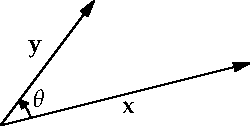
\includegraphics[alt={Vectors and the angle between them in R two}]{dot-angle}
\end{minipage}\smallbreak
As these formulae make clear, the dot product allows us to compute \emph{lengths} of and \emph{angles} between vectors in $\R^2$. An \emph{inner product} is an algebraic structure that generalizes this idea.


\begin{defn}{}{innerproduct}
	Suppose $V$ is a vector space over $\F$ ($=\R$ or $\C$). An \emph{inner product} on $V$ is a function $\ip{\ ,\ }:V\times V\to\F$ satisfying the following properties $\forall\vx,\vy,\vz\in V,\ \lambda\in\F$,
	\begin{enumeratea}\itemsep2pt
	  \item \emph{Linear\footnotemark{} in the first slot}:\quad $\ip{\lambda\vx+\vy,\vz}=\lambda\ip{\vx,\vz}+\ip{\vy,\vz}$
	  \item \emph{Conjugate-Symmetric}:\quad $\ip{\vy,\vx}=\cl{\ip{\vx,\vy}}$ \hfill (complex conjugate!)
	  \item \emph{Positive-definite}:\quad $\vx\neq \V0\implies \ip{\vx,\vx}>0$
	\end{enumeratea}
	We call $\big(V,\ip{\ ,\ }\big)$ an \emph{inner product space}.\smallbreak
	The \emph{norm} or \emph{length} of $\vx\in V$ is $\Nm{\vx}:=\sqrt{\ip{\vx,\vx}}$. A \emph{unit vector} has $\Nm\vx=1$.\smallbreak
	Vectors $\vx,\vy$ are \emph{perpendicular/orthogonal} if $\ip{\vx,\vy}=0$ and \emph{orthonormal} if they are additionally unit vectors.
\end{defn}

\footnotetext{%
	\textcolor{red}{\textbf{Warning!}} In Physics, standard convention is to be \emph{conjugate-linear} in the first slot: $\ip{\lambda\vx+\vy,\vz}=\textcolor{red}{\cl\lambda}\ip{\vx,\vz}+\ip{\vy,\vz}$. If $\F=\R$ this makes no difference. The common Physics notation relates to ours via $\ip{\vx\,|\,\vy}=\ip{\vy,\vx}$.%
}



\boldsubsubsection{Real inner product spaces}\phantomsection\label{sec:realbilinearity}

The definition simplifies slightly when $\F=\R$.
\begin{itemize}
  \item Conjugate-symmetry becomes plain \emph{symmetry}: $\ip{\vy,\vx}=\ip{\vx,\vy}$.
  \item Linearity plus symmetry yields \emph{bilinearity}: a real inner product is also linear in its second slot
  \[
  	\ip{\vx,\lambda\vy+\vz}=\lambda\ip{\vx,\vy}+\ip{\vx,\vz}
  \]
\end{itemize}
A real inner product is often described as a \emph{positive-definite, symmetric, bilinear form.}

\begin{defn}{}{}
	\emph{$n$-dimensional Euclidean space} is $\R^n$ equipped with the \emph{standard inner (dot) product},
	\[
		\ip{\vx,\vy} :=\vx\cdot\vy =\vy^T\vx
		=\sum_{j=1}^nx_jy_j
		=x_1y_1+\cdots+x_ny_n,\qquad 
		\Nm{\vx}=\sqrt{\sum_{j=1}^nx_j^2}
	\]
	Co-ordinates $x_j,y_j$ are with respect to the standard basis $\epsilon=\{\vect en\}$. We call $\Nm{\vx}$ the \emph{Euclidean norm.}
\end{defn}

Unless the inner product is stated explicitly, if we refer to $\R^n$ as an inner product space, we mean Euclidean space. There are, however, many other ways to equip $\R^n$ with an inner product\ldots


\pagebreak[3]


\begin{example}{}{ipsweight}
	Define a new function on $\R^2$ via
	\[
		\ip{\vx,\vy}:=x_1y_1+3x_2y_2
	\]
	It is easy to check that this satisfies the definition of an inner product: 
	\begin{enumeratea}
  	\item \emph{Linearity} follows from the associative/distributive laws in $\R$,
  	\begin{align*}
  		\ip{\lambda\vx+\vy,\vz}
  		&=(\lambda x_1+y_1)z_1+3(\lambda x_2+y_2)z_2
  			=\lambda(x_1z_1+3x_2z_2)+(y_1z_1+3y_2z_2)\\
  		&=\lambda\ip{\vx,\vz}+\ip{\vy,\vz}
  	\end{align*}
  	\item \emph{Symmetry} follows from the commutativity of multiplication in $\R$,
  	\[
  		\ip{\vy,\vx} =y_1x_1+3y_2x_2 =x_1y_1+3x_2y_2 =\ip{\vx,\vy}
  	\]
		\item \emph{Positive-definiteness}: if $\vx\neq\V0$, then $\ip{\vx,\vx}=x_1^2+3x_2^2>0$.
	\end{enumeratea}
	So far, so good. What differs between $\ip{\ ,\ }$ and the standard ``dot'' product is the notion of \emph{orthogonality}. Consider, for instance, $\vx=\frac 12\stwovec 11$ and $\vy=\frac 1{2\sqrt{3}}\stwovec 3{-1}$. With respect to $\ip{\ ,\ }$, $\{\vx,\vy\}$ are \emph{orthonormal}:
  \[
  	\Nm\vx^2=\frac 14(1^2+3\cdot 1^2)=1\qquad 
  	\Nm\vy^2=\frac 1{12}(3^2+3\cdot 1^2)=1\qquad 
  	\ip{\vx,\vy}=\frac 1{4\sqrt 3}(3-3)=0
  \]
  	By contrast, there is nothing special about these vectors with respect to the standard dot product:
  \[
  	\vx\cdot\vx=\frac 12\qquad 
  	\vy\cdot\vy=\frac 56\qquad 
  	\vx\cdot \vy=\frac 1{2\sqrt 3}
  \]
  We have the same \emph{vector space} $\R^2$, but different \emph{inner product spaces}: $(\R^2,\ip{\ ,\ })\neq (\R^2,\cdot)$.
\end{example}

The example is what we call a \emph{weighted inner product}: if we choose \emph{weights} $a_1,\ldots,a_n\in\R^+$, then
\[
	\ip{\vx,\vy} :=\sum_{j=1}^na_jx_jy_j =a_1x_1y_1+\cdots+a_nx_ny_n
\]
defines an inner product on $\R^n$. In this fashion, $\R^n$ may be equipped with \emph{infinitely many distinct inner products}. Even this idea generalizes:
	
\begin{defn}{}{posdefmatrix}
	A symmetric matrix $A\in M_n(\R)$ is \emph{positive-definite} if $\vx^TA\vx>0$ for all non-zero $\vx\in\R^n$.
\end{defn}

If $A$ is positive-definite, it is straightforward to check that $\ip{\vx,\vy}:=\vy^TA\vx$ is an inner product on $\R^n$. In fact (Exercise \ref{exs:allipfn}) \emph{all} inner products on $\R^n$ arise in this fashion! The weighted inner products are when $A$ is diagonal; Euclidean space has $A=I$.
	
\begin{example}{}{ipsweight3}
	The matrix $A=
	\begin{smatrix}
		3&1\\1&1
	\end{smatrix}$
	is positive-definite %($\vx^TA\vx=3x_1^2+2x_1x_2+x_2^2=2x_1^2+(x_1+x_2)^2$) 
	and thus defines an inner product
	\[
		\ip{\vx,\vy} =3x_1y_1+x_1y_2+x_2y_1+x_2y_2
	\]
\end{example}


\pagebreak[3]


\begin{lemm}{Basic properties}{ipbasic}
	Let $V$ be an inner product space, $\vx,\vy,\vz\in V$ and $\lambda\in\F$.
	\begin{enumerate}%\itemsep2pt
		\item \makebox[200pt][l]{$\ip{\V0,\vx}=0$\hfill 2. } $\Nm\vx=0\iff \vx=\V0$
		\setcounter{enumi}{2}
		\item \makebox[200pt][l]{$\Nm{\lambda\vx}=\nm{\lambda}\Nm{\vx}$\hfill 4. } $\ip{\vx,\vz}=\ip{\vy,\vz}$ for all $\vz\Longrightarrow \vx=\vy$
		\setcounter{enumi}{4}
		  \item (Cauchy--Schwarz inequality)\quad $\nm{\ip{\vx,\vy}}\le\Nm\vx\Nm\vy$. Moreover, this is an \textbf{equality} if and only if $\vx,\vy$ are parallel (linearly dependent).
	\end{enumerate}
	\begin{minipage}[t]{0.73\linewidth}\vspace{-8pt}
		\begin{enumerate}[resume]
		  \item (Triangle inequality)\quad $\Nm{\vx+\vy}\le\Nm\vx+\Nm\vy$. This is an \textbf{equality} if and only if $\vx,\vy$ are parallel \textbf{and} point in the same direction.\par
		  As pictured, in $\R^2$ or $\R^3$ this simply says that any side of a triangle is no longer that the sum of the lengths of the other sides.
		\end{enumerate}
  \end{minipage}
  \hfill
	\begin{minipage}[t]{0.24\linewidth}\vspace{-8pt}
  	\hfill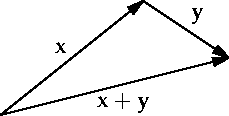
\includegraphics[alt={The triangle inequality}]{dot-triangle}
	\end{minipage}
\end{lemm}


Be careful with notation: $\nm\lambda$ is the \emph{absolute value}/\emph{modulus} of a \emph{scalar}, whereas $\Nm{\vx}$ is the \emph{norm} of a \emph{vector}.\medbreak


	In the real case, we may define the \emph{angle} between non-zero vectors via $\cos\theta=\frac{\ip{\vx,\vy}}{\Nm\vx\Nm\vy}$  ($\in[-1,1]$ by Cauchy--Schwarz!). Outwith Euclidean $\R^2$ and $\R^3$, this notion is of limited application; elsewhere, \emph{orthogonality} and \emph{orthonormality} are typically all we need.


\begin{proof}
	Parts 1--3 are exercises. For simplicity, we prove 5 and 6 only when $\F=\R$.
	\begin{enumerate}\setcounter{enumi}{3}
	%   \item $\ip{\V0,\vx}=\ip{\vx-\vx,\vx}=\ip{\vx,\vx}-\ip{\vx,\vx}=0$
	%   \item ($\Rightarrow$) is the contrapositive of defining property (c), while $(\Leftarrow)$ follows from part 1.
	%   \item $\Nm{\lambda\vx}^2=\ip{\lambda\vx,\lambda\vx}=\lambda\cl\lambda\ip{\vx,\vx}=\nm{\lambda}^2\Nm{\vx}^2$
	  \item Let $\vz=\vx-\vy$, apply the linearity condition and part 2:
	  \[
	  	\ip{\vx,\vz}=\ip{\vy,\vz}
	  	\implies 0=\ip{\vx-\vy,\vz}=\ip{\vx-\vy,\vx-\vy}=\Nm{\vx-\vy}^2
	  	\implies \vx=\vy
	  \]
	  
	  \item If $\vy=\V0$, the result is trivial ($0\vx+\vy=\V0$ is a linear dependence!). Otherwise,
	  \begin{align*}
		  0&\le\Nm{\Nm{\vy}\vx-\frac{\ip{\vx,\vy}}{\Nm{\vy}}\vy}^2 =\ip{\Nm{\vy}\vx-\frac{\ip{\vx,\vy}}{\Nm{\vy}}\vy,\Nm{\vy}\vx-\frac{\ip{\vx,\vy}}{\Nm{\vy}}\vy}\tag{positive-definiteness}\\
		  &=\Nm{\vy}^2\Nm\vx^2 -\ip{\vx,\vy}\ip{\vx,\vy} -\ip{\vx,\vy}\ip{\vy,\vx}  +\nm{\ip{\vx,\vy}}^2 \tag{bilinearity}\\
		  &=\Nm\vx^2\Nm{\vy}^2-\nm{\ip{\vx,\vy}}^2\tag{symmetry}
	  \end{align*}
	  Taking square-roots establishes the inequality. By part 2, equality forces $\Nm{\vy}^2\vx=\ip{\vx,\vy}\vy$: a linear dependence. Conversely, linear dependence (when $\vy\neq \V0$) means $\vx=\lambda\vy$ for some scalar $\lambda$: by part 3, the inequality becomes $\nm\lambda\Nm{\vy}^2=\nm\lambda\Nm{\vy}^2$.
	  
	  \item We establish the square of the required result.
	  \begin{align*}
		  \bigl(\Nm\vx+\Nm\vy\bigr)^2-\Nm{\vx+\vy}^2&=\Nm\vx^2+2\Nm\vx\Nm\vy+\Nm\vy^2-\Nm\vx^2-\ip{\vx,\vy}-\ip{\vy,\vx}-\Nm\vy^2\\
		  &=2\bigl(\Nm\vx\Nm\vy-\ip{\vx,\vy}\bigr)\\
		  &\ge 2\bigl(\Nm\vx\Nm\vy-\nm{\ip{\vx,\vy}}\bigr)\\
		  &\ge 0 \tag{Cauchy--Schwarz}
	  \end{align*}
	  Equality requires both equality in Cauchy--Schwarz ($\vx,\vy$ parallel) and that $\ip{\vx,\vy}\ge 0$; since $\vx,\vy$ are already parallel, this means that one is a non-negative multiple of the other.\qedhere
	\end{enumerate}
\end{proof}


\pagebreak[3]


\boldsubsubsection{Complex Inner Product Spaces}

Definition \ref{defn:innerproduct} works perfectly when $\C=\F$. The subtle difference comes from how we expand linear combinations in the \emph{second slot}. The proof is easy if you remember your complex conjugates; try it!

\begin{lemm}{}{}
	A complex inner product is a \emph{positive-definite, conjugate-symmetric, \textcolor{red}{sesquilinear}\footnotemark{} form}: it is \emph{conjugate-linear} in the second slot,
	\[
		\ip{\vx,\lambda\vy+\vz}=\textcolor{red}{\cl\lambda}\ip{\vx,\vy}+\ip{\vx,\vz}
	\]
\end{lemm}

\footnotetext{%
	The prefix \emph{sesqui-} means \emph{one-and-a-half}; for instance a \emph{sesquicentenary} is a 150 year anniversary.%
} 

When $\F=\R$ this is \emph{bilinearity} (page \pageref{sec:realbilinearity}): $\ip{\vx,\lambda\vy+\vz}=\lambda\ip{\vx,\vy}+\ip{\vx,\vz}$. Since it costs nothing to write abstract inner product spaces as if they are complex, almost all results will cover the real and complex cases simultaneously, though occasionally a different proof will be required. If you don't feel confident with complex numbers, at first read let $\F=\R$ and delete all complex conjugates! %For simplicity, most examples will use real inner products. 


\begin{defn}{}{}
	The \emph{standard (Hermitian) inner product} and \emph{norm} on $\C^n$ are
	\[
		\ip{\vx,\vy} :=\vy^*\vx 
		=\sum_{j=1}^nx_j\cl{y_j}
		=x_1\cl{y_1}+\cdots+x_n\cl{y_n},\qquad 
		\Nm{\vx}=\sqrt{\sum_{j=1}^n\nm{x_j}^2}
	\]
	where $\vy^*=\cl\vy^T$ is the \emph{conjugate-transpose\footnotemark{}} of $\vy$ and $\nm{x_j}=\sqrt{x_j\cl{x_j}}$ is the \emph{modulus.}
\end{defn}

\footnotetext{%
	The physics convention (conjugate-linearity in the \textbf{first} slot) is arguably superior for Hermitian inner products, since $\ip{\vx\,|\,\vy}=\vx^*\vy =\cl{\vx}^T\vy$ keeps $\vx,\vy$ in the same order, whereas our notation ($\ip{\vx,\vy}=\vy^*\vx$) reverses them.%
}

\begin{example}{}{}
	The vectors $\vx=\stwovec{1+i}{i}$ and $\vy=\stwovec{i}{1-i}$ are (Hermitian-)orthogonal:
	\[
		\ip{\vx,\vy}=\vy^*\vx =\big(-i\quad 1+i\big)\twovec{1+i}{i} =-i(1+i)+(1+i)i =0
	\]
\end{example}

Weighted inner products may be defined as on page \pageref{ex:ipsweight} (the weights $a_j$ must still be \emph{positive real numbers}):
\[
	\ip{\vx,\vy} :=\sum_{j=1}^na_jx_j\cl{y_j}
	=a_1x_1\cl{y_1}+\cdots+a_nx_n\cl{y_n}
\]
We may similarly define inner products in terms of positive-definite matrices $\ip{\vx,\vy}:=\vy^*A\vx$.

\begin{defn}{}{}
	A matrix $A\in M_n(\C)$ is \emph{self-adjoint (Hermitian)} if $A^*=A$. A self-adjoint matrix is \emph{positive-definite} if $\vx^*A\vx>0$ for all non-zero $\vx\in\C^n$.
\end{defn}

Self-adjoint means symmetric ($A^T=A$) if $A$ is a real matrix.

\begin{example}{}{}
	Exercise \ref{exs:complexposdef} verifies that $A=
	\begin{smatrix}
		3&-i\\i&3
	\end{smatrix}$ is positive-definite. We therefore obtain an new inner product on $\C^2$:
	\[
		\ip{\vx,\vy}=\bigl(\cl{y_1}\ \ \cl{y_2}\bigr)
		\begin{pmatrix}
			3&-i\\i&3
		\end{pmatrix}
		\twovec{x_1}{x_2} =
		3x_1\cl{y_1}+ix_1\cl{y_2}-ix_2\cl{y_1}+3x_2\cl{y_2}
	\]
\end{example}


\pagebreak[3]


\boldsubsubsection{Further Examples of Inner Product Spaces}

As always when discussing inner products, the field $\F$ must be either $\R$ or $\C$.

\begin{defn}{Frobenius inner product}{}
	If $A,B\in M_{m\times n}(\F)$, define
	\[
		\ip{A,B}=\tr(B^*A) =\sum_{j=1}^m\sum_{k=1}^n \cl{b_{kj}}a_{jk}
	\]
	where $\tr$ is the \emph{trace} of an $n\times n$ matrix. This makes $M_{m\times n}(\F)$ into an inner product space.
\end{defn}

This isn't really a new example: if we map $M_{m\times n}(\F)\to\F^{m\times n}$ by stacking the columns of our matrices, then the Frobenius inner product is the standard (Hermitian/dot) inner product in disguise.


\begin{example}{}{frobenius}
	In $M_{3\times 2}(\C)$,
	\begin{gather*}
		\begin{aligned}
			\ip{
				\begin{pmatrix}
					1&i\\
					2-i&0\\
					0&-1
				\end{pmatrix}
				,
				\begin{pmatrix}
					0&7\\
					1&2i\\
					3-2i&4
				\end{pmatrix}
			}
			&=\tr
			\begin{pmatrix}
				0&1&3+2i\\
				7&-2i&4
			\end{pmatrix}
			\begin{pmatrix}
				1&i\\
				2-i&0\\
				0&-1
			\end{pmatrix}
			=\tr
			\begin{pmatrix}
				2-i&-3-2i\\
				9-4i&-4+7i
			\end{pmatrix}\\
			&=(2-i)+(-4+7i) =-2-8i
		\end{aligned}\\
		\begin{aligned}
			\Nm{
				\begin{pmatrix}
					1&i\\
					2-i&0\\
					0&-1
				\end{pmatrix}
			}^2
			&=\tr
			\begin{pmatrix}
				1&2+i&0\\
				-i&0&-1
			\end{pmatrix}
			\begin{pmatrix}
				1&i\\
				2-i&0\\
				0&-1
			\end{pmatrix}
			=\tr
			\begin{pmatrix}
				6&i\\
				-i&2
			\end{pmatrix}
			=8
		\end{aligned}
	\end{gather*}
\end{example}


\begin{defn}{$L^2$ inner product}{}
	Given a \emph{real} interval $[a,b]$, the function
	\[
		\ip{f,g}:=\int_a^b f(t)\cl{g(t)}\,\dt
	\]
	defines an inner product on the space $C[a,b]$ of continuous functions $f:[a,b]\to\F$.
\end{defn}


Verifying Definition \ref{defn:innerproduct} is straightforward with a little analysis; for instance continuity allows us to conclude
\[
	\Nm f^2=\int_a^b\nm{f(x)}^2\,\dx=0\iff f(x)\equiv 0
\]
This is our first example of an \emph{infinite-dimensional} inner product space. With careful restriction, this works even for infinite intervals and a larger class of functions.\footnote{%
	For us, functions will always be continuous (often polynomials) on closed bounded intervals. The \emph{square-integrable functions} and \emph{$L^2$-spaces} for which the inner product is named are a more complicated business and beyond this course.%
}

\begin{example}{}{}
	Let $f(x)=x$ and $g(x)=x^2$. These lie in the $L^2$ inner product space $C[-1,1]$. Indeed,
	\[
		\ip{f,g}=\int_{-1}^1x^3\,\dx=0\qquad 
		\Nm f^2=\int_{-1}^1x^2\,\dx=\frac 23\qquad 
		\Nm g^2=\int_{-1}^1x^4\,\dx=\frac 25
	\]
	With some simple scaling, we see that $\frac 1{\Nm f}f=\sqrt{\frac 32}x$ and $\frac 1{\Nm g}g=\sqrt{\frac 52}x^2$ are orthonormal.
\end{example}


\pagebreak[3]


\begin{defn}{$\ell^2$ inner product}{ell2ip}
	A sequence $(x_n)$ of real or complex numbers is \emph{square-summable} if the series $\sum\nm{x_n}^2$ converges. It can be shown that the set of such sequences forms a vector space on which we can define an inner product\footnotemark{}
	\[
		\ip{(x_n),(y_n)}=\sum_{n=1}^\infty x_n\cl{y_n}
	\]
\end{defn}

\footnotetext{%
	Neither of these facts are obvious; for instance, we'd need to see that the sum of two square-summable sequences is also square-summable, and that being square-summable forces the inner product series to converge\ldots%
}

In essence, this is the standard inner product on $\F^n$ after letting $n\to\infty$! This example, and its $L^2$ cousin, are the prototypical \emph{Hilbert spaces,} which have great application to differential equations, signal processing, etc. While we will certainly compute with these examples, a rigorous discussion requires significant input from analysis (convergence of series, completeness, integrability), which would take us too far afield.



\begin{exercises}
	\exstart Evaluate the inner product of each pair of vectors.
	\begin{enumerate}\setcounter{enumi}{1}
	  \item[]\begin{enumerate}
	    \item $\vx=\sthreevec 121$, $\vy=\sthreevec{1}{-1}1$ where $\ip{\vx,\vy}=2x_1y_1+3x_2y_2+x_3y_3$.
	    
	    \item $\vx=\stwovec 1{2i}$, $\vy=\stwovec{5i}{4}$ where $\ip{\vx,\vy}$ is the standard Hermitian inner product on $\C^2$.
	    
	    \item $\vx=\stwovec 1{2i}$, $\vy=\stwovec{5i}{4}$ where $\ip{\vx,\vy}=\vy^*
	    \begin{smatrix}
	    	2&-i\\i&2
	    \end{smatrix}
	    \vx$.
	    
	    \item $f(x)=x-1$, $g(x)=x+1$ where $\ip{f,g}$ is the $L^2$ inner product on $C[0,2]$.
	  \end{enumerate}
	  
	  
	  \item Suppose $\ip{\vx,\vy}=\ip{\vx,\vz}$ for all $\vx$. Prove that $\vy=\vz$.
	  
	  
	  \item Suppose $\vz$ is a constant vector in an inner product space $V$. The linearity condition says that the map $\rT_\vz:V\to\F$ defined by
	  \[
	  	\rT_\vz(\vx):=\ip{\vx,\vz}
	  \]
	  is linear. What, if anything, can you say about the function $\rU_\vz:\vx\mapsto\ip{\vz,\vx}$?
	  
	  
	  \item Define $\ip{\vx,\vy}:=\sum\limits_{j=1}^nx_jy_j$ on $\C^n$. Is this an inner product? Which of the properties (a), (b), (c) from Definition \ref{defn:innerproduct} does it satisfy?
	  
	  
	  \item\begin{enumerate}
	    \item Verify that the matrix in Example \ref{ex:ipsweight3} is positive-definite, so that
	    \[
	    	\ip{\vx,\vy}=3x_1y_1+x_1y_2+x_2y_1+x_2y_2
	    \]
	    really does define an inner product on $\R^2$.\par
	  	(\emph{Hint: Try to write $\Nm{\vx}^2$ as a sum of squares})
	  	
	  	\item Let $\vx=\stwovec 11$. With respect to the inner product in part (a), find a non-zero unit vector $\vy$ which is \emph{orthogonal} to $\vx$.
	  \end{enumerate}

	  
	  \item\label{exs:complexposdef} By multiplying out $\nm{x_1-ix_2}^2$, show that the matrix $\begin{smatrix}3&-i\\i&3\end{smatrix}$ is positive-definite.\smallbreak
	  (\emph{Hint: recall that $\nm{a}^2=a\cl a$ for complex numbers!!!})

	  
	  \item Show that every eigenvalue of a positive definite matrix is positive.
	  
	  
	  \item Prove parts 1, 2 and 3 of Lemma \ref{lemm:ipbasic}.
	  
	  
	  \item\label{exs:pythag} (Pythagorean Theorem) \ Let $V$ be an inner product space. If $\vx,\vy$ are orthogonal, prove
	  \[
	  	\Nm{\vx+\vy}^2=\Nm{\vx}^2+\Nm{\vy}^2
	  \]
	  
	  
		\item Use elementary algebra to prove the Cauchy--Schwarz inequality for vectors $\vx=\stwovec ab$ and $\vy=\stwovec cd$ in $\R^2$ with the standard (dot) product.
		
		
		\item Prove the Cauchy--Schwarz and triangle inequalities for a \emph{complex} inner product space. What has to change compared to the proof of Lemma \ref{lemm:ipbasic}?
		
		
		\item The \emph{polarization identities} demonstrate that if you know the length of every vector, then you know the inner product! Verify them both:
		\begin{enumerate}
		  \item In any real inner product space, $\ip{\vx,\vy}=\frac 14\Nm{\vx+\vy}^2 -\frac 14\Nm{\vx-\vy}^2$
		  \item In any complex inner product space, $\ip{\vx,\vy}=\frac 14\sum\limits_{k=1}^4i^k\Nm{\vx+i^k\vy}^2$
		\end{enumerate}
		
		
		\item Use the Cauchy--Schwarz inequality on a suitable inner product space to prove that
		\[
			\int_0^2\frac{\sqrt x}{x+1}\,\dx\le \frac 2{\sqrt 3}
		\]
	
	  
	  \item\label{exs:fourier} (Fourier Series basis) \ Let $m\in\Z$ and consider the complex-valued function $f_m(x)=\frac 1{\sqrt{2\pi}}e^{i mx}$. Prove that the functions $f_m$ are pairwise orthonormal 
	  \[
	  	\ip{f_m,f_n}=
	  	\begin{cases}
	  		1&\text{if $m=n$}\\
	  		0&\text{if $m\neq n$}
	  	\end{cases}
	  \]
	  with respect to the $L^2$ inner product on $C[-\pi,\pi]$.\par
	  (\emph{Hint: If complex functions are scary, use Euler's formula $e^{i mx}=\cos mx+i\sin mx$ and work with the real-valued functions $\cos mx$ and $\sin mx$. The difficulty is that you then need integration by parts\ldots})
	  
	  
	  \item\label{exs:allipfn} Let $\ip{\ ,\ }$ be an inner product on $\F^n$. Define the matrix $A\in M_n(\F)$ by $A_{jk}=\ip{\ve_k,\ve_j}$ where $\{\vect en\}$ is the standard basis. Verify that $A$ is the \emph{matrix of the inner product}:
	  \[
	  	\forall \vx,\vy\in\F^n,\ \ip{\vx,\vy}=\vy^*A\vx
	  \]
	  In particular, $A$ is \emph{self-adjoint} ($A^*=A$) and \emph{positive-definite} ($\vx\neq\V0\Longrightarrow \vx^*A\vx>\V0$).\par
	  \emph{More generally, if $\beta=\{\vect vn\}$ is a basis of any finite-dimensional inner product space, then $A_{jk}=\ip{\vv_k,\vv_j}$ defines the matrix of the inner product with respect to $\beta$:}
	  \[
	  	\ip{\vx,\vy}=[\vy]_\beta^*A[\vx]_\beta
	  \]
	\end{enumerate}
\end{exercises}


\clearpage




\subsection{Orthogonal Subspaces and the Gram--Schmidt Process}\label{sec:gs}


In finite dimensions, linear algebra can sometimes feel purely algorithmic: evaluate the co-ordinates of every vector with respect to a basis $\beta=\{\vect vn\}$,
\[
	\vx=\sum_{k=1}^na_k\vv_k=\lincom a{v}n 
	\quad\longrightsquigarrow\quad  
	[\vx]_\beta=\threevec{a_1}{\vdots}{a_n} \tag{$\ast$}
\]
and use matrix multiplication to represent linear maps. In practice, finding the co-ordinates can be tedious (many row operations). If, however, $\beta$ is an \emph{orthogonal} basis, then this becomes almost trivial.


\begin{lemm}{}{orthcalc}
	Let $V$ be an inner product space and $\beta=\{\vect{\vv}{n}\}$ an orthogonal spanning set of non-zero vectors:
	\[
		V=\Span\beta
		\quad\text{and}\quad
		\ip{\vv_j,\vv_k}=
		\begin{cases}
			0&\text{if $j\neq k$}\\
			\Nm{\vv_j}^2\neq 0&\text{if $j=k$}
		\end{cases}
	\]
	Then $\beta$ is a basis of $V$ and each $\vx\in V$ has unique representation
  \[
  	\vx=\sum\limits_{k=1}^n\frac{\ip{\vx,\vv_k}}{\Nm{\vv_k}^2}\vv_k
  	\tag*{$\left(a_k=\frac{\ip{\vx,\vv_k}}{\Nm{\vv_k}^2}\text{ in }(\ast)\right)$}
  \]
  This simplifies to $\vx=\sum\ip{\vx,\vv_k}\vv_k$ if $\beta$ is an orthonormal set.
\end{lemm}

\begin{proof}
  Since $\beta$ spans $V$, any given $\vx\in V$ may be written as a linear combination $(\ast)$. Simply take the inner product with each basis vector in turn, and apply the orthogonality of $\beta$:
  \[
		\ip{\vx,\vv_j}=\sum_{k=1}^na_k\ip{\vv_k,\vv_j}=a_j\Nm{\vv_j}^2
	\]
 	Finally, let $\vx=\V0$ to see that $\beta$ is linearly independent ($\lincom a{v}n=\V0\Longrightarrow a_k=0$).
\end{proof}


\begin{examples}{}{}
	\exstart Let $\vx=\stwovec{x_1}{x_2} =x_1\ve_1+x_2\ve_2$ with respect to the standard orthonormal basis $\beta=\{\ve_1,\ve_2\}$ of $\R^2$. We easily check that
  \[
  	\sum_{k=1}^2\ip{\vx,\ve_k}\ve_k =x_1\ve_1+x_2\ve_2 =\vx
  \]
  \begin{enumerate}\setcounter{enumi}{1}
    \item In Euclidean $\R^3$, $\beta=\{\vv_1,\vv_2,\vv_3\}=\left\{\sthreevec 123,\sthreevec 2{-1}0,\sthreevec 36{-5}\right\}$ is an orthogonal set and thus a basis. We compute the co-ordinates of $\vx=\sthreevec 742$ with respect to $\beta$:\vspace{-3pt}
	\begin{align*}
		\vx
		&=\sum_{k=1}^3\frac{\ip{\vx,\vv_k}}{\Nm{\vv_k}^2}\vv_k 
			=\frac{7+8+6}{1+4+9}\threevec 123 
			+\frac{14-4+0}{4+1+0}\threevec 2{-1}0 
			+\frac{21+24-10}{9+36+25}\threevec 36{-5}\\
		&=\frac 32\threevec 123 + 2\threevec 2{-1}0 + \frac 12\threevec 36{-5} 
			\implies [\vx]_\beta=\threevec{3/2}{2}{1/2}
	\end{align*}
	Compare this with the painfully slow augmented matrix method for finding co-ordinates!
	
	\pagebreak[3]
	
    \item With respect to the standard inner product on $\C^2$, $\beta=\{\vv_1,\vv_2\} =\bigl\{\stwovec 1{i},\stwovec i1\bigr\}$ forms an orthogonal basis (each vector has norm $\sqrt 2$). Given $\vx=\stwovec{1+i}{3i}$, observe that
	  \begin{align*}
	  	\sum_{k=1}^2\frac{\ip{\vx,\vv_k}}{\Nm{\vv_k}^2}\vv_k
	  	&=\frac{\ip{\stwovec{1+i}{3i},\stwovec{1}{i}}}{2}\twovec{1}{i} 
	  	+
	  	\frac{\ip{\stwovec{1+i}{3i},\stwovec{i}{1}}}{2}\twovec{i}{1}\\
	  	&=\frac{(1+i)(1)+(3i)(-i)}{2}\twovec{1}{i} 
	  	+
	  	\frac{(1+i)(-i)+(3i)(1)}{2}\twovec{i}{1}\\
	  	&=\frac{4+i}{2}\twovec{1}{i}
	  	+\frac{1+2i}2\twovec{i}{1} =\vx	 
	  \end{align*}
	  Otherwise said, $[\vx]_\beta=\frac 12\stwovec{4+i}{1+2i}$.
  \end{enumerate}
\end{examples}


\boldsubsubsection{Orthogonal Subspaces, Complements and Projections}

Given the practical benefit of an orthogonal/orthonormal basis, the obvious question is ``How do we find one?'' For this purpose, and for other reasons, it is helpful to discuss how subspaces interact with the structure of an inner product. 

\begin{defn}{}{orthcomp}
	Let $V$ be an inner product space and $U$ a subspace. The \emph{orthogonal complement} $U^\perp$ is
	\[
		U^\perp =\big\{\vx\in V:\forall\vu\in U,\ \ip{\vx,\vu}=0\big\}
	\]
	More generally, subspaces $U,W$ are \emph{orthogonal} if
	\[
		\forall \vu\in U,\ \vw\in W,\ \ip{\vu,\vw}=0
	\]
\end{defn}


\begin{example}{}{orthcompeeasy}
	Given the subspace $U=\Span\left\{\sthreevec 100,\sthreevec 0{-1}3\right\}$ of Euclidean $\R^3$, we see that
	\[
		U^\perp
		=\left\{ \vx\in\R^3:\vx\cdot\sthreevec 100=0=\vx\cdot\sthreevec 0{-1}3\right\}
		=\Span\sthreevec 031
	\]
\end{example}

The example certainly suggests that $U^\perp$ is a subspace. This, and much else, holds in general.

\begin{lemm}{}{uperpperp}
	Suppose $U$ is a subspace of an inner product space $V$. Then:
	\begin{enumeratea}
    \item $U^\perp$ is a subspace of $V$.
    \item $U\cap U^\perp=\{\V0\}$.
    \item $U\le (U^\perp)^\perp$. In particular, $U$ and $U^\perp$ are orthogonal subspaces (Definition \ref{defn:orthcomp}).
    \item If $V=U\oplus U^\perp$, then $U=(U^\perp)^\perp$.
	\end{enumeratea}
\end{lemm}

We leave the proof to Exercise \ref{exs:uperpperp}. Theorem \ref{thm:orthcalc} and Corollary \ref{cor:orthbasis} will show that $V=U\oplus U^\perp$ (and thus $(U^\perp)^\perp=U$) always holds when $\dim U$ is finite. It is perhaps surprising that (c) need not be equality in infinite dimensions (Exercise \ref{ex:ell2ex}).


\boldinline{Orthogonal Projections}

As in the example and part (d) of the Lemma, it is common to have a direct sum decomposition $V=U\oplus U^\perp$. Recall what this means:
\[
	\forall \vx\in V, \exists \text{ \emph{unique} }\vu\in U,\vw\in U^\perp \text{ such that }\vx=\vu+\vw
\]

\begin{minipage}[t]{0.64\linewidth}\vspace{-5pt}
	In such a situation, the vectors $\vu=\pi_U(\vx)$, $\vw=\pi^\perp_U(\vx)$ are called the \emph{orthogonal projections} of $\vx$ onto the subspaces $U,U^\perp$. Indeed the orthogonal projections can be thought of as \emph{functions}
	\[
		\pi_U:V\to U,\quad \pi_{U^\perp}:V\to\ U^\perp
	\]
\end{minipage}
\hfill
\begin{minipage}[t]{0.35\linewidth}\vspace{-45pt}
	\hfill
	\href{https://www.math.uci.edu/~ndonalds/math121b/gram-orthproj.html}{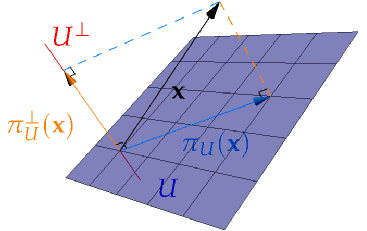
\includegraphics[scale=0.9]{gram-orthproj}}
\end{minipage}\smallbreak
Orthogonal projections are crucial both theoretically and in applications. We'll discuss them repeatedly in future sections.\par
As our next result shows, orthogonal projections are simple when $U$ has a \emph{finite orthogonal basis}.


\begin{thm}{}{orthcalc}
	Let $V$ be an inner product space. Suppose $\beta=\{\vect{\vu}{n}\}$ is a set of orthogonal non-zero vectors and let $U=\Span\beta$. Then $V=U\oplus U^\perp$.\par
	More specifically, every $\vx\in V$ decomposes uniquely in the form $\vx=\vu+\vw$ where
  \[
  	\vu =\pi_U(\vx)=\sum\limits_{k=1}^n\frac{\ip{\vx,\vu_k}}{\Nm{\vu_k}^2}\vu_k\in U
  	\quad\text{and}\quad 
  	\vw=\pi^\perp_U(\vx)=\vx-\vu\in U^\perp
  \]
\end{thm}

\begin{proof}
	Since $U$ is an inner product space in its own right, Lemma \ref{lemm:orthcalc} says that $\beta$ is a basis of $U$.\smallbreak
	Now consider $\vu,\vw$ as defined. Plainly $\vu\in \Span\beta=U$. For each $\vu_j$, the orthogonality of $\beta$ tells us that
  \begin{align*}
  	\ip{\vw,\vu_j}
  	&=\ip{\vx-\vu,\vu_j} =\ip{\vx,\vu_j}-\ip{\vu,\vu_j}
  	=\ip{\vx,\vu_j}-\ip{\sum_{k=1}^n\frac{\ip{\vx,\vu_k}}{\Nm{\vu_k}^2}\vu_k,\vu_j}\\
  	&=\ip{\vx,\vu_j}-\sum_{k=1}^n\frac{\ip{\vx,\vu_k}}{\Nm{\vu_k}^2}\ip{\vu_k,\vu_j}\\
  	&=\ip{\vx,\vu_j}-\ip{\vx,\vu_j}=0
  \end{align*}
  Since $\vw$ is orthogonal to a basis of $U$, it follows that $\vw$ is orthogonal to any element of $U$; we conclude that $\vw\in U^\perp$.\par
  Finally, suppose $\vx=\vu_1+\vw_1$ for some $\vu_1\in U$, $\vw_1\in U^\perp$. Then
  \[
  	\vx=\vu_1+\vw_1=\vu+\vw\implies \vu_1-\vu=\vw-\vw_1 \in U\cap U^\perp =\{\V0\}
  \]
  by Lemma \ref{lemm:uperpperp}. We conclude that the decomposition $\vx=\vu+\vw$ is unique, and that $V=U\oplus U^\perp$ is indeed a direct sum.
\end{proof}


\begin{example}{}{}
	Revisiting Example \ref{ex:orthcompeeasy}, we project $\vx=\sthreevec 111$ onto $U=\Span\left\{\sthreevec 100,\sthreevec 0{-1}3\right\}$:
	\[
		\pi_U(\vx)=\frac{1}{1}\threevec 100+\frac{2}{10}\threevec 0{-1}3=\frac 15\threevec 5{-1}3,\qquad \pi_U^\perp(\vx)=\vx-\pi_U(\vx)=\frac 25\threevec 031
	\]
\end{example}


\pagebreak[3]


\boldsubsubsection{The Gram--Schmidt Process}

Theorem \ref{thm:orthcalc} tells us how to compute the orthogonal projections corresponding to $V=U\oplus U^\perp$, \emph{provided $U$ has a finite, orthogonal basis.} Given the usefulness of such a set-up, our next goal is to see how to construct such. Thankfully there exists a straightforward algorithm.

\begin{thm}{Gram--Schmidt}{gs}
	Suppose $S=\{\vect{\vs}{n}\}$ is a \textbf{finite} linearly independent subset of an inner product space $V$. Inductively construct a sequence of vectors $\vect{\vu}{n}$:
	\[
		\vu_k:=\vs_k-\sum_{j=1}^{k-1}\frac{\ip{\vs_k,\vu_j}}{\Nm{\vu_j}^2}\vu_j
		\tag{$\vu_k=\pi^\perp_{U_{k-1}}(\vs_k)$ where $U_{k-1}=\Span\{\vect u{k-1}\}$}
	\]
	Then $\beta:=\{\vect{\vu}{n}\}$ is an orthogonal basis of $\Span S$.
\end{thm}

In examples, we often choose non-zero multiples $\vu_k=a_k\pi^\perp_{U_{k-1}}(\vs_k)$ so as to avoid fractions. If you want an \emph{orthonormal} basis, it is usually easier to scale everything after the algorithm is complete.

\begin{example}{}{gs1}
	$S=\{\vs_1,\vs_2,\vs_3\}=\left\{\sthreevec 100,\sthreevec 2{-1}3,\sthreevec 111\right\}$ is a linearly independent subset of $\R^3$.
	\begin{enumerate}
	  \item Choose $\vu_1=\vs_1=\sthreevec 100$. Observe that $\Nm{\vu_1}^2=1$
	  \item Choose $\vu_2=\vs_2-\frac{\ip{\vs_2,\vu_1}}{\Nm{\vu_1}^2}\vu_1=\sthreevec 2{-1}3-\frac{2}{1}\sthreevec 100 =\sthreevec 0{-1}3$. Observe that $\Nm{\vu_2}^2=10$.
	  \item $\pi_{U_2}^\perp(\vs_3)=\vs_3-\frac{\ip{\vs_3,\vu_1}}{\Nm{\vu_1}^2}\vu_1 -\frac{\ip{\vs_3,\vu_2}}{\Nm{\vu_2}^2}\vu_2=\sthreevec 111-\frac{1}{1}\sthreevec 100 -\frac{2}{10}\sthreevec 0{-1}3 =\frac 25\sthreevec 0{3}{1}$. We choose $\vu_3=\sthreevec 03{1}$.
	\end{enumerate}
	Plainly $\beta=\left\{\sthreevec 100,\sthreevec 0{-1}3,\sthreevec 031\right\}$ is an orthogonal basis of $\R^3$.
\end{example}


\begin{proof}
	For each $k\le n$, define $S_k=\{\vect{\vs}{k}\}$ and $\beta_k=\{\vect{\vu}{k}\}$. We prove by induction that each $\beta_k$ is an orthogonal basis of $U_k:=\Span\beta_k=\Span S_k$. The Theorem is the terminal case $k=n$.
	\begin{description}
		\item[\normalfont (Base case $k=1$)] Certainly $\beta_1=\{a_1\vs_1\}$ is an orthogonal set and $U_1=\Span\beta_1=\Span S_1$.
		\item[\normalfont	(Induction step)] Fix $k\ge 2$ and assume $\beta_{k-1}$ is an orthogonal basis of $U_{k-1}=\Span S_{k-1}$. By Theorem \ref{thm:orthcalc}, $\vu_k=\pi_{U_{k-1}}^\perp(\vs_k)\in U_{k-1}^\perp$. We also see that $\vu_k\neq \V0$, for if not,
		\[
			\vs_k =\sum_{j=1}^{k-1}\frac{\ip{\vs_k,\vu_j}}{\Nm{\vu_j}^2}\vu_j\in U_{k-1}=\Span S_{k-1}
		\]
		and $S$ would be linearly dependent. It follows that $\beta_k$ is an orthogonal set of non-zero vectors, and thus (Theorem \ref{thm:orthcalc}) a basis for $U_k=\Span\beta_k$. Moreover,
		\[
			\vs_k=\vu_k+\sum_{j=1}^{k-1}\frac{\ip{\vs_k,\vu_j}}{\Nm{\vu_j}^2}\vu_j\in U_k \implies \Span S_k\le U_k
		\]
		Since these spaces have the same (finite) dimension $k$, we conclude that $U_k=\Span S_k$.\qedhere
	\end{description}
\end{proof}



\pagebreak[3]


\begin{example}{}{ell201}
	We work in the space of real polynomials $P(\R)$ equipped with the $L^2$ inner product $\ip{f,g}=\int_0^1f(x)g(x)\,\dx$. Let $S=\{1,x,x^2\}$ and apply the algorithm (we write $\beta=\{f_1,f_2,f_3\}$):
	\begin{enumerate}
		\item Choose $f_1(x)=1$. We have $\Nm{f_1}^2=\int_0^11\,\dx=1$.
		\item We project the second polynomial $x$ away from $\Span f_1$:
		\[
			\pi_{\Span f_1}^\perp(x)
			=x-\frac{\ip{x,f_1}}{\Nm{f_1}^2}f_1
			=x-\int_0^1x\,\dx 
			=x-\frac 12
		\]
		For simplicity, choose $f_2(x)=2x-1$ with $\Nm{f_2}^2=\int_0^1\left(2x-1\right)^2\,\dx=\frac 13$.
		\item	Repeat, projecting the third supplied polynomial $x^2$ away from $\Span\{ f_1,f_2\}$:
		\begin{align*}
			\pi_{\Span\{f_1,f_2\}}^\perp(x^2) 
			&=x^2-\frac{\ip{x^2,f_1}}{\Nm{f_1}^2}f_1-\frac{\ip{x^2,f_2}}{\Nm{f_2}^2}\\
			&=x^2-\int_0^1x^2\,\dx-\frac{\int_0^1x^2\left(2x-1\right)\,\dx}{1/3}\left(2x-1\right)\\
			&=x^2-x+\frac 16
		\end{align*}
		We choose $f_3(x)=6x^2-6x+1$ with $\Nm{f_3}^2=\int_0^1\left(6x^2-6x+1\right)^2\,\dx=\frac 1{5}$
	\end{enumerate}
	It follows that $\Span S$ has an orthonormal basis
	\[
		\beta=\left\{1,\sqrt 3(2x-1),\sqrt 5(6x^2-6x+1)\right\}
	\]
	This example can be extended to arbitrary degree since the countable set $\{1,x,x^2,\ldots\}$ is a basis of $P(\R)$. Indeed this shows that $\big(P(\R),\ip{\ ,\ }\big)$ has an orthonormal basis.\bigbreak
	For a taste of how Gram--Schmidt and orthogonal projections may be applied, we use this example to find  a \textcolor{Green}{straight-line approximation} to the \textcolor{blue}{parabola} $x^2$ on the interval $[0,1]$.\par
	\begin{minipage}[t]{0.67\linewidth}\vspace{0pt}
		Let $U=\Span\{1,x\}$. As we've just seen, this has orthonormal basis $\big\{1,\sqrt 3(2x-1)\big\}$. Now compute:
		\begin{align*}
		 	\pi_U(x^2)
		 	&=\ip{x^2,1} +\ip{x^2,\sqrt 3(2x-1)}\sqrt 3(2x-1)\\
		 	&=\int_0^1x^2\,\dx +3\left(\int_0^12x^3-x^2\,\dx\right)(2x-1)\\
		 	&=x-\frac 16
		\end{align*}
	\end{minipage}
	\hfill
 	\begin{minipage}[t]{0.3\linewidth}\vspace{0pt}
 		\hfill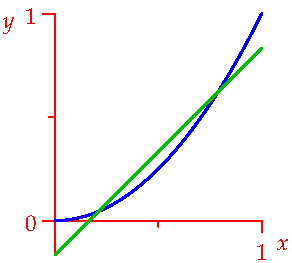
\includegraphics[alt={A linear approximation to y equals x squared on the interval 0 to 1}]{gram-xsquaredapprox}
 	\end{minipage}\smallbreak
	As we'll see later, $u(x)=x-\frac 16$ is the unique linear polynomial which minimizes the function $\Nm{x^2-u(x)}^2=\int_0^1(x^2-u(x))^2\,\dx$. This is a different criteria to what you would be used to in calculus, though $u(x)$ plainly approximates the parabola better than any tangent line would.
\end{example}


\pagebreak[3]


We finish with a book-keeping corollary.

\begin{cor}{}{orthbasis}
	\exstart Every finite-dimensional inner product space has an orthonormal basis.
 	\begin{enumerate}\setcounter{enumi}{1}
 	  \item If $U$ is a finite-dimensional subspace of an inner product space $V$, then $V=U\oplus U^\perp$ and the orthogonal projections may be computed as in Theorem \ref{thm:orthcalc}.
 	\end{enumerate}
\end{cor}

  
\begin{proof}
	\exstart If $V$ is finite-dimensional, take any basis $S=\{\vect sn\}$, apply Gram--Schmidt and normalize the result.
	\begin{enumerate}\setcounter{enumi}{1}
	  \item By part 1, $U$ has an orthonormal basis. Theorem \ref{thm:orthcalc} therefore applies. \qedhere
	\end{enumerate}
\end{proof}

If $U$ is an \emph{infinite-dimensional subspace} of $V$, then we need not have $V=U\oplus U^\perp$ and the orthogonal projections might not be well-defined (see, for example, Exercises \ref{ex:ell2ex} and \ref{ex:fourierx}). Instead, if $\beta$ is an orthonormal basis of $U$, it is common to describe the coefficients $\ip{\vx,\vu}$ for each $\vu\in\beta$ as the \emph{Fourier coefficients}, and the infinite sum
\[
	\sum_{\vu\in\beta}\ip{\vx,\vu}\vu
\]
as the \emph{Fourier series} of $\vx$, provided this sum converges.

  
\bigskip

TIDY EXERCISES!

\begin{exercises}{}{}
\exstart Apply Gram--Schmidt to obtain an orthogonal basis $\beta$ for $\Span S$. Then obtain the co-ordinate representation (Fourier coefficients) of the given vector with respect to $\beta$.
\begin{enumerate}\setcounter{enumi}{1}
  \item[]\begin{enumerate}
    \item $S=\left\{\sthreevec 111,\sthreevec 011,\sthreevec 001\right\}\subseteq\R^3$,\quad $\vx=\sthreevec 101$
    \item $S=\left\{
    \begin{smatrix}
    3&5\\-1&1
    \end{smatrix},
    \begin{smatrix}
    -1&9\\5&-1
    \end{smatrix},
    \begin{smatrix}
    7&-17\\2&-6
    \end{smatrix}
    \right\}\subseteq M_2(\R)$,\quad $X=\begin{smatrix}
    -1&27\\-4&8
    \end{smatrix}$\quad  (use the \hyperref[ex:frobenius]{Frobenius} product)
    \item $S=\left\{\sthreevec 1i0,\sthreevec 01i,\sthreevec 001\right\}\subseteq\C^3$ with $\vx=\sthreevec 111$
    \item $S=\{1,x,x^2\}$ with $\ip{f,g}=\int_{-1}^1f(x)g(x)\,\dx$ and $f(x)=x^2$.
  \end{enumerate}
  \emph{Important!} You'll likely need \emph{much} more practice than this to get comfortable with Gram--Schmidt; make up your own problems!
  \goodbreak
  
  \item Let $S=\{\vs_1,\vs_2\}=\left\{\sthreevec 103,\sthreevec 2{-1}0\right\}$ and $U=\Span S\le\R^3$. Find $\pi_U(\vx)$ if $\vx=\sthreevec 3{-1}{-2}$.\smallbreak
  (\emph{Hint: First apply Gram--Schmidt})
 	
 	\item Find the orthogonal complement to $U=\Span\{x^2\}\le P_2(\R)$ with respect to the inner product $\ip{f,g}=\int_0^1 f(t)g(t)\,\dt$
    
  \item\label{ex:fdipsmatrix} Let $\rT\in\cL(V,W)$ where $V,W$ are inner product spaces with orthonormal bases $\beta=\{\vect{\vv}{n}\}$ and $\gamma=\{\vect wm\}$ respectively. Prove that the matrix $A=[\rT]_\beta^\gamma \in M_{m\times n}(\F)$ of $\rT$ with respect to these bases has $jk^\text{th}$ entry
  \[A_{jk}=\ip{\rT(\vv_k),\vw_j}\]
  
  \item Suppose that $\beta$ is an orthonormal basis of an $n$-dimensional inner product space $V$. Prove that,
	\[\forall\vx,\vy\in V,\ \ip{\vx,\vy}=[\vy]_\beta^*[\vx]_\beta\]
	\emph{Otherwise said, the co-ordinate isomorphism $\phi_\beta:V\to \F^n$ defined by $\phi_\beta(\vx)=[\vx]_\beta$ is an isomorphism of inner product spaces where we use the standard inner product on $\F^n$. Informally, ``every inner product on a finite dimensional vector space looks like the dot or hermitian product.''}
 	
 	
  \item\label{exs:uperpperp} Prove all four parts of Lemma \ref{lemm:uperpperp}.
  
  
  
  \item\label{ex:ell2ex} Let $\ell^2$ be the set of square-summable sequences of real numbers (Definition \ref{defn:ell2ip}). Consider the sequences $\vu_1,\vu_2,\vu_3,\ldots$, where $\vu_j$ is the zero sequence except for a single 1 in the $j^\text{th}$ entry. For instance,
 	\[\vu_4=(0,0,0,1,0,0,0,0,\ldots)\]
  \begin{enumerate}
    \item Let $U=\Span\{\vu_j:j\in\N\}$. Prove that $U^\perp$ contains only the zero sequence.
    \item Show that the sequence $\vy=\left(\frac 1n\right)$ lies in $\ell^2$, but does not lie in $U$.\smallbreak
    \emph{$U$ is therefore a \emph{proper subset} of $(U^\perp)^\perp=\ell^2$ and $\ell^2\neq U\oplus U^\perp$.}
  \end{enumerate}
 
  \item\label{ex:fourierx} Recall Exercise \hyperref[ex:fourier]{\ref*{sec:realcomplexips}.\ref*{ex:fourier}} where we saw that the set $\beta=\{\frac 1{\sqrt{2\pi}}e^{i mx}:m\in\Z\}$ is orthonormal with respect to $\ip{f,g}=\int_{-\pi}^\pi f(t)\cl{g(t)}\,\dt$.
  \begin{enumerate}
    \item Show that the \emph{Fourier series} of $f(x)=x$ is
  	\[\mathcal{F}(x):=\sum_{m=-\infty}^\infty \ip{x,\tfrac 1{\sqrt{2\pi}}e^{i mx}}\tfrac 1{\sqrt{2\pi}}e^{i mx} %=\frac 1{2\pi} \sum_{m=0}^\infty\left(\int_{-\pi}^\pi xe^{-imx}\,\dx\right)e^{imx}
  	=\sum_{m=1}^\infty\frac{2(-1)^{m+1}}m\sin mx\]
  	\item Briefly explain why the Fourier series is \emph{not} an element of $\Span\beta$.
  	\item Sketch a few of the Fourier approximations (sum up to $m=5$ or 7\ldots) and observe, when extended to $\R$, how they approximate a discontinuous periodic function.
 	\end{enumerate}

  
  \item (Hard)\quad Much of Theorem \ref{thm:orthcalc} remains true, with suitable modifications, even if $\beta$ is an \emph{infinite} set. Restate and prove as much as you can, and identify the false part(s).%\smallbreak
  %(\emph{Hint: a linear combination is always a finite sum!})

  
  % 	\item\label{ex:Tinj} Let $T\in\cL(V)$ be a linear operator on an inner product space and suppose that $\Nm{T(\vx)}=\Nm{\vx}$ for all $\vx\in V$. Prove that $T$ is injective (1--1).	
	
% 	\item Let $A,B\in M_n(\F)$ and let $\ip{\ ,\ }$ be the standard inner product on $\F^n$.
% 	\begin{enumerate}
% 	  \item Prove that $\forall\vx,\vy\in \F^n$, we have $\ip{\vx,A\vy}=\ip{A^*\vx,\vy}$.
% 	  \item Suppose $\ip{\vx,A\vy}=\ip{B\vx,\vy}$ for all $\vx,\vy\in\F^n$: prove that $B=A^*$.
% 	  \item Let $\beta$ be any orthonormal basis of $\F^n$ and let $Q$ be the matrix whose columns are the co-ordinates of the elements of $\beta$ with respect to the standard basis. Prove that $Q^*=Q^{-1}$.
% 	\end{enumerate}
\end{enumerate}
\end{exercises}

\clearpage


\iffalse


\subsection{The Adjoint of a Linear Operator}

Recall how the standard inner product on $\F^n$ may be written in terms of the conjugate-transpose%\footnote{Remember you can delete the complex conjugate and work in $\R^n$ at a first read. The example should help!}
\[\ip{\vx,\vy}=\vy^*\vx =\cl{\vy}^T\vx\]
We start by inserting a matrix into this expression and interpreting in two different ways. Suppose $A\in M_{m\times n}(\F)$, $\vv\in\F^n$ and $\vw\in\F^m$, then
\[\underbrace{\ip{A^*\vw,\vv}}_{\text{in }\F^n}=\vv^*(A^*\vw)= (\vv^*A^*)\vw =(A\vv)^*\vw=\underbrace{\ip{\vw,A\vv}}_{\text{in }\F^m} \tag{$\dag$}\]

\begin{example}{}{adjointeasy}
As a sanity check, let $A=\begin{smatrix}
1&2\\0&3
\end{smatrix}\in M_2(\R)$, $\vw=\stwovec xy$ and $\vv=\stwovec pq$. Then,
\begin{gather*}
\ip{A^T\twovec xy,\twovec pq}
=\ip{\begin{pmatrix}
1&0\\2&3
\end{pmatrix}\twovec xy,\twovec pq}
=\ip{\twovec x{2x+3y},\twovec pq}
=xp+(2x+3y)q\\[5pt]
\ip{\twovec xy,A\twovec pq}
=\ip{\twovec xy,\begin{pmatrix}
1&2\\0&3
\end{pmatrix}\twovec pq}
=\ip{\twovec xy,\twovec{p+2q}{3q}}
=x(p+2q)+3yq
\end{gather*}
\end{example}

Note how the inner products are evaluated on \emph{different spaces.} At the level of linear maps this is a relationship between $\rL_A\in\cL(\F^n,\F^m)$ and $\rL_{A^*}\in\cL(\F^m,\F^n)$, one that is easily generalizable.

\begin{defn}{}{adjoint}
Let $\rT\in\cL(V,W)$ where $V,W$ are inner product spaces over the same field $\F$. The \emph{adjoint} of $\rT$ is a function $\rT^*:W\to V$ (read `$\rT$-star') satisfying
\[\forall \vv\in V,\vw\in W,\quad \ip{\rT^*(\vw),\vv}=\ip{\vw,\rT(\vv)}\]
Note that the first inner product is computed within $V$ and the second within $W$.
\end{defn}

The adjoint effectively extends the conjugate-transpose to linear maps. We now use the same notation for three objects, so be careful!
\begin{itemize}
  \item If $A$ is a real or complex matrix, then $A^*=\cl A^T$ is its \emph{conjugate-transpose.}
  \item If $\rT$ is a linear map, then $\rT^*$ is its \emph{adjoint.}
  \item If $V$ is a vector space, then $V^*=\cL(V,\F)$ is its \emph{dual space.}
\end{itemize}
Thankfully the two notations line up nicely, as part 3 of our first result shows.

\begin{thm}{Basic Properties}{matrixip}
\exstart If an adjoint exists,\footnotemark then it is unique and linear.
\begin{enumerate}\setcounter{enumi}{1}
  \item If $\rT$ and $\rS$ have adjoints, then
  \[(\rT^*)^*=\rT,\quad (\rT\rS)^*=\rS^*\rT^*,\quad(\lambda\rT+\rS)^*=\cl\lambda\rT^*+\rS^*\]
  \item Suppose $V,W$ are finite-dimensional with orthonormal bases $\beta,\gamma$ respectively. Then the matrix of the adjoint of $\rT\in\cL(V,W)$ is the conjugate-transpose of the original: $[\rT^*]_\gamma^\beta=([\rT]_\beta^\gamma)^*$.
\end{enumerate}
\end{thm}

\footnotetext{Existence of adjoints is trickier, so we postpone this a little: see Corollary \ref{cor:adjexist} and Exercise \ref{exs:adjnonexist}.}
\goodbreak

\begin{proof}
\begin{enumerate}
  \item (\emph{Uniqueness})\quad Suppose $\rT^*$ and $\rS^*$ are adjoints of $\rT$. Then
	\[\ip{\rT^*(\vx),\vy}=\ip{\vx,\rT(\vy)}=\ip{\rS^*(\vx),\vy}\]
	Since this holds for all $\vy$, Lemma \ref{lemm:ipbasic} part 4 says that $\forall\vx,\ \rT^*(\vx)=\rS^*(\vx)$, whence $\rT^*=\rS^*$.\smallbreak
	(\emph{Linearity})\quad Simply translate across, use the linearity of $\rT$, and again appeal to Lemma \ref{lemm:ipbasic}:
	\begin{gather*}
		\begin{aligned}
		\forall\vz,\ \ip{\rT^*(\lambda\vx+\vy),\vz} &=\ip{\lambda\vx+\vy,\rT(\vz)} =\lambda\ip{\vx,\rT(\vz)} +\ip{\vy,\rT(\vz)} =\lambda\ip{\rT^*(\vx),\vz} +\ip{\rT^*(\vy),\vz}\\
		&=\ip{\lambda \rT^*(\vx)+\rT^*(\vy),\vz}
		\end{aligned}\\
	\implies \rT^*(\lambda\vx+\vy)=\lambda \rT^*(\vx)+\rT^*(\vy)
	\end{gather*}

	\item These may be proved similarly to part 1 and are left as an exercise.
  
  \item By Exercise \hyperref[ex:fdipsmatrix]{\ref*{sec:gs}.\ref*{ex:fdipsmatrix}}, the $jk^\text{th}$ entry of $[\rT^*]_\gamma^\beta$ is 
	\[\ip{\rT^*(\vw_k),\vv_j}=\ip{\vw_k,\rT(\vv_j)}=\cl{\ip{\rT(\vv_j),\vw_k}}=\cl{A_{kj}}\tag*{\qedhere}\]
\end{enumerate}
\end{proof}

We revisit our motivating set-up ($\dag$) in the language of part 3. Suppose:
\begin{itemize}
  \item $V=\F^n$ and $W=\F^m$ have standard orthonormal bases $\beta=\{\vect en\}$ and $\gamma=\{\vect em\}$.
  \item $\rT=\rL_A\in\cL(\F^n,\F^m)$. 
\end{itemize} Since the matrix of $\rT$ with respect to the standard bases is simply $A$ itself, the theorem confirms our earlier observation that the adjoint of $\rL_A$ is left multiplication by the conjugate-transpose $A^*$:
\[[\rT^*]_\gamma^\beta=([\rT]_\beta^\gamma)^*=A^*=[\rL_{A^*}]_\gamma^\beta\implies \rT^*=(\rL_A)^*=\rL_{A^*}\]

Here is another straightforward example, this time using the standard inner products on $\C^2$ and $\C^3$.
 
\begin{example}{}{}
Let $\rT=\rL_A\in\cL(\C^3,\C^2)$ where $A=\begin{smatrix}
  -i&1&-3\\
  2&1-i&4+2i
\end{smatrix}$.\smallbreak
Plainly $A=[\rT]_\beta^\gamma$ with respect to $\beta=\{\ve_1,\ve_2,\ve_3\}$ and $\gamma=\{\ve_1,\ve_2\}$. We conclude that $\rT^*=\rL_{A^*}$:
  \[[\rT^*]_\gamma^\beta=A^*=\begin{pmatrix}
  i&2\\
  1&1+i\\
  -3&4-2i
  \end{pmatrix}\]
  As a sanity check, multiply out a few examples of $\ip{A^*\vw,\vv}=\ip{\vw,A\vv}$; make sure you're comfortable with the fact that the left inner product is on $\C^2$ and the right on $\C^3$!
\end{example}

The Theorem tells us that every linear map $\rT\in\cL(V,W)$ between finite-dimensional spaces has an adjoint and moreover how to compute it:
\begin{enumerate} 
  \item Choose orthonormal bases (exist by Corollary \ref{cor:orthbasis}) and find the matrix $[\rT]_\beta^\gamma$.
  \item Take the conjugate-transpose $\bigl([\rT]_\beta^\gamma\bigr)^*$ and translate back to find $\rT^*\in\cL(W,V)$.
\end{enumerate}
The prospect of twice applying Gram--Schmidt and translating between linear maps and their matrices is unappealing; calculating this way can quickly become an enormous mess! In practice, it is often better to try a modified approach; see for instance part 2(b) of the next Example.
\goodbreak



\begin{examples}{}{deriv2d}
Let $\rT=\diff x\in\cL(P_1(\R))$ be the derivative operator; $\rT(a+bx)=b$. We treat $P_1(\R)$ as an inner product space in two ways.
\begin{enumerate}
  \item Equip the inner product for which the standard basis $\epsilon=\{1,x\}$ is orthonormal. Then
  \[[\rT]_\epsilon=
  \begin{pmatrix}
  0&1\\0&0
  \end{pmatrix}
  \implies [\rT^*]_\epsilon=
  \begin{pmatrix}
  0&0\\1&0
  \end{pmatrix}
  \implies \rT^*(a+bx)=ax\]
  
  \item Equip the $L^2$ inner product $\ip{f,g}=\int_0^1f(x)g(x)\,\dx$. As we saw in Example \ref{ex:ell201}, the basis $\beta=\{f_1,f_2\}=\{1,2x-1\}$ is orthogonal with $\Nm{f_1}=1$ and $\Nm{f_2}=\frac 1{\sqrt 3}$. We compute the adjoint of $\rT=\diff x$ in two different ways.
  \begin{enumerate}
    \item The basis $\gamma=\{g_1,g_2\}=\left\{f_1,\sqrt 3f_2\right\}=\left\{1,\sqrt 3(2x-1)\right\}$ is orthonormal. Observe that
    \begin{gather*}
    \rT(g_1)=0,\quad \rT(g_2)=2\sqrt 3\implies [\rT]_\gamma=\begin{pmatrix}
    0&2\sqrt 3\\
    0&0
    \end{pmatrix}\implies [\rT^*]_\gamma=\begin{pmatrix}
    0&0\\
    2\sqrt 3&0
    \end{pmatrix}\\
    \begin{aligned}
    \implies \rT^*(a+bx)&=\rT^*\left(a+\frac b2+\frac b{2\sqrt 3}\sqrt 3(2x-1)\right) =\left(a+\frac b2\right)\cdot 2\sqrt 3g_2\\
    &=3(2a+b)(2x-1)
    \end{aligned}
    \end{gather*}
    \item Use the orthogonal basis $\beta$ and the projection formula (Theorem \ref{thm:orthcalc}). With $p(x)=a+bx$,
		\begin{align*}
		\rT^*(p)&=\frac{\ip{\rT^*(p),f_1}}{\Nm{f_1}^2}f_1 +\frac{\ip{\rT^*(p),f_2}}{\Nm{f_2}^2}f_2 =\ip{p,\rT(1)} +\ip{p,\rT(2x-1)}\cdot 3(2x-1)\\
		&=\ip{p,0} +3\ip{p,2}(2x-1) =3\left(\int_0^12(a+bx)\,\dx\right)(2x-1) \\
		&=3(2a+b)(2x-1)
		\end{align*}
		Note the advantages here: no square roots and no need to change basis at the end!
  \end{enumerate}
\end{enumerate}
  The calculations for the second example were much nastier, even though we were already in possession of an orthogonal basis. The crucial point is that the two examples produce \emph{different maps} $\rT^*$: the adjoint depends on the inner product! 
\end{examples}




\boldsubsubsection{Why should we care about adjoints?}

Adjoints might seem merely to be an abstraction of something simple (transposes) for its own sake. A convincing explanation of why adjoints are useful takes a lot of work; here is a short version.\smallbreak

Given a linear map $\rT\in\cL(V)$ on an inner product space, we now have \emph{two desirable types of basis.}
\begin{enumerate}
  \item Eigenbasis: diagonalizes $\rT$.
  \item Orthonormal basis: recall (Theorem \ref{thm:orthcalc}) how these simplify computations.
\end{enumerate}
The capstone result of this course is the famous \emph{spectral theorem} (Theorem \ref{thm:spec}) which says, in short, that \emph{\href{https://en.wikipedia.org/wiki/self-adjoint_operator}{self-adjoint operators}} ($\rT^*=\rT$) have an \emph{orthonormal eigenbasis,} the holy grail of easy computation! Such operators are important both theoretically and in applications such as quantum mechanics.
\goodbreak



\boldsubsubsection{The Fundamental Subspaces Theorem}

To every linear map are associated its range and nullspace. These interact nicely with the adjoint\ldots

\begin{thm}{}{fundssthm}
If $\rT\in\cL(V,W)$ has adjoint $\rT^*$, then,
  \begin{enumerate}
    \item $\cR(\rT^*)^\perp=\cN(\rT)$
    \item If $V$ is finite dimensional, then $\cR(\rT^*)=\cN(\rT)^\perp$
  \end{enumerate}
  The corresponding results hold if we swap $V\leftrightarrow W$ and $\rT\leftrightarrow \rT^*$.
\end{thm}

The proof is left to Exercise \ref{ex:fundssthm}. You've likely observed this with transposes of small matrices.

\begin{example}{}{}
Let $A=\begin{smatrix}
1&2&-1\\
0&3&-2
\end{smatrix}$. Viewed as a linear map between Euclidean spaces, $\rT=\rL_A$ has adjoint $\rT^*=\rL_{A^T}$. It is easy to compute the relevant subspaces:
\begin{gather*}
\cR(A)=\R^2,\quad \cN(A^T)=\{\V0\},\qquad \cR(A^T)=\Span\left\{\sthreevec 12{-1},\sthreevec 03{-2}\right\},\quad \cN(A)=\Span\sthreevec{-1}23
\end{gather*}
\end{example}


% \begin{proof}
% $\vv\in\cR(\rT^*)^\perp\iff \forall\vw\in W,\ \ip{\vv,\rT^*(\vw)}=0 \iff \forall\vw\in W,\ \ip{\rT(\vv),\vw}=0 \iff \rT(\vv)=\V0$
% \end{proof}


\boldsubsubsection{The Riesz Representation Theorem}

This powerful result demonstrates a natural relation between an inner product space and its \emph{dual-space} $V^*=\cL(V,\F)$.

%When $V$ is finite-dimensional, we've seen how orthonormal bases convert calculations with adjoints to matrices, though this is often ugly and obscures the forest for the trees. To help remedy this, we observe a natural relation between $V$ and its \emph{dual-space} $V^*=\cL(V,\F)$.

\begin{thm}{}{riesz}
If $V$ is finite-dimensional and $g:V\to\F$ is linear, then there exists a unique $\vy\in V$ such that $g(\vx)=\ip{\vx,\vy}$.
\end{thm}

\begin{example}{}{}
$g(p):=\int_0^1p(x)\,\dx$ is a linear map $g:P_2(\R)\to \R$. Equip $P_2(\R)$ with the inner product for which the standard basis $\{1,x,x^2\}$ is orthonormal. Then
\[g(a+bx+cx^2)=a+\tfrac 12b+\tfrac 13c=\ip{a+bx+cx^2,1+\tfrac 12x+\tfrac 13x^2}\]
We conclude that $g(p)=\ip{p,q}$, where $q(x)=1+\frac 12x+\frac 13x^2$.
\end{example}


% By Corollary \ref{cor:orthbasis}, such a $V$ has an orthonormal basis $\beta=\{\vect{\vv}{n}\}$. Let $g:V\to \F$ be linear and define
% \[\vy:=\sum_{j=1}^n\cl{g(\vv_j)}\vv_j\]
% Certainly $\vx\mapsto \ip{\vx,\vy}$ is a linear map. Moreover,
% \[\ip{\vv_k,\vy} =\ip{\vv_k,\sum_{j=1}^n\cl{g(\vv_j)}\vv_j} =\sum_{j=1}^ng(\vv_j)\ip{\vv_k,\vv_j} =g(\vv_k)\]
% Since these linear maps are equal on a basis, they are identical. We conclude:

The idea of the proof is very simple: if $g(\vx)=\ip{\vx,\vy}$ then the nullspace of $g$ must equal $\Span\{\vy\}^\perp$\ldots

\begin{proof}
If $g$ is the zero map, take $\vy=\V0$. Otherwise, $\Rank g=1$ and
\[V=\cN(g)\oplus \cN(g)^\perp\quad\text{where}\quad\dim\cN(g)^\perp=1\hfill (\text{rank--nullity theorem and Exercise \hyperref[ex:uperpperp]{\ref*{sec:gs}.\ref*{ex:uperpperp}}})\]
Let $\vu\in \cN(g)^\perp$ be either of the two unit vectors and define, independently of $\vu$,
\[\vy:=\cl{g(\vu)}\vu\in V\]
Following the decomposition, write $\vx=\vn+\alpha\vu$ where $\vn\in\cN(g)$ and observe that
\begin{align*}
\ip{\vx,\vy}&=\ip{\vn+\alpha\vu,\cl{g(\vu)}\vu} =g(\vu)\alpha =0+g(\alpha\vu) =g(\vn+\alpha\vu) =g(\vx)
\end{align*}
The uniqueness of $\vy$ follows from the cancellation property (Lemma \ref{lemm:ipbasic}, part 4).
\end{proof}

\goodbreak



Due to the tight correspondence, the map is often decorated as $g_\vy$. Riesz's theorem indeed says that $\vy\mapsto g_\vy$ is an isomorphism $V\cong V^*$. While there are infinitely many isomorphisms between these spaces, the inner product structure identifies a \emph{canonical} or preferred choice.

\begin{cor}{}{adjexist}
Every linear map on a finite-dimensional inner product space has an adjoint.
\end{cor}



Note how only the domain is required to be finite-dimensional! Riesz's Theorem and the Corollary also apply to continuous linear operators on (infinite-dimensional) Hilbert spaces, though the proof is a little trickier.


\begin{proof}
Let $\rT\in\cL(V,W)$ where $\dim V<\infty$, and suppose $\vz\in W$ is given. Simply \emph{define} $\rT^*(\vz):=\vy$ where $\vy\in V$ is the unique vector in Riesz's Theorem arising from the linear map
\[g:V\to\F,\quad g(\vx)=\ip{\rT(\vx),\vz}\]
and check the required property:
\[\ip{\rT^*(\vz),\vx}=\ip{\vy,\vx}=\cl{g(\vx)} =\ip{\vz,\rT(\vx)}\tag*{\qedhere}\]
\end{proof}

\goodbreak


\begin{exercises}
\exstart For each inner product space $V$ and linear operator $\rT\in\cL(V)$, evaluate $\rT^*$ on the given vector.
\begin{enumerate}\setcounter{enumi}{1}
  \item[]\begin{enumerate}
    \item $V=\R^2$ with the standard inner product, $\rT\stwovec xy=\stwovec{2x+y}{x-3y}$ and $\vx=\stwovec 35$
    \item $V=\C^2$ with the standard inner product, $\rT\stwovec zw=\stwovec{2z+iw}{(1-i)z}$ and $\vx=\stwovec{3-i}{1+2i}$
    \item $V=P_1(\R)$ with $\ip{f,g}=\int_0^1 f(t)g(t)\,\dt$, $\rT(f)=f'+3f$ and $f(t)=4-2t$
  \end{enumerate}
  
	\item Suppose $A=\begin{smatrix}
	1&1\\4&3
	\end{smatrix}$ and consider the linear map $\rT=\rL_A\in\cL(\R^2)$ where $\R^2$ is equipped with the weighted inner product
	\[\ip{\vx,\vy}=4x_1y_1+x_2y_2\]
	\begin{enumerate}
	  \item Find the matrix of $\rT$ with respect to the orthonormal basis $\beta=\{\vv_1,\vv_2\}=\{\frac 12\ve_1,\ve_2\}$.
	  \item	Find the adjoint $\rT^*$ and its matrix with respect to the standard basis $\epsilon=\{\ve_1,\ve_2\}$.\smallbreak
		(\emph{Hint: the answer isn't $A^T$!})
	\end{enumerate}
	
	\item Extending Examples \ref{ex:deriv2d}, find the adjoint of $\rT=\diff x\in\cL(P_2(\R))$ with respect to:
	\begin{enumerate}
	  \item The inner product where the standard basis $\epsilon=\{1,x,x^2\}$ is orthonormal.
	  \item (Hard!)\quad The $L^2$ inner product $\int_0^1f(x)g(x)\,\dx$.
	\end{enumerate}
  
  
  \item Let $\rT(f)=f''$ be a linear transformation of $P_2(\R)$ and let $\epsilon=\{1,x,x^2\}$ be the standard basis. Find $\rT^*(a+bx+cx^2)$:
  \begin{enumerate}
    \item With respect to the inner product where $\epsilon$ is orthonormal;
    \item With respect to the $L^2$ inner product $\ip{f,g}=\int_{-1}^1f(t)g(t)\,\dt$.\smallbreak
    (\emph{Hint: $\{1,x,3x^2-1\}$ is orthogonal})
  \end{enumerate}
  
  \goodbreak

	\item Prove part 2 of Theorem \ref{thm:matrixip}.

  \item\label{ex:fundssthm} Prove the Fundamental Subspaces Theorem \ref{thm:fundssthm}.
  
  \item For each inner product space $V$ and linear transformation $g:V\to\F$, find a vector $\vy\in V$ such that $g(\vx)=\ip{\vx,\vy}$ for all $\vx\in V$.
  \begin{enumerate}
    \item $V=\R^3$ with the standard inner product, and $g\sthreevec xyz=x-2y+4z$
    \item $V=\C^2$ with the standard inner product, and $g\stwovec zw=iz-2w$
    \item $V=P_2(\R)$ with the $L^2$ inner product $\ip{f,h}=\int_0^1 f(x)h(x)\,\dx$, and $g(f)=f'(1)$
  \end{enumerate}
	
	\goodbreak
  
  
  \item\begin{enumerate}
    \item In the proof of Theorem \ref{thm:riesz}, explain why $\vy$ depends only on $g$ (not $\vu$).
    \item In the proof of Corollary \ref{cor:adjexist}, check that $g(\vx):=\ip{\rT(\vx),\vz}$ is linear.
  \end{enumerate}
  
  \item Let $\vy,\vz\in V$ be fixed vectors and define $\rT\in\cL(V)$ by $\rT(\vx)=\ip{\vx,\vy}\vz$. Show that $\rT^*$ exists and find an explicit expression.
  
  \item Suppose $A\in M_{m\times n}(\F)$. Prove that $A^*A$ is diagonal if and only if the columns of $A$ are orthogonal. What additionally would it mean if $A^*A=I$?
  
 	\item Suppose $\rT\in\cL(V)$ where $V$ is a finite-dimensional inner product space.
 	\begin{enumerate}
 	  \item Prove that the eigenvalues of $\rT^*$ are the complex conjugates of those of $\rT$.\smallbreak
 	  (\emph{Hint: relate the characteristic polynomial $p^*(t)=\det(\rT^*-t\I)$ to that of $\rT$})
 	  \item Prove that $\rT^*$ is diagonalizable if and only if $\rT$ is.
 	\end{enumerate}

	
% 	\item (\emph{Hard})\quad Let $\vu_n=(0,\ldots,0,1,0,\ldots)$ be the sequence with exactly one non-zero term in the $n\th$ position, and define $V=\Span_\R\{\vu_n\}$ as a subspace of $\ell^2$. Now define $\rT\in\cL(V)$ by
% 	\[\rT(\vx)=\left(\sum_{n=1}^\infty\frac 1nx_n\right)\vu_1\]
% 	Since $\vx\in V$, the sum only has \emph{finitely many non-zero terms} and we don't need to care about convergence; $\rT$ is therefore well-defined. If $\rT^*$ existed, show that it would have to have the formula
% 	\[\rT^*(\vy)=y_1\left(1,\frac 12,\frac 13,\ldots\right)=y_1\left(\frac 1n\right)\]
% 	Why does this \emph{not} define a map $V\to V$?\smallbreak
% 	\emph{$\rT$ is therefore a linear map without an adjoint. If we extend $\rT\in\cL(\ell^2)$ to the full space $\ell^2$, then $\rT^*$ makes perfect sense.}
	
	\item\label{exs:adjnonexist} (Hard)\quad We present two linear maps which do not have an adjoint!
	\begin{enumerate}
	  \item Since $\epsilon=\{1,x,x^2,\ldots\}$ is a basis of $P(\R)$, we may define a linear map $\rT\in\cL(P(\R))$ via $\rT(x^n)=1$ for all $n$; for instance
		\[\rT(4+3x+2x^5)=9\]
		Let $\ip{\ ,\ }$ be the inner product for which $\epsilon$ is orthonormal. If $\rT^*$ existed, show that
		\[\rT^*(1)=\sum_{n=0}^\infty x^n\]
		would be an \emph{infinite series}: $\rT^*$ therefore does not exist.
		\item For a related challenge, recall the space $\ell^2$ of square-summable real sequences. For any sequence $(x_n)_{n=1}^\infty\in\ell^2$), define $\rT\in\cL(\ell^2)$ via
		\[\rT(x_n)=\left(\sum_{n=1}^\infty\frac 1nx_n,0,0,0,0,0,\ldots\right)\]
		Find the adjoint $\rT^*$. If $V\le\ell^2$ is the subspace whose elements have only finitely many non-zero terms, show that the restriction $\at\rT V$ does not have an adjoint.
	\end{enumerate}
\end{enumerate}
\end{exercises}


\iffalse

\begin{tcolorbox}[exstyle, title={Example \ref{ex:adjointeasy}, ver.II.\quad}]
Take the same linear map $\rT=\rL_A$ as before, but this time we work with a new inner product on $\R^2$:
\[\ip{\vw,\vv}:=2xp+yq\]
Now we have a problem:
\begin{align*}
\ip{A^T\vw,\vv}
&=\ip{\begin{smatrix}
1&0\\2&3
\end{smatrix}\stwovec xy,\stwovec pq}
=2xp+(2x+3y)q\\
&\neq 2x(p+2q)+3yq
=\ip{\stwovec xy,\begin{smatrix}
1&2\\0&3
\end{smatrix}\stwovec pq}
=\ip{\vw,A\vv}
\end{align*}
The adjoint of $\rL_A$ is \emph{not} $\rL_{A^T}$. This is crucial; \emph{the adjoint of $\rT$ depends on the inner product!}\smallbreak
We can fix this via the theorem: the basis $\beta=\{\frac 1{\sqrt 2}\ve_1,\ve_2\}$ is orthonormal for the new inner product and it is easy to compute the matrix of $\rT$ with respect to $\beta$: we still have to convert back to the standard basis,
\[\left.\begin{array}{ll}
\rT(\tfrac 1{\sqrt 2}\ve_1) = \tfrac 1{\sqrt 2}\ve_1\\
\rT(\ve_2) = 2\ve_1+3\ve_2=\tfrac{2\sqrt 2}{\sqrt 2}\ve_1 +3\ve_2
\end{array}\right\}
\implies [\rT]_\beta=\begin{pmatrix}
1&2\sqrt 2\\0&3
\end{pmatrix}
\implies [\rT^*]_\beta=\begin{pmatrix}
1&0\\2\sqrt 2&3
\end{pmatrix}\]
Remember that this is with respect to $\beta$:
\[\left.\begin{array}{ll}
\rT^*(\tfrac 1{\sqrt 2}\ve_1) = \tfrac 1{\sqrt 2}\ve_1+2\sqrt 2\ve_2\\
\rT^*(\ve_2) = 3\ve_2
\end{array}\right\}
\implies [\rT^*]_\epsilon=\begin{pmatrix}
1&0\\
4&3
\end{pmatrix}
\]
As a sanity check, we repeat part of our first calculation:
\[\ip{[\rT^*]_\epsilon\vw,\vv}
=\ip{\begin{smatrix}
1&0\\4&3
\end{smatrix}\stwovec xy,\stwovec pq}
=2xp+(4x+3y)q = 2x(p+2q)+3yq
=\ip{\vw,A\vv}\]
Whew! Unfortunately the computation of adjoints is in general a gargantuan mess!
\end{tcolorbox}




\begin{example}{}{}
In Example \ref{ex:ell201} we saw that $\beta=\{f_1,f_2,f_3\}=\{1,2x-1,6x^2-6x+1\}$ is orthogonal with respect to the $L^2$ inner product $\ip{f,g}=\int_0^1f(x)g(x)\,\dx$ on $P_2(\R)$. Given $\rT=\diff x\in\cL(P_2(\R))$, we compute the adjoint in two different ways. Both rely on knowing the norms of the elements of $\beta$:
\[\Nm{f_1}^2=1,\quad \Nm{f_2}^2=\frac 13,\quad\Nm{f_3}^2=\frac 1{5}\]
\begin{enumerate}
  \item $\gamma=\{g_1,g_2,g_3\}=\{1,\sqrt{3}(2x-1),\sqrt{5}(6x^2-6x+1)\}$ is orthonormal. Observe that
  \begin{gather*}
  \rT(g_1)=0,\quad \rT(g_2)=2\sqrt 3,\qquad \rT(g_3)=6\sqrt 5(2x-1)=\frac{6\sqrt 5}{\sqrt 3}g_2=2\sqrt{15}g_2\\
  \implies [\rT]_\beta=\begin{pmatrix}
  0&2\sqrt 3&0\\
  0&0&2\sqrt{15}\\
  0&0&0
  \end{pmatrix} \implies
  [\rT^*]_\beta=\begin{pmatrix}
  0&0&0\\
  2\sqrt 3&0&0\\
  0&2\sqrt{15}&0
  \end{pmatrix}\\
  \implies \rT^*(ag_1+bg_2+cg_3)=2\sqrt 3ag_2+2\sqrt{15}bg_3
  \end{gather*}
  This can be transformed to the standard basis: you obtain the result at the bottom of the page.
  
  \item Use projections with $\beta$ directly:
  \[\rT^*(p)=\sum_{i=1}^3\frac{\ip{\rT^*(p),f_i}}{\Nm{f_i}^2}f_i =\sum_{i=1}^3\frac{\ip{p,f'_i}}{\Nm{f_i}^2}f_i =\frac{\ip{p,2}}{1/3}(2x-1) +\frac{\ip{p,12x-6}}{1/5}(6x^2-6x+1)\]
  If $p(x)$ is written with respect to $\beta$, then the inner products are easily evaluated. If you want the answer with respect to the standard basis, things are nastier. If $p(x)=a+bx+cx^2$, then
  \[\ip{p,1}=\int_0^1a+bx+cx^2\,\dx=a+\frac 12b+\frac 13c,\quad \ip{p,x}=\frac 12a+\frac 13b+\frac 14c\]
 	from which
  \begin{align*}
  \rT^*(a+bx+cx^2)&=6\left(a+\frac 12b+\frac 13c\right)(2x-1)\\
  &\qquad\qquad +30\left(a+\frac 23b+\frac 12c-a-\frac 12b-\frac 13c\right)(6x^2-6x+1)\\
  %&=(6a+3b+2c)(2x-1) +5(b+c)(6x^2-6x+1)\\
  &=(-6a+2b+3c) +(12a-24b-26c)x+(30b+30c)x^2
  \end{align*}
  With respect to the standard basis $\epsilon=\{1,x,x^2\}$, we therefore have
  \[[\rT]_\epsilon=\begin{pmatrix}
  0&1&0\\
  0&0&2\\
  0&0&0
  \end{pmatrix}\quad\text{and}\quad
  [\rT^*]_\epsilon=\begin{pmatrix}
  -6&2&3\\
  12&-24&-26\\
  0&30&30
  \end{pmatrix}\]
  This is the same result you'd obtain by applying a change of basis to the answer in version 1.
\end{enumerate}
% 
% 
% To spice things up a bit, consider an alternative inner product, where $\beta=\{1,x-1,x^2\}$ is orthonormal. With respect to this basis, we have
% \[[T(1)]_\beta=[0]_\beta=\threevec 000,\qquad [T(x-1)]_\beta=[1]_\beta=\threevec 100,\qquad [T(x^2)]_\beta=[2x]_\beta=\threevec 220\]
% It follows that the adjoint has matrix
% \[[T]_\beta^*=\begin{pmatrix}
% 0&0&0\\
% 1&0&0\\
% 2&2&0
% \end{pmatrix}\]
% In particular,
% \begin{gather*}
% T^*(1)=(x-1)+2(x^2)=2x^2+x-1,\\
% T^*(x)=T^*(x-1+1)=2x^2+(2x^2+x-1)=4x^2+x-1\\
% T^*(x^2)=0
% \end{gather*}
% Notice that this is a very different linear map from above, which is to be expected: the inner product spaces are different!
\end{example}
The moral is that adjoints are easy once you have an orthonormal basis and really hard otherwise! 

\fi

\clearpage

\subsection{Normal \& Self-Adjoint Operators and the Spectral Theorem}

We now come to the fundamental question of this chapter: for which linear operators $\rT\in\cL(V)$ can we find an orthonormal eigenbasis? Many linear maps are, of course, not even diagonalizable, so in general this is far too much to hope for! Let's see what happens if such a basis exists\ldots\medbreak

If $\beta$ is an orthonormal basis of eigenvectors of $\rT$, then
\[[\rT]_\beta=\diag(\lambda_1,\cdots,\lambda_n)\implies [\rT^*]_\beta=\diag(\cl{\lambda_1},\cdots,\cl{\lambda_n})\]
If $V$ is a \emph{real} inner product space, then these matrices are identical and so $\rT^*=\rT$. In the complex case, we instead observe that
\[[\rT\rT^*]_\beta=\diag(\nm{\lambda_1}^2,\cdots,\nm{\lambda_n}^2)=[\rT^*\rT]_\beta \implies \rT\rT^*=\rT^*\rT\]

\begin{defn}{}{selfadj}
Suppose $\rT$ is a linear operator on an inner product space $V$ and assume $\rT$ has an adjoint. We say that $\rT$ is,
\begin{itemize}
	\item[]\emph{Normal} if $\rT\rT^*=\rT^*\rT$,
	\item[]\emph{Self-adjoint} if $\rT^*=\rT$.
\end{itemize}
The definitions for square matrices over $\R$ and $\C$ are identical, where $^*$ now denotes the conjugate-transpose.
\end{defn}

A real self-adjoint matrix $A\in M_n(\R)$ is plainly \emph{symmetric}: $A^T=A$. A complex self-adjoint matrix is also called \emph{Hermitian}: $A^*=A$.\smallbreak
If $\rT$ is self-adjoint then it is certainly normal, but the converse is false as the next example shows.

\begin{example}{}{rotatenotselfadj}
The (non-symmetric) real matrix $A=\begin{smatrix}
2&-1\\
1&2
\end{smatrix}$ is normal but not self-adjoint:
\[AA^T=\begin{pmatrix}
2&-1\\
1&2
\end{pmatrix}\begin{pmatrix}
2&1\\
-1&2
\end{pmatrix}=\begin{pmatrix}
5&0\\
0&5
\end{pmatrix}=\begin{pmatrix}
2&1\\
-1&2
\end{pmatrix}\begin{pmatrix}
2&-1\\
1&2
\end{pmatrix}=A^TA\]
\end{example}

More generally, every non-zero \emph{skew-hermitian} matrix $A^*=-A$ is normal but \emph{not} self-adjoint:
\[A^*=-A\implies AA^*=-A^2=A^*A\]

We saw above that linear maps with an orthonormal eigenbasis are either self-adjoint or normal depending whether the inner product space is real or complex. Amazingly, this provides a complete characterisation of such maps!


\begin{thm}{Spectral Theorem, version 1}{spec}
Let $\rT$ be a linear operator on a finite-dimensional inner product space $V$.
\begin{description}
  \item[\normalfont\emph{Complex case}:] $V$ has an orthonormal basis of eigenvectors of $\rT$ if and only if $\rT$ is normal.
  \item[\normalfont\emph{Real case}:] $V$ has an orthonormal basis of eigenvectors of $\rT$ if and only if $\rT$ is self-adjoint.
\end{description}
\end{thm}

The theorem gets is name from the \emph{spectrum} (set of eigenvalues) of $\rT$.


\goodbreak

\begin{examples}{}{specthm}
\exstart We diagonalize the self-adjoint linear map $\rT=\rL_A\in\cL(\R^2)$ where $A=\begin{smatrix}
	6&3\\3&-2
	\end{smatrix}$.
	\[\def\arraystretch{1.2}\begin{array}{@{}ll}
		\text{\emph{Characteristic polynomial}} &p(t)=(6-t)(-2-t)-9=t^2-4t-21=(t-7)(t+3)\\
		\text{\emph{Eigenvalues}} &\lambda_1=7,\quad \lambda_2=-3\\
		\text{\emph{Eigenvectors (normalized)}} &\vw_1=\frac 1{\sqrt{10}}\stwovec{3}{1},\quad \vw_2=\frac 1{\sqrt{10}}\stwovec{-1}{3}
	\end{array}\]
\begin{enumerate}\setcounter{enumi}{1}
	\item[]	The basis $\beta=\{\vw_1,\vw_2\}$ is orthonormal, with respect to which $[\rT]_\beta=\begin{smatrix}
	7&0\\0&-3
	\end{smatrix}$ is diagonal.
	
  \item\label{ex:schur1} The map $\rT=\rL_A\in\cL(\R^2)$ where $A=\begin{smatrix}
	1&3\\0&-2
	\end{smatrix}$ is neither self-adjoint nor normal:
	\[AA^*=\begin{pmatrix}
	1&3\\0&-2
	\end{pmatrix}\begin{pmatrix}
	1&0\\3&-2
	\end{pmatrix}
	=
	\begin{pmatrix}
	10&-6\\-6&4
	\end{pmatrix}
	\neq \begin{pmatrix}
	1&3\\3&13
	\end{pmatrix}
	=
	\begin{pmatrix}
	1&0\\3&-2
	\end{pmatrix}\begin{pmatrix}
	1&3\\0&-2
	\end{pmatrix}
	=A^*A\]
	It is diagonalizable, indeed
	\[\gamma=\left\{\twovec 10,\twovec 3{-1}\right\} \rightsquigarrow [\rT]_\gamma=\begin{pmatrix}
	1&0\\0&-2
	\end{pmatrix}\]
	In accordance with the spectral theorem, $\gamma$ is not orthogonal.
	
	\item Let $A=\begin{smatrix}0&-1\\1&0\end{smatrix}$ and consider $\rT=\rL_A$ acting on both $\C^2$ and $\R^2$. Since $\rT$ is normal but not self-adjoint, we'll see how the field really matters in the spectral theorem.\smallbreak
	First the complex case: $\rT\in\cL(\C^2)$ is normal and thus diagonalizable with respect to an orthonormal basis of eigenvectors. Here are the details.
	\[\def\arraystretch{1.2}\begin{array}{@{}ll}
		\text{\emph{Characteristic polynomial}} &p(t)=t^2+1=(t-i)(t+i)\\
		\text{\emph{Eigenvalues}} &\lambda_1=i,\quad \lambda_2=-i\\
		\text{\emph{Eigenvectors (normalized)}} &\vw_1=\frac 1{\sqrt{2}}\stwovec{i}{1},\quad \vw_2=\frac 1{\sqrt{2}}\stwovec{-i}{1}
	\end{array}\]
	Certainly $\ip{\vw_1,\vw_2}=0$, $\beta=\{\vw_1,\vw_2\}$ is orthonormal, and $[\rT]_\beta=\begin{smatrix}
	i&0\\0&-i
	\end{smatrix}$ is diagonal.\smallbreak	
	Now for the real case: $\rT\in\cL(\R^2)$ is not self-adjoint and thus should not be diagonalizable with respect to an orthonormal basis of eigenvectors. Indeed this is trivial; the characteristic polynomial has no roots in $\R$ and so there are no real eigenvalues! It is also clear geometrically: $\rT$ is rotation by \ang{90} counter-clockwise around the origin, so it has no eigenvectors.
	
	\item Let $A=\begin{smatrix}3&i\\-i&3\end{smatrix}$ and consider the self-adjoint operator $\rT=\rL_A\in\cL(\C^2)$.
	\[\def\arraystretch{1.2}\begin{array}{@{}ll}
		\text{\emph{Characteristic polynomial}} &p(t)=t^2-6t+9-1=(t-2)(t-4)\\
		\text{\emph{Eigenvalues}} &\lambda_1=2,\quad \lambda_2=4\\
		\text{\emph{Eigenvectors (normalized)}} &\vw_1=\frac 1{\sqrt{2}}\stwovec{1}{i},\quad \vw_2=\frac 1{\sqrt{2}}\stwovec{1}{-i}
	\end{array}\]
	With respect to the orthonormal basis $\beta=\{\vw_1,\vw_2\}$, we have $[\rT]_\beta=\begin{smatrix}
	2&0\\0&4
	\end{smatrix}$.
\end{enumerate}
\end{examples}
\goodbreak

\boldsubsubsection{Proving the Spectral Theorem for Self-Adjoint Operators}


\begin{lemm}{Basic properties of self-adjoint operators}{selfadjbasic}
Let $\rT\in\cL(V)$ be self-adjoint.
\begin{enumerate}\itemsep2pt
  \item If $W\le V$ is $\rT$-invariant then the restriction $\at\rT W$ is self-adjoint;
  \item Every eigenvalue of $\rT$ is real;
  \item If $\dim V$ is finite then $\rT$ has an eigenvalue.
\end{enumerate}
\end{lemm}

It is irrelevant whether $V$ is real or complex. The previous example demonstrates part 2; even when $V=\C^2$ is a complex inner product space, the eigenvalues of a self-adjoint matrix are real.

\begin{proof}
\begin{enumerate}\itemsep2pt
  \item Let $\vw_1,\vw_2\in W$. Then
  \[\ip{\at\rT W(\vw_1),\vw_2}= \ip{\rT(\vw_1),\vw_2}= \ip{\vw_1,\rT(\vw_2)} =\ip{\vw_1,\at\rT W(\vw_2)}\]
  \item Suppose $(\lambda,\vx)$ is an eigenpair. Then
  \[\lambda\Nm{\vx}^2=\ip{\rT(\vx),\vx}=\ip{\vx,\rT(\vx)}=\cl\lambda\Nm{\vx}^2\implies \lambda\in\R\]
  \item This is trivial if $V$ is complex since every characteristic polynomial splits over $\C$. We therefore assume $V$ is real. Choose any orthonormal basis $\gamma$ of $V$, let $A=[\rT]_\gamma\in M_n(\R)$, and define $\rS:=\rL_A\in\cL(\C^{n})$. Then;
	\begin{itemize}\itemsep2pt
	  \item The characteristic polynomial of $\rS$ splits over $\C$, whence there exists an eigenvalue $\lambda\in\C$.
  	\item The characteristic polynomials of $\rS$ and $\rT$ are \emph{identical} (to that of $A$).
  	\item $\rS$ is self-adjoint and thus (part 2) $\lambda\in\R$.
	\end{itemize}
  It follows that $\rT$ has the same \emph{real} eigenvalue $\lambda$.\qedhere
\end{enumerate}
\end{proof}

We are now able to prove the spectral theorem for self-adjoint operators on a finite-dimensional inner product space $V$. The argument applies regardless of whether $V$ is real or complex.

\begin{proof}[Proof of the Spectral Theorem (self-adjoint case)]
We prove by induction on $\dim V$.\smallbreak
(Base case)\quad If $\dim V=1$, then $V=\Span\{\vx\}$ and $\rT(\vx)=\lambda\vx$ for some unit vector $\vx$ and scalar $\lambda\in\R$; plainly $\{\vx\}$ is an orthonormal eigenbasis for $\rT$.\smallbreak
(Induction step)\quad Fix $n\in\N$ and assume that \emph{every} self-adjoint operator on \emph{every} inner product space of dimension $n$ satisfies the spectral theorem. Let $\dim V=n+1$ and $\rT\in\cL(V)$ be self-adjoint.\smallbreak
By part 3 of the Lemma, $\rT$ has an eigenpair $(\lambda,\vx)$ where we may assume $\vx$ has unit length. Let $W=\Span\{\vx\}^\perp$. If $\vw\in W$, then
\[\ip{\vx,\rT(\vw)}=\ip{\rT(\vx),\vw}=\lambda\ip{\vx,\vw}=0\tag{$\ast$}\]
whence $W$ is $\rT$-invariant. Plainly $\dim W=n$. By part 1 of the Lemma, $\at\rT W$ is self-adjoint. By the induction hypothesis, $\at\rT{W}$ is diagonalized by some orthonormal basis $\gamma$ of $W$. But then  $\rT$ is diagonalized by the orthonormal basis $\beta=\gamma\cup\{\vx\}$ of $V$.
\end{proof}

\goodbreak

\subsubsection*{Proving the Spectral Theorem for Normal Operators}

What changes for normal operators on complex inner product spaces? Not much! Indeed the proof is almost identical when $\rT$ is merely normal.
\begin{itemize}
  \item We don't need parts 2 and 3 of Lemma \ref{lemm:selfadjbasic}: every linear operator on a finite-dimensional complex inner product space has an eigenvalue and we no longer care whether eigenvalues are real.
  \item Two parts of the induction step need fixed:
  \begin{itemize}
    \item $W$ being $\rT$-invariant: This isn't quite as simple as ($\ast$), but thankfully part 3 of the next result provides the needed correction.
    \item $\at\rT W$ being normal: We need a replacement for part 1 of Lemma \ref{lemm:selfadjbasic}; this is a little more involved.
	\end{itemize}
\end{itemize}

Rather than write out all the details, we leave this to Exercises \ref{ex:normalspec1} and \ref{ex:normalspec2}.\smallbreak

For completeness, and as an analogue/extension of Lemma \ref{lemm:selfadjbasic}, we summarize some of the basic properties of normal operators. These also apply to self-adjoint operators as a special case.

\begin{lemm}{Basic properties of normal operators}{normalbasic}
Let $\rT$ be normal on $V$. Then:
\begin{enumerate}
  \item $\forall \vx\in V$, $\Nm{\rT(\vx)}=\Nm{\rT^*(\vx)}$.
  \item $\rT-t\I$ is normal for any scalar $t$.
  \item $\rT(\vx)=\lambda\vx\iff \rT^*(\vx)=\cl\lambda\vx$ so that $\rT$ and $\rT^*$ have the same eigenvectors and conjugate eigenvalues. This recovers the previously established fact that $\lambda\in\R$ if $\rT$ is self-adjoint.
  \item Distinct eigenvalues of $\rT$ have orthogonal eigenvectors.
\end{enumerate}
\end{lemm}


\begin{proof}
\begin{enumerate}
  \item $\Nm{\rT(\vx)}^2=\ip{\rT(\vx),\rT(\vx)}=\ip{\rT^*\rT(\vx),\vx} =\ip{\rT\rT^*(\vx),\vx}=\ip{\rT^*(\vx),\rT^*(\vx)}=\Nm{\rT^*(\vx)}^2$.
  \item $\ip{\vx,(\rT-t\I)(\vy)}=\ip{\vx,\rT(\vy)}-\cl t\ip{\vx,\vy} =\ip{\rT^*(\vx),\vy}-\ip{\cl t\vx,\vy} =\ip{(\rT^*-\cl t\I)(\vx),\vy}$ shows that $\rT-t\I$ has adjoint $\rT^*-\cl t\I$. It is trivial to check that these commute.
  \item $\rT(\vx)=\lambda\vx\iff \Nm{(\rT-\lambda \I)(\vx)}=0\underset{1 \& 2}{\overset{\text{parts}}{\iff}} \Nm{(\rT^*-\cl\lambda \I)(\vx)}=0 \iff \rT^*(\vx)=\cl\lambda\vx$.
  \item In part this follows from the spectral theorem, but we can also prove more straightforwardly. Suppose $\rT(\vx)=\lambda\vx$ and $\rT(\vy)=\mu\vy$ where $\lambda\neq \mu$. By part 3,
  \begin{align*}
  \lambda\ip{\vx,\vy} &=\ip{\lambda\vx,\vy} =\ip{\rT(\vx),\vy} =\ip{\vx,\rT^*(\vy)} = \ip{\vx,\cl\mu\vy}\\
    & =\mu\ip{\vx,\vy}
  \end{align*}
  This is a contradiction unless $\ip{\vx,\vy}=0$.\hfill\qedhere
\end{enumerate}
\end{proof}
\vfil\vfil
\goodbreak

\boldsubsubsection{Schur's Lemma}

It is reasonable to ask how useful an orthonormal basis can be in general. Here is one answer.

% \begin{example}[breakable]{}{}
% Consider $T=L_A$ where $A=\begin{smatrix}
% 0&3+4i\\-3+4i&0
% \end{smatrix}$. This is skew-hermitian ($A^*=-A$) and thus normal but not self-adjoint. To find its eigenpairs, we solve
% \[p(t)=t^2-(3+4i)(-3+4i)=t^2+25=0\implies t=\pm 5i\]
% The eigenvectors can then be found:
% \[\lambda=5i\implies \begin{pmatrix}
%   -5i&3+4i\\
%   -3+4i&-5i
%   \end{pmatrix}\vw=\V0\implies \text{choose }\vw_1=\twovec{3+4i}{5i}\]
%   while the other eigenpair is seen to be $\cl\lambda,\vw_2=\stwovec{3+4i}{-5i}$. Observe that these eigenvectors are orthogonal:
% \[\ip{\vw_1,\vw_2}=\vw_2^*\vw_1=(\cl{3+4i})(3+4i)+(\cl{-5i})(5i)= 25-25=0\]
% Note also that the adjoint $A^*=-A$ has the same eigenvectors but with conjugate eigenvalues:
% \[A^*\vw=-A\vw=-\lambda\vw=\cl\lambda\vw\]
% \end{example}
% 
% As a consequence of Lemma \ref{lemm:normalbasic}, any \emph{diagonalizable} normal or self-adjoint operators necessarily have an orthogonal eigenbasis. The hard part of the spectral theorem is proving that such operators are diagonalizable in the first place! This can be done in one shot, but first we develop a useful and interesting result.

\begin{lemm}{Schur}{schur}
Suppose $\rT$ is a linear operator on a finite-dimensional inner product space $V$. If the characteristic polynomial of $\rT$ splits, then there exists an orthonormal basis $\beta$ of $V$ such that $[\rT]_\beta$ is upper-triangular.
\end{lemm}

The spectral theorem is a special case; since the proof is similar, we leave it to the exercises.\smallbreak

The conclusion of Schur's lemma is weaker than the spectral theorem, though it applies to more operators: indeed if $V$ is complex, it applies to \emph{any} $\rT$! Every example of the spectral theorem is also an example of Schur's lemma. Example \hyperref[ex:schur1]{\ref*{ex:specthm}.\ref*{ex:schur1}} provides another, since the matrix $A$ is already upper triangular with respect to the standard orthonormal basis. Here is a another example.

\begin{example}{}{}
Consider $\rT(f)=2f'(x)+xf(1)$ as a linear map $\rT\in\cL(P_1(\R))$ with respect to the $L^2$ inner product $\ip{f,g}=\int_0^1f(t)g(t)\,\dt$. We have
\[\rT(a+bx)=2b+(a+b)x\]
If $[\rT]_\beta$ is to be upper-triangular, the first vector in $\beta$ must be an eigenvector of $\rT$.
It is easily checked that $f_1=1+x$ is such with eigenvalue 2. To find a basis satisfying Schur's lemma, we need only find $f_2$ orthogonal to this and then normalize. This can be done by brute force since the problem is small, but for the sake of practice we apply Gram--Schmidt to the polynomial 1:
\[1-\frac{\ip{1,1+x}}{\Nm{1+x}^2}(1+x)= 1-\frac{1+\frac 12}{1+1+\frac 13}(1+x)=\frac 1{14}(5-9x) \implies f_2=5-9x\]
Indeed we obtain an upper-triangular matrix for $\rT$:
\[\rT(f_2)=-18-4x =-13(1+x)-(5-9x) =-13f_1-f_2\implies [\rT]_{\{f_1,f_2\}}=\begin{pmatrix}
2&-13\\
0&-1
\end{pmatrix}\]
We can also work with the corresponding orthonormal basis as posited in the theorem, though the matrix is messier:
\[\beta=\{g_1,g_2\}=\left\{\sqrt{\frac 37}(1+x),\frac 1{\sqrt 7}(5-9x)\right\} \implies [\rT]_\beta=\begin{pmatrix}
2&-\frac{13}{\sqrt 3}\\
0&-1
\end{pmatrix}\]
Alternatively, we could have started with the other eigenvector $h_1=2-x$: an orthogonal vector to this is $h_2=4-9x$, with respect to which
\[[\rT]_{\{h_1,h_2\}}=\begin{pmatrix}
-1&-13\\
0&2
\end{pmatrix}\]
In both cases the eigenvalues are down the diagonal, as must be for an upper-triangular matrix.
\end{example}

In general, it is difficult to quickly find a suitable basis satisfying Schur's lemma. After trying the proof in the exercises, you should be able to describe a method, though it is impractically slow!

\goodbreak

% \parbox{\linewidth}{Unfortunately the tactic of extending a single eigenvector to a basis doesn't work so well when $\dim V\ge 3$. Instead we appeal to the more general idea of an invariant subspace. Recall that $U\le V$ being $T$-invariant means that $T(U)\le U$: moreover, if $\gamma$ is a basis of $U$ extended to a basis $\beta=\gamma\cup\eta$ of $V$, then the matrix of $T$ with respect to $\beta$ has block form
% \[[T]_\beta=\left(\begin{array}{c|c}
% A&B\\\hline
% 0&C
% \end{array}\right)\]
% The core of the proof is an induction argument: if $\dim U=\dim V-1$ and $A$ is upper-triangular, then $[T]_\beta$ is upper-triangular.\footnote{In the proof, $U$ is the subspace $W^\perp$, and $\eta=\{\vu\}$.}}


% \begin{proof}[Proof of Schur's Lemma]
% If $\dim V=1$, then the result is trivial.\\[5pt]
% Now suppose the result is true for all inner product spaces with dimension $n$. Suppose also that $\dim V=n+1$, and that the characteristic polynomial of $\rT\in \cL(V)$ splits. It follows that $\rT$ has at least one eigenvalue $\mu$ and that its adjoint has an eigenpair $(\cl\mu,\vu)$. Let $W=\Span\{\vu\}^\perp$ and let $\vw\in W$. Then
% \[\ip{\rT(\vw),\vu}=\ip{\vw,\rT^*(\vu)}=\mu\ip{\vw,\vu}=0\implies \rT(W)\le W\]
% whence $W$ is $\rT$-invariant. Recall chapter 5: the characteristic polynomial of the restriction $\at\rT W$ divides that of $\rT$ and therefore splits. By the induction hypothesis, $W$ has a basis $\gamma$ with respect to which $[\at\rT{W}]_\gamma$ is upper-triangular. Let $\beta=\gamma\cup\{\vu\}$ to finish the induction and thus the proof.
% \end{proof}

% We are now (finally!) able to prove the spectral theorem. First we tackle the real case. Since the proof that follows is a little sneaky, we first give a synopsis. To invoke Schur's Lemma we need to see that the characteristic polynomial of $T$ (an operator on a \emph{real} inner product space) splits over $\R$. The trick is to first transfer to a complex inner product space so we can appeal to the Fundamental Theorem of Algebra. Here are the main steps:
% \begin{enumerate}
%   \item Create an associated self-adjoint linear operator $S$ on $\C^n$ with the \emph{same} characteristic polynomial as $T$.
%   \item The Fundamental Theorem of Algebra says this splits over $\C$.
%   \item Self-adjointness says the eigenvalues are \emph{real}.
%   \item Apply Schur's Lemma for an orthonormal basis.
%   \item Show that the resulting matrix is diagonal.
% \end{enumerate}
% 
% \begin{proof}[Proof of the Spectral Theorem for real inner product spaces]
% Let $\dim V=n$, $T$ be self-adjoint, choose any orthonormal basis $\gamma$ of $V$, let $A=[T]_\gamma$ and define $S=L_A\in\cL(\C^n)$ to be multiplication by $A$. With respect to the standard basis $\epsilon$ of $\C^n$, the matrix of $S$ is $[S]_\epsilon=A$. Two facts are immediate:
% \begin{itemize}
%   \item The characteristic polynomials of $S$ and $T$ are identical (to that of $A$).
%   \item $S$ is self-adjoint and thus (Lemma \ref{lemm:normalbasic}) has real eigenvalues.
% \end{itemize}
% By the Fundamental Theorem of Algebra, the characteristic polynomial splits \emph{over $\C$}
% \[p(t)=(\lambda_1-t)\cdots(\lambda_n-t)\]
% where the $\lambda_j$ are the \emph{real} eigenvalues of $S$. It follows that $p(t)$ splits over $\R$.\\[5pt]
% By Schur's Lemma, there is an orthonormal basis $\beta$ of $V$ with respect to which $B:=[T]_\beta$ is upper-triangular. However (Lemma \ref{lemm:adjmatrix}), since $T$ is self-adjoint and $\beta$ is orthonormal,
% \[B^*=[T^*]_\beta=[T]_\beta=B\]
% Since $B$ is simultaneously upper- and lower-triangular, it must be diagonal.\\[5pt]
% For the converse, suppose $\beta$ is an orthonormal basis of eigenvectors of $T$. Then $[T]_\beta$ is diagonal with \emph{real} entries. It follows that $[T^*]_\beta=[T]_\beta^*=[T]_\beta$, whence $T^*=T$ is self-adjoint.
% \end{proof}
% 
% The proof for the complex case is quite different. We can instantly apply the Fundamental Theorem of Algebra to invoke Schur and obtain a suitable basis. Since normality is a weaker condition than self-adjointness, the difficulty lies in showing that this basis consists entirely of eigenvectors.
% 
% \begin{proof}[Proof of Spectral Theorem for complex inner product spaces]
% Let $\dim V=n$ and $T$ be normal. By Schur's Lemma, there exists an orthonormal basis $\beta=\{\vect{\vw}{n}\}$ for which $A:=[T]_\beta$ is upper-triangular. We prove by induction that $\beta$ is a basis of eigenvectors.\\[5pt]
% For the base case, $\vw_1$ is an eigenvector by the upper-triangularity of $A$.\\[5pt]
% Now suppose $\vect{\vw}{k-1}$ are eigenvectors, with $T(\vw_j)=\lambda_j\vw_j$. By Lemma \ref{lemm:normalbasic} $T^*(\vw_j)=\cl{\lambda_j}\vw_j$. By Corollary \ref{cor:matrixip} and the orthonormality of $\beta$,
% \[j<k\implies A_{jk}=\ip{T(\vw_k),\vw_j}=\ip{\vw_k,T^*(\vw_j)} =\lambda_j\ip{\vw_k,\vw_j}=0\]
% However, since $A$ is upper-triangular,
% \[T(\vw_{k})=\sum_{j=1}^{k}A_{jk}\vw_j =A_{kk}\vw_k\]
% whence $\vw_k$ is an eigenvector of $T$.
% By induction, $\beta$ is a basis of eigenvectors and $A$ is diagonal.\\[5pt]
% Conversely, if $\beta$ is an orthonormal basis of eigenvectors, then $[T]_\beta$ is diagonal and so $[T^*]_\beta=[T]_\beta^*$ is diagonal. Since diagonal matrices commute, we see that $T^*T=TT^*$: that is, $T$ is normal.
% \end{proof}



 

\begin{exercises}
\exstart For each linear operator $\rT$ on an inner product space $V$, decide whether $\rT$ is normal, self-adjoint, or neither. If the spectral theorem permits, find an orthonormal eigenbasis.
\begin{enumerate}\setcounter{enumi}{1}
  \item[]\begin{enumerate}
    \item $V=\R^2$ and $\rT\stwovec xy=\stwovec{2a-b}{-2a+5b}$
    \item $V=\R^3$ and $\rT\sthreevec xyz=\sthreevec{-a-b}{5b}{4a-2b+5c}$
    \item $V=\C^2$ and $\rT\stwovec zw=\stwovec{2z+iw}{z+2w}$
    \item $V=\R^4$ with $\rT:(\ve_1,\ve_2,\ve_3,\ve_4)\mapsto (\ve_3,\ve_4,\ve_1,\ve_2)$
    \item $V=P_2(\R)$ with $\ip{f,g}=\int_0^1f(t)g(t)\,\dt$ and $\rT(f)=f'$\\[2pt]
    (\emph{Hint: Don't compute $\rT^*$! Instead assume $\rT$ is normal and aim for a contradiction\ldots})
  \end{enumerate}
  
  \item Let $\rT(f(x))=f'(x)+4xf(0)$ where $\rT\in\cL(P_1(\R))$ and $\ip{f,g}=\int_{-1}^1f(t)g(t)\,\dt$. Find an orthonormal basis of $P_1(\R)$ with respect to which the matrix of $\rT$ is upper-triangular.
  
  \item Suppose $\rS,\rT$ are self-adjoint operators on an inner product space $V$. Prove that $\rS\rT$ is self-adjoint if and only if $\rS\rT=\rT\rS$.\\[2pt]
  (\emph{Hint: recall Theorem \ref{thm:matrixip}})
  
  
  %\item Let $T$ be a normal operator on a finite-dimensional inner product space $V$ and let $W\le V$. Prove that if $W$ is $T$-invariant then $W$ is also $T^*$-invariant.
  
  \item Let $\rT$ be normal on a finite-dimensional inner product space $V$. Prove that $\cN(\rT^*)=\cN(\rT)$ and that $\cR(\rT^*)=\cR(\rT)$.\\[2pt]
  (\emph{Hint: Use Lemma \ref{lemm:normalbasic} and the Fundamental Subspaces Theorem \ref{thm:fundssthm}})
  
  \item Let $\rT$ be self-adjoint on a finite-dimensional inner product space $V$. Prove that
  \[\forall\vx\in V,\quad \Nm{\rT(\vx)\pm i\vx}^2=\Nm{\rT(\vx)}^2+\Nm{\vx}^2\]
  Hence prove that $\rT-i\I$ is invertible and that $[(\rT-i\I)^{-1}]^*=(\rT+i\I)^{-1}$.
  
    
  \item\label{ex:normalspec1} Let $W$ be a $\rT$-invariant subspace of an inner product space $V$ and let $\at\rT W\in\cL(W)$ be the restriction of $\rT$ to $W$. Prove:
  \begin{enumerate}
    %\item $T$ self-adjoint $\implies \at TW$ is self-adjoint.
    \item $W^\perp$ is $\rT^*$-invariant.
    \item If $W$ is both $\rT$- and $\rT^*$-invariant, then $(\at\rT W)^*=\at{(\rT^*)}W$.
    \item If $W$ is both $\rT$- and $\rT^*$-invariant and $\rT$ is normal, then $\at\rT W$ is normal.
  \end{enumerate}
  
  \item\label{ex:normalspec2} Use the previous question to complete the proof of the spectral theorem for a normal operator on a finite-dimensional complex inner product space.
  
  \item\begin{enumerate}
    \item Suppose $\rS$ is a normal operator on a finite-dimensional \emph{complex} inner product space, all of whose eigenvalues are \emph{real.} Prove that $\rS$ is self-adjoint.
    \item Let $\rT$ be a normal operator on a finite-dimensional \emph{real} inner product space $V$ whose characteristic polynomial splits. Prove that $\rT$ is self-adjoint and that there exists an orthonormal basis of $V$ of eigenvectors of $\rT$.\\[2pt]
    (\emph{Hint: Mimic the proof of Lemma \ref{lemm:selfadjbasic} part 3 and use part (a)})
  \end{enumerate}
  
  \item Prove Schur's lemma by induction, similarly to the proof of the spectral theorem.\\[2pt]
  (\emph{Hint: $\rT^*$ has an eigenvector $\vx$; why? Now show that $W=\Span\{\vx\}^\perp$ is $\rT$-invariant\ldots})
\end{enumerate}
\end{exercises}

\clearpage

\subsection{Unitary and Orthogonal Operators and their Matrices}

% In this section considering the diagonalization of a normal or self-adjoint matrix in accordance with the spectral theorem. Here is an example:
% 
% \begin{example}{}{}
% Consider the self-adjoint (symmetric) matrix $A=\begin{smatrix}
% 7&12\\12&0
% \end{smatrix}=A^T$. This is easily seen to have orthogonal eigenbasis $\beta=\left\{\frac 15\stwovec 43,\frac 15\stwovec{-3}4\right\}$ and may be diagonalized as
% \[A=\frac 15\begin{pmatrix}
% 4&-3\\
% 3&4
% \end{pmatrix}
% \begin{pmatrix}
% 16&0\\
% 0&-9
% \end{pmatrix}
% \left[\frac 15\begin{pmatrix}
% 4&-3\\
% 3&4
% \end{pmatrix}\right]^{-1}
% =\frac 15\begin{pmatrix}
% 4&-3\\
% 3&4
% \end{pmatrix}
% \begin{pmatrix}
% 16&0\\
% 0&-9
% \end{pmatrix}
% \left[\frac 15\begin{pmatrix}
% 4&3\\
% -3&4
% \end{pmatrix}\right]\]
% Note the decomposition: writing $A=UDU^{-1}$, we see that $U^{-1}=U^T$.
% \end{example}
% The same thing happens in general.
% 
% A normal matrix $A\in M_n(\C)$, has an orthonormal eigenbasis $\beta=\{\vect{\vu}{n}\}$: thus
% \[A=UDU^{-1}\quad\text{where}\quad U=(\vu_1\ \cdots\ \vu_n)\quad\text{and}\quad D=\diag(\lambda_1,\ldots,\lambda_n)\] 
% Here $U$ is the matrix whose $j^\text{th}$ column is $\vu_j$ and $D$ is the matrix with the eigenvalues of $A$ down the diagonal. Considering the conjugate-transpose $\vu_j^*$ as a row vector, we see that
% \[U^*U=\threevec{\vu_1^*}{\vdots}{\vu_n^*}(\vu_1\ \cdots\ \vu_n) =\begin{pmatrix}
% \vu_1^*\vu_1&\cdots&\vu_1^*\vu_n\\
% \vdots&&\vdots\\
% \vu_n^*\vu_1&\cdots&\vu_n^*\vu_n
% \end{pmatrix} =I\quad\text{since}\quad \vu_k^*\vu_j=\ip{\vu_j,\vu_k}\]

In this section we focus on length-preserving transformations of an inner product space.

\begin{defn}{}{}
A \emph{linear\footnotemark isometry} of an inner product space $V$ is a linear map $\rT$ satisfying
\[\forall \vx\in V,\ \Nm{\rT(\vx)}=\Nm{\vx}\]
\end{defn}

\footnotetext{There also exist \emph{non-linear} isometries: for instance \emph{translations} ($\rT(\vx)=\vx+\va$ for any constant $\va$) and \emph{complex conjugation} ($\rT(\vx)=\cl\vx$) on $\C^n$. Together with linear isometries, these essentially comprise all isometries in finite dimensions.}

Every eigenvalue of an isometry must have modulus 1: if $\rT(\vw)=\lambda\vw$, then
\[\Nm{\vw}^2=\Nm{\rT(\vw)}^2=\Nm{\lambda\vw}^2=\nm\lambda^2\Nm{\vw}^2\]

\begin{example}{}{easyrotate}
Let $\rT=\rL_A\in\cL(\R^2)$, where $A=\frac 15\begin{smatrix}
4&-3\\3&4
\end{smatrix}$. Then
\[\Nm{\rT\twovec xy}^2=\Nm{\frac 15\twovec{4x-3y}{3x+4y}}^2=\frac 1{25}\left((4x-3y)^2+(3x+4y)^2\right)=x^2+y^2=\Nm{\twovec xy}^2\]
This matrix is very special in that its inverse equals its transpose:
\[A^{-1}=\frac 1{\frac{16}{25}+\frac 9{25}}\begin{pmatrix}
4&3\\-3&4
\end{pmatrix} =\frac 1{5}\begin{pmatrix}
4&3\\-3&4
\end{pmatrix}=A^T\]
\end{example}

We call such matrices \emph{orthogonal.} The simple version of what follows is that every linear isometry on $\R^n$ is multiplication by an orthogonal matrix.

\begin{defn}{}{unitary}
A \emph{unitary operator} $\rT$ on an inner product space $V$ is an invertible linear map satisfying $\rT^*\rT=\I=\rT\rT^*$. A \emph{unitary matrix} is a (real or complex) matrix satisfying $A^*A=I$.\smallbreak
If $V$ is real, we usually call these \emph{orthogonal operators/matrices}; this isn't necessary, since \emph{unitary} encompasses both real and complex spaces. An orthogonal matrix satisfies $A^TA=I$.
\end{defn}

\begin{example}{}{}
The matrix $A=\frac 13\begin{smatrix}
i&2+2i\\2-2i&i
\end{smatrix}$ is unitary:
\[A^*A=\frac 19\begin{pmatrix}
-i&2+2i\\2-2i&-i
\end{pmatrix}\begin{pmatrix}
i&2+2i\\2-2i&i
\end{pmatrix}
=\frac 19\begin{pmatrix}
-i^2+4+4&(-i+i)(2+2i)\\(i-i)(2-2i)&4+4-i^2
\end{pmatrix}
=I\]
\end{example}

If $V$ is finite-dimensional, the operator/matrix notions correspond straightforwardly. By Theorem \ref{thm:matrixip}, if we choose any orthonormal basis $\beta$ of $V$, then
\[\rT\in\cL(V)\text{ is unitary/orthogonal } \iff [\rT]_\beta \text{ is unitary/orthogonal}\]
Moreover, we need only assume $\rT^*\rT=\I$ (or $\rT\rT^*=\I$) if $V$ is finite-dimensional: if $\beta$ is an orthonormal basis, then
\[\rT^*\rT=\I\iff[\rT^*]_\beta[\rT]_\beta=I\iff [\rT]_\beta[\rT^*]_\beta=I\iff \rT\rT^*=\I\]
In infinite dimensions, we need $\rT^*$ to be both the left- and right-inverse of $\rT$. This isn't an empty requirement (see Exercise \ref{ex:isometrynotunitary}).


\goodbreak

We now tackle the correspondence between unitary operators and isometries.

\begin{thm}{}{}
Let $\rT$ be a linear operator on an inner product space $V$.
\begin{enumerate}
  \item If $\rT$ is a unitary/orthogonal operator, then it is a linear isometry.
  \item If $\rT$ is a linear isometry and $V$ is finite-dimensional, then $\rT$ is unitary/orthogonal.
\end{enumerate}
\end{thm}

\begin{proof}
\begin{enumerate}
  \item If $\rT$ is unitary, then
	\[\forall\vx,\vy\in V,\quad\ip{\vx,\vy}=\ip{\rT^*\rT(\vx),\vy}=\ip{\rT(\vx),\rT(\vy)}\tag{$\dag$}\]
	In particular taking $\vx=\vy$ shows that $\rT$ is an isometry.
	\item $(\I-\rT^*\rT)^*=\I^*-(\rT^*\rT)^*=\I-\rT^*\rT$ is self-adjoint. By the spectral theorem, there exists an orthonormal basis of $V$ of eigenvectors of $\I-\rT^*\rT$. For any such $\vx$ with (real) eigenvalue $\lambda$,
	\begin{align*}
		0=&\Nm{\vx}^2-\Nm{\rT(\vx)}^2=\ip{\vx,\vx}-\ip{\rT(\vx),\rT(\vx)}=\ip{\vx,(\I-\rT^*\rT)\vx}=\lambda\Nm{\vx}^2\\
		&\implies\lambda=0
	\end{align*}
	Since $\I-\rT^*\rT=0$ on a basis, $\rT^*\rT=\I$. Since $V$ is finite-dimensional, we also have $\rT\rT^*=\I$ whence $\rT$ is unitary.\qedhere
\end{enumerate} 
\end{proof}

The finite-dimensional restriction is important in part 2: we use the existence of adjoints, the spectral theorem, and that a left-inverse is also a right-inverse. See Exercise \ref{ex:isometrynotunitary} for an example of a \emph{non-unitary} isometry in infinite dimensions.\smallbreak
The proof shows a little more:

\begin{cor}{}{unitaryextra}
On a finite-dimensional space, being unitary is equivalent to each of the following:
\begin{enumeratea}\itemsep0pt
	\item Preservation of the inner product\footnotemark $(\dag)$. 
 	\item The existence of an orthonormal basis $\beta=\{\vect{\vw}{n}\}$ such that $\rT(\beta)=\{\rT(\vw_1),\ldots,\rT(\vw_n)\}$ is also orthonormal.
 	\item That \emph{every} orthonormal basis $\beta$ of $V$ is mapped to an orthonormal basis $\rT(\beta)$.
\end{enumeratea} 
\end{cor}

\footnotetext{In particular, in a real inner product space isometries also preserve the \emph{angle} $\theta$ between vectors since $\cos\theta=\frac{\ip{\vx,\vy}}{\Nm\vx\Nm\vy}$. %$(\dag)$ is in fact equivalent to being an isometry in infinite dimensions: recall the \emph{polarization identity\ldots}
}

While (a) is simply $(\dag)$, claims (b) and (c) are also worth proving explicitly: see Exercise \ref{ex:orthbasis}. If $\beta$ is the standard orthonormal basis of $\F^n$ and $\rT=\rL_A$, then the columns of $A$ form the orthonormal set $\rT(\beta)$. This makes identifying unitary/orthogonal matrices easy:

%Before seeing some examples, we state a result which makes identifying these matrices very easy.

\begin{cor}{}{}
A matrix $A\in M_n(\R)$ is orthogonal if and only if its columns form an orthonormal basis of $\R^n$ with respect to the standard (dot) inner product.\\[5pt]
A matrix $A\in M_n(\C)$ is unitary if and only if its columns form an orthonormal basis of $\C^n$ with respect to the standard (Hermitian) inner product.
\end{cor}

% \begin{proof}
% Suppose $\beta$ and $T(\beta)$ are orthonormal: then for any $\vw_j,\vw_k\in\beta$, we have
% \[\delta_{jk}=\ip{\vw_j,\vw_k}\quad\text{and}\quad \delta_{jk}=\ip{T(\vw_j),T(\vw_k)}=\ip{T^*T(\vw_j),\vw_k}\]
% Since $\beta$ is a basis,
% \[\ip{\vw_j-T^*T(\vj),\vw_k}=0\implies \forall \vw\in V,\ \ip{\vw_j-T^*T(\vw_j),\vw}=0\implies T^*T(\vw_j)=\vw_j\]
% Since $T^*T=I$ on a basis, it follows that $T^*T=I$ and $T$ is unitary.\\[5pt]
% If $T$ is unitary and $\beta$ is any orthonormal basis, $(\dag)$ immediately says that $T(\beta)$ is orthonormal. 
% \end{proof}

\goodbreak

\begin{examples}{}{orthomatrix}
\exstart The matrix $A_\theta=\begin{smatrix}
	\cos\theta&-\sin\theta\\
	\sin\theta&\cos\theta
  \end{smatrix}\in M_2(\R)$ is orthogonal for any $\theta$. Example \ref{ex:easyrotate} is this with $\theta=\tan^{-1}\frac 34=\sin^{-1}\frac 35=\cos^{-1}\frac 45$. More generally (Exercise \ref{ex:rotrefmatrix}), it can be seen that every real orthogonal $2\times 2$ matrix has the form $A_\theta$ or \[B_\theta=\begin{pmatrix}
	\cos\theta&\sin\theta\\
	\sin\theta&-\cos\theta
	\end{pmatrix}\]
	for some angle $\theta$. The effect of the $\rL_{A_\theta}$ is to rotate counter-clockwise by $\theta$, while that of $\rL_{B_\theta}$ is to reflect across the line making angle $\frac 12\theta$ with the positive $x$-axis.

\begin{enumerate}\setcounter{enumi}{1}
	\item $A=\frac 1{\sqrt 6}\begin{smatrix}
	\sqrt 2&\sqrt 3&1\\
	\sqrt 2&0&-2\\
	-\sqrt 2&\sqrt 3&-1
	\end{smatrix}\in M_3(\R)$ is orthogonal: check the columns!.
	
	\item $A=\frac 1{\sqrt 2}\begin{smatrix}1&i\\i&1\end{smatrix}\in M_2(\C)$ is unitary: indeed it maps the standard basis to the orthonormal basis 
  \[\rT(\beta)=\left\{\frac 1{\sqrt 2}\twovec 1i, \frac 1{\sqrt 2}\twovec i1\right\}\]
  It is also easy to check that the characteristic polynomial is
  \[p(t)=\det\begin{pmatrix}
  \frac 1{\sqrt 2}-t&\frac i{\sqrt 2}\\
  \frac i{\sqrt 2}&\frac 1{\sqrt 2}-t
  \end{pmatrix} =\left(t-\frac 1{\sqrt 2}\right)^2+\frac 12\implies t=\frac 1{\sqrt 2}(1\pm i) =e^{\pm\pi i/4}\]
  whence the eigenvalues of $\rT$ both have modulus 1.
%   \item Consider $\beta=\{\cos x,\sin x\}$ and $V=\Span\beta$ with $\ip{f,g}=\frac 1\pi\int_{-\pi}^\pi f(t)g(t)\,\dt$. Then $\beta$ is an orthonormal basis. Define $T\in\cL(V)$ by
% \[T(a\cos x+b\sin x)=-b\cos x+a\sin x\]
% This is an orthogonal operator: indeed, writing $c=\cos x$ and $s=\sin x$, we see that
% \begin{gather*}
% \begin{aligned}
% \ip{T^*(ac+bs),pc+qs}&=\ip{ac+bs,T(pc+qs)}=\ip{ac+bs,-qc+ps}\\
% &=-aq+bp=\ip{bc-as,pc+qs}
% \end{aligned}\\
% \implies T^*(a\cos x+b\sin x)=b\cos x-a\sin x\\
% \implies TT^*(a\cos x+b\sin x)=T(b\cos x-a\sin x)=a\cos x+b\sin x
% \end{gather*}
% so that $TT^*=I$. The orthonormal basis $\beta=\{\cos x,\sin x\}$ is mapped to $T(\beta)=\{-\sin x,\cos x\}$, which is clearly also orthonormal. It is easy to check however, that $T$ has no eigenvalues. This example is really just multiplication by $[T]_\beta=\begin{smatrix}0&-1\\1&0\end{smatrix}$ in disguise!

\item\label{ex:infdimunitary} Here is an example of an infinite-dimensional unitary operator. On the space $C[-\pi,\pi]$, the function $\rT(f(x))=e^{ix}f(x)$ is linear. Moreover
\[\ip{e^{ix}f(x),g(x)}=\frac 1{2\pi}\int_{-\pi}^\pi e^{ix}f(x)\cl{g(x)}\,\dx =\frac 1{2\pi}\int_{-\pi}^\pi f(x)\cl{e^{-ix}g(x)}\,\dx =\ip{f(x),e^{-ix}g(x)}\]
whence $\rT^*(f(x))=e^{-ix}f(x)$. Indeed $\rT^*=\rT^{-1}$ and so $\rT$ is a unitary operator.\smallbreak
Since $C[-\pi,\pi]$ is infinite-dimensional, we don't expect all parts of the Corollary to hold:
\begin{itemize}
  \item[(a)] $\rT$ does preserve the inner product.
  \item[(b), (c)] $C[-\pi,\pi]$ doesn't have an orthonormal basis; there is no orthonormal set $\beta=\{f_k\}$ so that every continuous function is a \emph{finite} linear combination.\footnotemark We cannot therefore claim that $\rT$ maps orthonormal bases to orthonormal bases!
\end{itemize}
\end{enumerate}
\end{examples}

\footnotetext{An \emph{infinite} orthonormal set $\beta=\{f_k:k\in\Z\}$ can be found so that every function $f$ `equals' an \emph{infinite series} in the sense that $\Nm{f-\sum a_kf_k}=0$. Since these are not finite sums, $\beta$ isn't strictly a basis, though it isn't uncommon for it to be so described. Moreover, given that the norm is defined by an integral, this also isn't a claim that $f$ and $\sum a_kf_k$ are equal as functions. Indeed the infinite series need not be continuous! For these reasons, when working with Fourier series, one tends to consider a broader class than the continuous functions.}

% \subsubsection*{Unitary and Orthogonal Matrices}
% 
% Suppose $\beta$ is an orthonormal basis of a finite-dimensional $V$ and that $\rT\in\cL(V)$ is unitary. If $A=[\rT]_\beta$, then
% \[A^*A=I=AA^*\]
% It therefore makes sense to extend Definition \ref{defn:unitary} to matrices.
% 
% \begin{defn}{}{unitarymatrix}
% A \emph{unitary matrix} is a matrix $A\in M_n(\C)$ satisfying $A^*A=I$.\\
% An \emph{orthogonal matrix} satisfies $A^TA=I$.
% \end{defn}
% 
% Real unitary matrices are always referred to as orthogonal.\footnote{Complex orthogonal matrices exist (see Exercise \ref{ex:comporth}), though these do not have the same relationship to complex inner products as do unitary matrices.} Note that we don't need the condition $AA^*=I$ for matrices: $A^*A=I$ forces $A$ to be invertible with $A^{-1}=A^*$. %Both conditions are required only for unitary/orthogonal operators on \emph{infinite-dimensional} spaces.
% 
% Before seeing some examples, we state a result which makes identifying these matrices very easy.
% 
% \begin{cor}{}{}
% A matrix $A\in M_n(\R)$ is orthogonal if and only if its columns form an orthonormal basis of $\R^n$ with respect to the standard (dot) inner product.\\[5pt]
% A matrix $A\in M_n(\C)$ is unitary if and only if its columns form an orthonormal basis of $\C^n$ with respect to the standard (hermitian) inner product.
% \end{cor}
% 
% The result follows immediately from Corollary \ref{cor:unitaryextra}: let $\beta=\{\vect{\ve}{n}\}$ be the standard (orthonormal) basis and $\rT=L_A$, then the columns of $A$ are precisely the orthonormal vectors $\rT(\ve_j)$. We can also check this directly by observing that
% \[A=(\vw_1\cdots\vw_n)\implies A^*A=\threevec{\vw_1^*}{\vdots}{\vw_n^*}(\vw_1\ \cdots \vw_n) \implies (A^*A)_{jk}=\vw_j^*\vw_k=\ip{\vw_k,\vw_j}\]
% Clearly $A^*A=I$ if and only if $\{\vect{\vw}{n}\}$ is orthonormal.



\clearpage

\subsubsection*{Unitary and Orthogonal Equivalence}

Suppose $A\in M_n(\R)$ is symmetric (self-adjoint) $A^T=A$. By the spectral theorem, $A$ has an orthonormal eigenbasis $\beta=\{\vect{\vw}{n}\}$: $A\vw_j=\lambda_j\vw_j$. Arranging the eigenbasis as the columns of a matrix, we see that the columns of $U=(\vw_1\cdots \vw_n)$ are orthonormal and so $U$ is an orthogonal matrix. We can therefore write
\[A=UDU^{-1}=U\begin{pmatrix}
\lambda_1&\cdots&0\\
%0&e^{i\theta_2}&&0\\
\vdots&\ddots&\vdots\\
0&\cdots&\lambda_n
\end{pmatrix}U^T\]
A similar approach works if $A\in M_n(\C)$ is normal: we now have $A=UDU^*$ where $U$ is unitary.

\begin{example}{}{easynormal}
The matrix $A=\begin{smatrix}
1+i&1+i\\
-1-i&1+i
\end{smatrix}$ is normal as can easily be checked. Its characteristic polynomial is
\[p(t)=t^2-2(1+i)t+4i=(t-2i)(t-2)\]
with corresponding orthonormal eigenvectors
\[\vw_2=\frac 1{\sqrt 2}\twovec 1{-i},\qquad \vw_{2i}=\frac 1{\sqrt 2}\twovec 1i\]
We conclude that
\[A=\frac 1{\sqrt 2}\begin{pmatrix}
1&1\\
-i&i
\end{pmatrix}
\begin{pmatrix}
2&0\\
0&2i
\end{pmatrix}
\left[\frac 1{\sqrt 2}\begin{pmatrix}
1&1\\
-i&i
\end{pmatrix}\right]^{-1}
=\begin{pmatrix}
1&1\\
-i&i
\end{pmatrix}
\begin{pmatrix}
1&0\\
0&i
\end{pmatrix}
\begin{pmatrix}
1&i\\
1&-i
\end{pmatrix}\]
\end{example}

This is an example of unitary equivalence.

\begin{defn}{}{}
Square matrices $A,B$ are \emph{unitarily equivalent} if there exists a unitary matrix $U$ such that $B=U^*AU$. \emph{Orthogonal equivalence} is similar: $B=U^TAU$.
\end{defn}

The above discussion proves half the following:

\begin{thm}{}{}
$A\in M_n(\C)$ is normal if and only if it is unitarily equivalent to a diagonal matrix (the matrix of its eigenvalues).\smallbreak
$A\in M_n(\R)$ is self-adjoint (symmetric) if and only if it is orthogonally equivalent to a diagonal matrix. 
\end{thm}

\begin{proof}
We've already observed the $(\Rightarrow)$ direction.\smallbreak
For the converse, let $D$ be diagonal, $U$ unitary, and $A=U^*DU$. Then
\begin{align*}
A^*A&=(U^*DU)^*U^*DU=U^*D^*UU^*DU=U^*\cl DDU=U^*D\cl DU =U^*DUU^*\cl DU\\
&=U^*DU(U^*DU)^* =AA^*
\end{align*}
since $U^*=U^{-1}$ and because diagonal matrices commute: $\cl DD=D\cl D$.\smallbreak
In the special case where $A$ is real and $U$ is orthogonal, then $A$ is symmetric:
\[A^T=(U^TDU)^T=U^TD^TU=U^TDU=A\tag*{\qedhere}\]
\end{proof}

\goodbreak



\begin{exercises}
\exstart\label{ex:orthequiv1} For each matrix $A$ find an orthogonal or unitary $U$ and a diagonal $D=U^*AU$.

\begin{enumerate}\setcounter{enumi}{1}  
  \item[]\begin{enumerate}
    \item $\begin{smatrix}
    1&2\\2&1
    \end{smatrix}$
    \qquad
    (b)\ \ $\begin{smatrix}
    0&-1\\1&0
    \end{smatrix}$
    \qquad
    (c)\ \ $\begin{smatrix}
    2&3-3i\\3+3i&5
    \end{smatrix}$
    \qquad
    (d)\ \ $\begin{smatrix}
    2&1&1\\1&2&1\\1&1&2
    \end{smatrix}$
  \end{enumerate}
  
  \item Which of the following pairs are unitarily/orthogonally equivalent? Explain your answers.
  \begin{enumerate}
    \item $A=\begin{smatrix}
    0&1\\1&0
    \end{smatrix}$ and $B=\begin{smatrix}
    0&2\\2&0
    \end{smatrix}$\qquad\quad (b)\ \ $A=\begin{smatrix}
    0&-1&0\\1&0&0\\0&0&1
    \end{smatrix}$ and $B=\begin{smatrix}
    2&0&0\\0&-1&0\\0&0&0
    \end{smatrix}$
    \item[(c)] $A=\begin{smatrix}
    0&-1&0\\1&0&0\\0&0&1
    \end{smatrix}$ and $B=\begin{smatrix}
    1&0&0\\0&i&0\\0&0&-i
    \end{smatrix}$
  \end{enumerate}
	
	\item Let $a,b\in\C$ be such that $\nm a^2+\nm b^2=1$. Prove that every $2\times 2$ matrix of the form $\begin{smatrix}
	a&-e^{i\theta}\cl b\\
	b&e^{i\theta}\cl a
	\end{smatrix}$ is unitary. Are these all the unitary $2\times 2$ matrices? Prove or disprove.
	
	
	\item If $A,B$ are orthogonal/unitary, prove that $AB$ and $A^{-1}$ are also orthogonal/unitary.\\[2pt]
	(\emph{This proves that orthogonal/unitary matrices are groups under matrix multiplication})
  
  \item\label{ex:comporth} Check that $A=\frac 13\begin{smatrix}
	5&-4i\\
	4i&5
  \end{smatrix}\in M_2(\C)$ satisfies $A^TA=I$ (it is a \emph{complex orthogonal} matrix).\\[2pt]
  (\emph{These don't have the same nice relationship with inner products, and are thus less useful to us}) 
  
  \item\label{ex:rotrefmatrix} Supply the details of Exercise \hyperref[ex:orthomatrix]{\ref*{ex:orthomatrix}.1}.\\[2pt]
  (\emph{Hints: $\beta=\{\vi,\vj\}$ is orthonormal, whence $\{A\vi,A\vj\}$ must be orthonormal. Now draw pictures to compute the result of rotating and reflecting the vectors $\vi$ and $\vj$.})
  
	
	\item Show that the linear map in Example \hyperref[ex:infdimunitary]{\ref*{ex:orthomatrix}.\ref*{ex:infdimunitary}} has no eigenvectors.
	
% 	However, in contrast to a unitary operator on a finite-dimensional complex space, $\rT$ has no eigenvalues/eigenvectors, since
% 	\[\rT(f)=\lambda f\iff \forall x,\ e^{ix}f(x)=\lambda f(x) \iff f(x)\equiv 0\]
  
  \item\label{ex:unitarymatrix} Prove that $A\in M_n(\C)$ has an orthonormal basis of eigenvectors whose eigenvalues have modulus 1, if and only if $A$ is unitary.
  
  
  \item\label{ex:orthbasis} Prove parts (b) and (c) of Corollary \ref{cor:unitaryextra} for a finite-dimensional inner product space:
  \begin{enumerate}
    \item If $\beta$ is an orthonormal basis such that $\rT(\beta)$ is orthonormal, then $\rT$ is unitary.
    \item If $\rT$ is unitary, and $\eta$ is an orthonormal basis, then $\rT(\eta)$ is an orthonormal basis.
  \end{enumerate}
  
  \item Let $\rT$ be a linear operator on a finite-dimensional inner product space $V$. If $\Nm{\rT(\vx)}=\Nm{\vx}$ for all $\vx$ in some orthonormal basis of $V$, must $\rT$ be unitary? Prove or disprove.
  
  \item Let $\rT$ be a unitary operator on an inner product space $V$ and let $W$ be a finite-dimensional $\rT$-invariant subspace of $V$. Prove:
  \begin{enumerate}
    \item $\rT(W)=W$\quad (\emph{Hint: show that $\at\rT W$ is injective});
    \item $W^\perp$ is $\rT$-invariant.
	\end{enumerate}
	
	\item Let $W$ a subspace of an inner product space $V$ such that $V=W\oplus W^\perp$. Define $\rT\in\cL(V)$ by $\rT(\vu+\vw)=\vu-\vw$ where $\vu\in W$ and $\vw\in W^\perp$. Prove that $\rT$ is unitary and self-adjoint.
	
	\item\label{ex:isometrynotunitary} In the inner product space $\ell^2$ of square-summable sequences, consider the linear operator
	$\rT(x_1,x_2,\ldots)=(0,x_1,x_2,\ldots)$. Prove that $\rT$ is an isometry and compute its adjoint. Check that $\rT$ is non-invertible and non-unitary.
	
	\item Prove Schur's Lemma for matrices. Every $A\in M_n(\R)$ is orthogonally equivalent and every $A\in M_n(\C)$ is unitarily equivalent to an upper triangular matrix. 
\end{enumerate}
\end{exercises}


\subsection{Orthogonal Projections}

Recall the discussion of the Gram-Schmidt process, where we saw that any finite-dimensional subspace $W$ of an inner product space $V$ has an orthonormal basis $\beta_W=\{\vect{\vw}{n}\}$. In such a situation, we can define the \emph{orthogonal projections} onto $W$ and $W^\perp$ via
\[\pi_W:V\to W:\vx\mapsto \sum_{j=1}^n\ip{\vx,\vw_j}\vw_j,\qquad \pi_W^\perp:V\to W^\perp:\vx\mapsto \vx-\pi_W(\vx)\]
Our previous goal was to use orthonormal bases to ease \emph{computation.} In this section we develop projections more generally. First recall the notion of a direct sum within a vector space $V$:
\[V=X\oplus Y \iff \forall \vv\in V,\ \exists \text{ unique }\vx\in X,\ \vy\in Y\text{ such that }\vv=\vx+\vy\]

\begin{defn}[lower separated=false, sidebyside, sidebyside align=top seam, sidebyside gap=0pt, righthand width=0.25\linewidth]{}{}
A linear map $\rT\in\cL(V)$ is a \emph{projection} if:
\[V=\cR(\rT)\oplus\cN(\rT)\quad\text{and}\quad \at\rT{\cR(\rT)}=\at\I{\cR(\rT)}\]
Otherwise said, $\rT(\vr+\vn)=\vr$ whenever $\vr\in\cR(\rT)$ and $\vn\in\cN(\rT)$.\medbreak
Alternatively, given $V=X\oplus Y$, the \emph{projection along $Y$ onto $X$} is the map $\vv=\vx+\vy\mapsto\vx$.\medbreak
We call a $A\in M_n(\F)$ a \emph{projection matrix} if $\rL_A\in\cL(\F^n)$ is a projection.
\tcblower
\flushright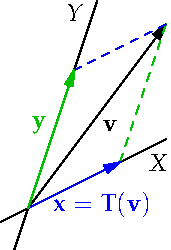
\includegraphics{orth-nonproj}
\end{defn}

\begin{example}{}{proj}
$A=\frac 15\begin{smatrix}
6&-2\\3&-1
\end{smatrix}$ is a projection matrix with $\cR(A)=\Span\stwovec 21$ and $\cN(A)=\Span\stwovec 13$.\smallbreak
Indeed, it is straightforward to describe all projection matrices in $M_2(\R)$. There are three cases:
\begin{enumerate}
  \item $A=I$ is the identity matrix: $\cR(A)=\R^2$ and $\cN(A)=\{\V0\}$;
  \item $A=0$ is the zero matrix: $\cR(A)=\{\V0\}$ and $\cN(A)=\R^2$;
  \item Choose \emph{distinct} subspaces $\cR(A)=\Span\stwovec ab$ and $\cN(A)=\Span\stwovec cd$, then
  \[A=\frac 1{ad-bc}\twovec ab(d\ -c)=\frac 1{ad-bc}\begin{pmatrix}
  ad&-ac\\bd&-bc
  \end{pmatrix}\]
  Think about why this last does what we claim.
\end{enumerate}
\end{example}

It should be clear that every projection $\rT$ has (at most) two eigenspaces:
\begin{itemize}
  \item $\cR(\rT)$ is an eigenspace with eigenvalue 1
  \item $\cN(\rT)$ is an eigenspace with eigenvalue 0
\end{itemize}
If $V$ is finite-dimensional and $\rho,\eta$ are bases of $\cR(T)$, $\cN(T)$ respectively, then the matrix of $\rT$ with respect to $\rho\cup\eta$ has block form
\[[\rT]_{\rho\cup\eta} =\left(\begin{array}{c|c}
I&0\\\hline
0&0
\end{array}\right)\]
where $\Rank I=\Rank\rT$. In particular, every finite-dimensional projection is diagonalizable.
\goodbreak

\begin{lemm}{}{projnotorth}
$\rT\in\cL(V)$ is a projection if and only if $\rT^2=\rT$.
\end{lemm}

\begin{proof}
Throughout, assume $\vr\in\cR(\rT)$ and $\vn\in\cN(\rT)$.\smallbreak
$(\Rightarrow)$\quad Since every vector in $V$ has a unique representation $\vv=\vr+\vn$, simply compute
\[\rT^2(\vv)=\rT\bigl(\rT(\vr+\vn)\bigr)=\rT(\vr)=\vr=\rT(\vv)\]
$(\Leftarrow)$\quad Suppose $\rT^2=\rT$. Note first that if $\vr\in\cR(\rT)$, then $\vr=\rT(\vv)$ for some $\vv\in V$, whence
\[\rT(\vr)=\rT^2(\vv)=\rT(\vv)=\vr\tag{$\dag$}\]
Thus $\rT$ is the identity on $\cR(\rT)$. Moreover, if $\vx\in\cR(\rT)\cap\cN(\rT)$, ($\dag$) says that $\vx=\rT(\vx)=\V0$, whence
\[\cR(\rT)\cap\cN(\rT)=\{\V0\}\]
and so $\cR(\rT)\oplus\cN(\rT)$ is a well-defined \emph{subspace} of $V$.\footnotemark To finish things off, let $\vv\in V$ and observe that
\[\rT\bigl(\vv-\rT(\vv)\bigr)=\rT(\vv)-\rT^2(\vv)=\V0\implies \vv-\rT(\vv)\in\cN(\rT)\]
so that $\vv=\rT(\vv)+\bigl(\vv-\rT(\vv)\bigr)$ is a decomposition into $\cR(\rT)$- and $\cN(\rT)$-parts. We conclude that $V=\cR(\rT)\oplus\cN(\rT)$ and that $\rT$ is a projection.
\end{proof}

\footnotetext{In finite dimensions, the rank--nullity theorem and dimension counting finishes the proof here without having to proceed further:
\[\dim(\cR(\rT)\oplus \cN(\rT))=\Rank\rT+\Null\rT=\dim V\implies \cR(\rT)\oplus \cN(\rT)=V\]}

\goodbreak




Thus far the discussion hasn't had anything to do with inner products\ldots

\begin{defn}{}{}
An \emph{orthogonal projection} is a projection $\rT\in\cL(V)$ on an inner product space for which we additionally have
\[\cN(\rT)=\cR(\rT)^\perp\quad\text{and}\quad \cR(\rT)=\cN(\rT)^\perp\]
Alternatively, given $V=W\oplus W^\perp$, the \emph{orthogonal projection $\pi_W$} is the projection along $W^\perp$ onto $W$: that is
\[\cR(\pi_W)=W\quad\text{and}\quad \cN(\pi_W)=W^\perp\]
The complementary orthogonal projection $\pi_W^\perp=\I-\pi_W$ has $\cR(\pi_W^\perp)=W^\perp$ and $\cN(\pi_W^\perp)=W$.
\end{defn}

\begin{example*}{\ref{ex:proj} continued}{}
The identity and zero matrices are both $2\times 2$ orthogonal projection matrices, while those of type 3 are orthogonal if $\stwovec ab\cdot\stwovec cd=0$: we obtain
\[A=\frac 1{a^2+b^2}\twovec ab(a\ b)=\frac 1{a^2+b^2}\begin{pmatrix}
a^2&ab\\ab&b^2
\end{pmatrix}\]
More generally, if $W\le\F^n$ has orthonormal basis $\{\vect{\vw}{k}\}$, then the matrix of $\pi_W$ is $\sum_{j=1}^k\vw_j\vw_j^*$.
\end{example*}

\goodbreak

\begin{thm}{}{}
A projection $\rT\in\cL(V)$ is orthogonal if and only if it is self-adjoint $\rT=\rT^*$. 
\end{thm}
  
\begin{proof}
($\Rightarrow$)\quad By assumption, $\cR(\rT)$ and $\cN(\rT)$ are orthogonal subspaces. Letting $\vx,\vy\in V$ and using subscripts to denote $\cR(\rT)$- and $\cN(\rT)$-parts, we see that
\[\ip{\vx,\rT(\vy)}=\ip{\vx_r+\vx_n,\vy_r}=\ip{\vx_r,\vy_r+\vy_n}=\ip{\rT(\vx),\vy} \implies \rT^*=\rT\]
($\Leftarrow$)\quad Suppose $\rT$ is a self-adjoint projection. By the fundamental subspaces theorem,
\[\cN(\rT)=\cN(\rT^*)=\cR(\rT)^\perp\]
Since $\rT$ is a projection already, we have $V=\cR(\rT)\oplus\cN(\rT)= \cR(\rT)\oplus \cR(\rT)^\perp$, from which 
\[\cR(\rT)=\bigl(\cR(\rT)^\perp\bigr)^\perp=\cN(\rT)^\perp\tag*{\qedhere}\]
\end{proof}
 

The language of projections allows us to rephrase the Spectral Theorem.
  
\begin{thm}{Spectral Theorem, mk.\,II}{}
Let $V$ be a finite-dimensional complex/real inner product space and $\rT\in\cL(V)$ be normal/self-adjoint with spectrum $\{\lambda_1,\ldots,\lambda_k\}$ and corresponding eigenspaces $E_1,\ldots,E_k$. Let $\pi_j\in\cL(V)$ be the orthogonal projection onto $E_j$. Then:
\begin{enumerate}
  \item $V=E_1\oplus \cdots\oplus E_k$ is a direct sum of orthogonal subspaces, in particular, $E_j^\perp$ is the direct sum of the remaining eigenspaces.
  \item $\pi_i\pi_j=0$ if $i\neq j$.
  \item (Resolution of the identity)\quad $\I_V=\pi_1+\cdots+\pi_k$
  \item (Spectral decomposition)\quad $\rT=\lambda_1\pi_1+\cdots+\lambda_k\pi_k$
\end{enumerate}
\end{thm}

\begin{proof}
\begin{enumerate}
  \item $\rT$ is diagonalizable and so $V$ is the direct sum of the eigenspaces of $\rT$. Since $\rT$ is normal, the eigenvectors corresponding to distinct eigenvalues are orthogonal, whence the eigenspaces are mutually orthogonal. In particular, this says that
  \[\hat E_j:=\bigoplus_{i\neq j}E_i\le E_j^\perp\]
  Since $V$ is finite-dimensional, we have $V=E_j\oplus E_j^\perp$, whence
  \[\dim \hat{E_j}=\sum\limits_{i\neq j}\dim E_i=\dim V-\dim E_j=\dim E_j^\perp \implies \hat E_j=E_j^\perp\]
  \item This is clear by part 1, since $\cN(\pi_j)=E_j^\perp=\hat E_j$.
  \item Write $\vx=\sum_{j=1}^k\vx_j$ where each $\vx_j\in E_j$. Then $\pi_j(\vx)=\vx_j$: now add\ldots
  \item $\rT(\vx)=\sum_{j=1}^k\rT(\vx_j)=\sum_{j=1}^k\lambda_j\vx_j=\sum_{j=1}^k\lambda_j\pi_j(\vx)$.\qedhere
\end{enumerate}
\end{proof}

\goodbreak


\begin{examples}{}{}
We verify the resolution of the identity and the spectral decomposition; for clarity, we index projections and eigenspaces by eigenvalue rather than the natural numbers.
\begin{enumerate}
  \item The symmetric matrix $A=\begin{smatrix}
  10&2\\2&7
  \end{smatrix}$ has spectrum $\{6,11\}$ and orthonormal eigenvectors
  \[\vw_6=\frac 1{\sqrt 5}\twovec 1{-2},\qquad \vw_{11}=\frac 1{\sqrt 5}\twovec 21\]
  The corresponding projections therefore have matrices
  \[\pi_6=\vw_6\vw_6^T=\frac 15\twovec 1{-2}(1\ \ -2)
  =\frac 15\begin{pmatrix}
  1&-2\\-2&4
  \end{pmatrix},\qquad
  \pi_{11}=\vw_{11}\vw_{11}^T
  =\frac 15\begin{pmatrix}
  4&2\\2&1
  \end{pmatrix}\]
  from which the resolution of the identity and the spectral decomposition are readily verified:
  \[\pi_6+\pi_{11}=\begin{pmatrix}
1&0\\0&1
  \end{pmatrix}
  \quad\text{and}\quad
  6\pi_6+11\pi_{11}= \frac 15\begin{pmatrix}
  6+44&-12+22\\
  -12+22&24+11
  \end{pmatrix}=A\]
  
  \item The normal matrix $B=\begin{smatrix}
		1+i&1+i\\
		-1-i&1+i
  \end{smatrix}\in M_2(\C)$ has spectrum $\{2,2i\}$ and corresponding
orthonormal eigenvectors
	\[\vw_2=\frac 1{\sqrt 2}\twovec i1,\qquad \vw_{2i}=\frac 1{\sqrt 2}\twovec 1i\]
	The orthogonal projection matrices are therefore
	\[\pi_2=\vw_2\vw_2^*=\frac 12\twovec i1(-i\ \ 1)=\frac 12\begin{pmatrix}
1&i\\-i&1
	\end{pmatrix}
	\qquad \pi_{2i}=\vw_{2i}\vw_{2i}^*=\frac 12\begin{pmatrix}
	1&-i\\i&1
	\end{pmatrix}\]
	from which
	\begin{gather*}
		\pi_2+\pi_{2i}=\begin{pmatrix}
		1&0\\0&1
		\end{pmatrix}\quad\text{and}\quad
		2\pi_2+2i\pi_{2i}=\begin{pmatrix}
		1&i\\-i&1
		\end{pmatrix}+\begin{pmatrix}
		i&1\\-1&i
		\end{pmatrix}=B
	\end{gather*}

	\item The matrix $C=\begin{smatrix}
		0&1&1\\
		1&0&1\\
		1&1&0
	\end{smatrix}$ has spectrum $\{-1,2\}$, an orthonormal eigenbasis
	\[\{\vu,\vv,\vw\} =\left\{\frac 1{\sqrt 3}\threevec 111, \frac 1{\sqrt 2}\threevec 1{-1}0,\frac 1{\sqrt 6}\threevec 11{-2} \right\}\]
	and eigenspaces $E_2=\Span\{\vu\}$ and $E_{-1}=\Span\{\vv,\vw\}$. The orthogonal projections have matrices
	\begin{gather*}
		\pi_2=\vu\vu^T=\frac 13\threevec 111(1\ \ 1\ \ 1)
		=\frac 13\begin{pmatrix}
			1&1&1\\
			1&1&1\\
			1&1&1
		\end{pmatrix}\\
		\begin{aligned}
			\pi_{-1}&=\vv\vv^T+\vw\vw^T
			=\frac 12\threevec 1{-1}0(1\ \ -1\ \ 0)+\frac 16\threevec 11{-2}(1\ \ 1\ \ -2)\\
			&=\frac 12\begin{pmatrix}
				1&-1&0\\
				-1&1&0\\
				0&0&0
			\end{pmatrix}+\frac 16\begin{pmatrix}
				1&1&-2\\
				1&1&-2\\
				-2&-2&4
			\end{pmatrix}
			=\frac 13\begin{pmatrix}
				2&-1&-1\\
				-1&2&-1\\
				-1&-1&2
			\end{pmatrix}
		\end{aligned}
	\end{gather*}
	It is now easy to check the resolution of the identity and the spectral decomposition:
	\[\pi_2+\pi_{-1}=I\quad\text{and}\quad 2\pi_2-\pi_{-1}=C\]
\end{enumerate}
\end{examples}

\vfil\goodbreak

\boldsubsubsection{Orthogonal Projections and Minimization Problems}\phantomsection\label{sec:leastsq}

We finish this section with an important observation that drives much of the application of inner product spaces to other parts of mathematics and beyond. Throughout this discussion, $X$ and $Y$ denote inner product spaces.


\begin{thm}{}{minthm}
Suppose $Y=W\oplus W^\perp$. For any $\vy\in Y$, the orthogonal projection $\pi_W(\vy)$ is the unique element of $W$ which minimizes the distance to $\vy$:
\[\forall\vw\in W,\ \Nm{\vy-\pi_W(\vy)}\le\Nm{\vy-\vw}\]
\end{thm}

\begin{proof}
Apply Pythagoras' Theorem: since $\pi^\perp_W(\vy)=\vy-\pi_W(\vy)\in W^\perp$,\smallbreak

\begin{minipage}[t]{0.7\linewidth}\vspace{-15pt}
	\begin{align*}
	\Nm{\vy-\vw}^2&=\Nm{\vy-\pi_W(\vy)+\pi_W(\vy)-\vw}^2\\
	&=\Nm{\vy-\pi_W(\vy)}^2+\Nm{\pi_W(\vy)-\vw}^2\\
	&\ge \Nm{\vy-\pi_W(\vy)}^2
	\end{align*}
with equality if and only if $\vw =\pi_W(\vy)$.
	\end{minipage}
	\hfill\begin{minipage}[t]{0.29\linewidth}\vspace{-30pt}
	\flushright\href{http://www.math.uci.edu/~ndonalds/math121b/orth-orthproj4.html}{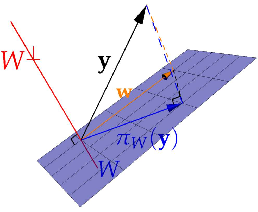
\includegraphics{orth-orthproj4}}
	\end{minipage}\smallbreak
\end{proof}

This set up can be used to compute accurate approximations in many contexts.

\begin{examples}{}{minproj}
\exstart To obtain a quadratic polynomial approximation $p(x)=a+bx+cx^2$ to $e^x$ on the interval $[-1,1]$ we choose to minimize the integral $\int_{-1}^1\nm{e^x-p(x)}^2\,\dx$, namely the squared $L^2$-norm $\Nm{e^x-p(x)}^2$ on $C[-1,1]$. If we let $W=\Span\{1,x,x^2\}$, then the finite-dimensionality of $W$ means that $C[-1,1]=W\oplus W^\perp$. By the Theorem, the solution is $p(x)=\pi_W(e^x)$.
\begin{enumerate}\setcounter{enumi}{1}
    \item[]	To compute this, recall that we have an orthonormal basis for $W$, namely\smallbreak
	
	\begin{minipage}[t]{0.65\linewidth}\vspace{-15pt}
	\[\left\{\tfrac 1{\sqrt 2},\sqrt{\tfrac 32}x,\sqrt{\tfrac 58}(3x^2-1)\right\}\]
		from which
	\begin{align*}
	\textcolor{Green}{p(x)}&=\frac 12\ip{1,e^x}+\frac 32\ip{x,e^x}x+\frac 58(3x^2-1)\ip{3x^2-1,e^x}\\
	&=\frac 12\int_{-1}^1e^x\,\dx +\frac 32x\int_{-1}^1xe^x\,\dx\\
	&\qquad\qquad\qquad+\frac 58(3x^2-1)\int_{-1}^1(3x^2-1)e^x\,\dx\\
	&=\frac 12(e-e^{-1}) +3e^{-1}x +\frac 54(e-7e^{-1})(3x^2-1)\\
	&\approx \textcolor{purple}{1.18+1.10x}+0.179(3x^2-1)\\
	&\approx \textcolor{Green}{1+1.1x+0.537x^2}
	\end{align*}
	\end{minipage}\begin{minipage}[t]{0.35\linewidth}\vspace{0pt}
	\flushright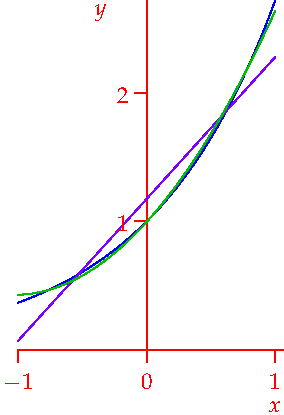
\includegraphics[scale=0.9]{orth-expapprox}
	\end{minipage}\smallbreak	
	The \textcolor{purple}{linear} and \textcolor{Green}{quadratic} approximations to $\textcolor{blue}{y=e^x}$ are drawn. Compare this with the Maclaurin polynomial $e^x\approx 1+x+\frac 12x^2$ from calculus.

	
	\goodbreak
	\item\label{ex:minproj2} The $n\th$ Fourier approximation of a function $f(x)$ is its orthogonal projection onto the finite-dimensional subspace
	\begin{align*}
	W_n&=\Span\{1,e^{ix},e^{-ix},\ldots,e^{inx},e^{-inx}\}\\
	&=\Span\{1,\cos x,\sin x,\cos 2x,\sin 2x,\ldots,\cos nx,\sin nx\}
	\end{align*}
	within $L^2[-\pi,\pi]$, namely
	\begin{align*}
	\mathcal F_n(x)&=\frac 1{2\pi}\sum_{k=-n}^n\ip{f(x),e^{ikx}}e^{ikx}\\
	 &=\frac 1{2\pi}\ip{f(x),1}+\frac 1{\pi}\sum_{k=1}^n\ip{f(x),\cos kx}\cos kx+\ip{f(x),\sin kx}\sin kx
	\end{align*}
	According to the Theorem, this is the unique function in $\mathcal F_n(x)\in W_n$ minimizing the integral
	\[\Nm{f(x)-\mathcal F_n(x)}^2=\int_{-\pi}^\pi\nm{f(x)-\mathcal F_n(x)}^2\,\dx\]
	For example, if $f(x)=\begin{cases}
	1&\text{if }0<x\le\pi\\
	-1&\text{if }-\pi<x\le 0
	\end{cases}$ \space is extended periodically, then
	\[\mathcal F_{2n-1}(x)=\frac 4\pi\sum_{j=1}^n\frac{\sin(2j-1)x}{2j-1}=\frac 4\pi\left(\sin x+\frac{\sin 3x}3+\frac{\sin 5x}5+\cdots+\frac{\sin(2n-1)x}{2n-1} \right)\]
	\begin{center}
	\href{http://www.math.uci.edu/~ndonalds/math121b/orth-fourier.html}{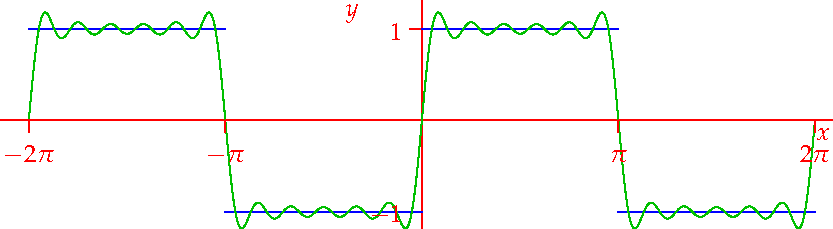
\includegraphics{orth-fourier2}}\\
	\textcolor{blue}{$y=f(x)$} and its eleventh Fourier approximation \textcolor{Green}{$y=\mathcal F_{11}(x)$}
	\end{center}
  
%   \item To obtain a quadratic polynomial approximation $p(x)$ to $e^x$ on the interval $[0,1]$ we might wish to minimize the integral $\int_0^1\nm{e^x-p(x)}^2\,\dx$.\smallbreak
%   
%   The integral is the norm-squared $\Nm{e^x-p(x)}^2$ in the space $C[0,1]$ equipped with the $L^2$ inner product! If we let $W=\Span\{1,x,x^2\}$, then the finite-dimensionality of $W$ means that $C[0,1]=W\oplus W^\perp$. By the theorem, the solution is that $p(x)=\pi_W(e^x)$.\smallbreak
% 	To compute this, recall that we have an orthonormal basis for $W$
% 	\[\beta=\left\{1,\sqrt 3(2x-1),\sqrt{5}(6x^2-6x+1)\right\}\]
% 	from which
% 	\begin{align*}
% 	p(x)&=\ip{1,e^x}+3\ip{2x-1,e^x}(2x-1)+5\ip{6x^2-6x+1,e^x}(6x^2-6x+1)\\
% 	&=\int_0^1e^x\,\dx +3(2x-1)\int_0^1(2x-1)e^x\,\dx+5(6x^2-6x+1)\int_0^1(6x^2-6x+1)e^x\,\dx\\
% 	&=e-1 +3(3-e)(2x-1) +5(7e-19)(6x^2-6x+1)\\
% 	&\approx 1.72+0.84(2x-1)+0.2(6x^2-6x+1)=1.2x^2+0.48x+1.08
% 	\end{align*}
\end{enumerate}
\end{examples}

We'll return to related minimization problems in the next section.

\vfil

\begin{exercises}
\exstart Compute the matrices of the orthogonal projections onto $W$ viewed as subspaces of the standard inner product spaces $\R^n$ or $\C^n$.

\begin{enumerate}\setcounter{enumi}{1}
  \item[]\begin{enumerate}
    \item $W=\Span\twovec 4{-1}$\hfill \text{(b) }\space $W=\Span\left\{\threevec 121,\threevec 10{-1}\right\}$ \hfill \text{(c) }\space
    $W=\Span\left\{\threevec i10,\threevec 1i1\right\}$
    \item[(d)] $W=\Span\left\{\threevec 110,\threevec 121\right\}$\quad (\emph{watch out, these vectors aren't orthogonal!})
	\end{enumerate}
	\goodbreak

	\item For each of the following matrices, compute the projections onto each eigenspace, verify the resolution of the identity and the spectral decomposition.\vspace{-5pt}
	\[\text{(a)}\ \ \begin{pmatrix}
    1&2\\2&1
    \end{pmatrix}
    \qquad
    \text{(b)}\ \ \begin{pmatrix}
    0&-1\\1&0
    \end{pmatrix}
    \qquad
    \text{(c)}\ \ \begin{pmatrix}
    2&3-3i\\3+3i&5
    \end{pmatrix}
    \qquad
    \text{(d)}\ \ \begin{pmatrix}
    2&1&1\\1&2&1\\1&1&2
    \end{pmatrix}
    \]
    \vspace{-5pt}
    (\emph{You should have orthonormal eigenbases from the previous section})
	
	\item If $W$ be a finite-dimensional subspace of an inner product space $V$. If $\rT=\pi_W$ is the orthogonal projection onto $W$, prove that $\I-\rT$ is the orthogonal projection onto $W^\perp$.
	
	\item Let $\rT\in\cL(V)$ where $V$ is finite-dimensional.
	\begin{enumerate}
	  \item If $\rT$ is an orthogonal projection, prove that $\Nm{\rT(\vx)}\le\Nm{\vx}$ for all $\vx\in V$.
	 	\item Give an example of a projection for which the inequality in (a) is \emph{false.}
	 	\item If $\rT$ is a projection for which $\Nm{\rT(\vx)}=\Nm{\vx}$ for all $\vx\in V$, what is $\rT$?
	 	\item If $\rT$ is a projection for which $\Nm{\rT(\vx)}\le\Nm{\vx}$ for all $\vx\in V$, prove that $\rT$ is an \emph{orthogonal} projection.
	\end{enumerate}
	
	\item Let $\rT$ be a normal operator on a finite-dimensional inner product space. If $\rT$ is a projection, prove that it must be an orthogonal projection.
	
	\item\label{exs:lastqn} Let $\rT$ be a normal operator on a finite-dimensional complex inner product space $V$. Use the spectral decomposition $\rT=\lambda_1\pi_1+\cdots+\lambda_k\pi_k$ to prove:
	\begin{enumerate}
	  \item If $\rT^n$ is the zero map for some $n\in\N$, then $\rT$ is the zero map.
	  \item $\rU\in\cL(V)$ commutes with $\rT$ if and only if $\rU$ commutes with each $\pi_j$.
	  \item There exists a normal $\rU\in\cL(V)$ such that $\rU^2=\rT$.
	  \item $\rT$ is invertible if and only if $\lambda_j\neq 0$ for all $j$.
	  \item $\rT$ is a projection if and only if every $\lambda_j=0$ or 1.
	  \item $\rT=-\rT^*$ if and only if every $\lambda_j$ is imaginary.
	\end{enumerate}
	
	\item Find a linear approximation to $f(x)=e^x$ on $[0,1]$ using the $L^2$ inner product.
	
	\item Consider the $L^2$ inner product on $C[-\pi,\pi]$ inner product.
	\begin{enumerate}
	  \item Explain why $\ip{\sin x,x^{2n}}=0$ for all $n$.
	  \item Find linear and \emph{cubic} approximations to $f(x)=\sin x$.\smallbreak
	  (\emph{Feel free to use a computer algebra package to evaluate the integrals}!)
	\end{enumerate}
	
	
	\item Revisit Example \hyperref[ex:minproj2]{\ref*{ex:minproj}.\ref*{ex:minproj2}}
	\begin{enumerate}
	  \item Verify that the general complex ($e^{ikx}$) and real ($\cos kx,\sin kx$) expressions for the Fourier approximation are correct.\smallbreak
	  (\emph{Hint: use Euler's formula $e^{ikx}=\cos kx+i\sin kx$})
	  \item Verify the explicit expression for $\mathcal F_{2n-1}(x)$ when $f(x)$ is the given step-function. What is $\mathcal F_{2n}(x)$ in this case?
% 	  \item Find the $n\th$ Fourier approximation using the interval $[-T,T]$ and the subspace
% 	  \[W_n=\Span\left\{e^{\frac{i\pi kx}T}:-n\le k\le n\right\}=\Span\left\{\cos\frac{k\pi x}T,\sin\frac{k\pi x}T:0\le k\le n\right\}\]
	\end{enumerate}
\end{enumerate}
\end{exercises}
	
	\clearpage


\subsection{The Singular Value Decomposition and the Pseudoinverse}

Given $\rT\in\cL(V,W)$ between finite-dimensional inner product spaces, the overarching concern of this chapter is the existence and computation of bases $\beta,\gamma$ of $V,W$ with two properties:
\begin{itemize}
  \item That $\beta,\gamma$ be \emph{orthonormal,} thus facilitating easy calculation within $V,W$;
  \item That the matrix $[\rT]_\beta^\gamma$ be as simple as possible.
\end{itemize}

We have already addressed two special cases:
\begin{description}
	\item[Spectral Theorem] When $V=W$ and $\rT$ is normal/self-adjoint, $\exists\beta=\gamma$ such that $[\rT]_\beta$ is diagonal.
	\item[Schur's Lemma] When $V=W$ and $p(t)$ splits, $\exists\beta=\gamma$ such that $[\rT]_\beta$ is upper triangular.	
\end{description}

In this section we allow $V\neq W$ and $\beta\neq\gamma$, and obtain a result that applies to any linear map between finite-dimensional inner product spaces.

\begin{example}{}{svd1}
Let $A=\begin{smatrix}
3&1\\
2&-2\\
1&3
\end{smatrix}$ and consider orthonormal bases $\beta=\{\vv_1,\vv_2\}$ of $\R^2$ and $\gamma=\{\vw_1,\vw_2,\vw_3\}$ of $\R^3$ respectively:
\[\beta=\left\{\frac 1{\sqrt 2}\twovec 11,\frac 1{\sqrt 2}\twovec{-1}1\right\},\quad \smash{\gamma=\left\{\frac 1{\sqrt 2}\threevec 101,\frac 1{\sqrt 6}\threevec{-1}{-2}1, \frac 1{\sqrt 3}\threevec 1{-1}{-1}\right\}}\]
Since $A\vv_1=4\vw_1$ and $A\vv_2=2\sqrt 3\vw_2$, whence $[\rL_A]_\beta^\gamma=\begin{smatrix}
4&0\\
0&2\sqrt 3\\
0&0
\end{smatrix}$ is almost diagonal.
\end{example}

Our main result says that such bases always exist.

\begin{thm}{Singular Value Decomposition}{}
Suppose $V,W$ are finite-dimensional inner product spaces and that $\rT\in\cL(V,W)$ has rank $r$. Then:

\begin{enumerate}
  \item There exist orthonormal bases $\beta=\{\vect{\vv}{n}\}$ of $V$ and $\gamma=\{\vect{\vw}{m}\}$ of $W$, and positive scalars $\sigma_1\ge\sigma_2\ge\cdots\ge \sigma_r$ such that
\[\rT(\vv_j)=\begin{cases}
	\sigma_j\vw_j&\text{if }j\le r\\
	\V0&\text{otherwise}
	\end{cases}
	\qquad\text{equivalently}\quad [\rT]_\beta^\gamma=\begin{pmatrix}
	\diag(\sigma_1,\ldots,\sigma_r)&O\\
	O&O
	\end{pmatrix}\]
	\item Any such $\beta$ is an eigenbasis of $\rT^*\rT$, whence the scalars $\sigma_j$ are uniquely determined by $\rT$: indeed
  \[\rT^*\rT(\vv_j)=\begin{cases}
  \sigma_j^2\vv_j&\text{if }j\le r\\
  \V0&\text{otherwise}
  \end{cases}
  \qquad\text{and}\qquad
  \rT^*(\vw_j)=\begin{cases}
  \sigma_j\vv_j&\text{if }j\le r\\
  \V0&\text{otherwise}
  \end{cases}\]
  
	\item If $A\in M_{m\times n}(\F)$ with $\Rank A=r$, then $A=P\Sigma Q^*$ where
  \[\Sigma=[\rL_A]_\beta^\gamma=\begin{pmatrix}
	\diag(\sigma_1,\ldots,\sigma_r)&O\\
	O&O
	\end{pmatrix},\quad P=(\vect{\vw}{m}),\quad Q=(\vect{\vv}{n})\]
	Since the columns of $P,Q$ are orthonormal, these matrices are \emph{unitary.}
\end{enumerate}
\end{thm}

\goodbreak

\begin{defn}{}{}
The numbers $\sigma_1,\ldots,\sigma_r$ are the \emph{singular values} of $\rT$. If $\rT$ is not maximum rank, we have additional zero singular values $\sigma_{r+1}=\cdots=\sigma_{\min(m,n)}=0$.
\end{defn}



\begin{description}
  \item[\normalfont\emph{Freedom of Choice}\quad] While the singular values are uniquely determined, there is often significant freedom regarding the bases $\beta$ and $\gamma$, particularly if any eigenspace of $\rT^*\rT$ has dimension $\ge 2$.
  
  \item[\normalfont\emph{Special Case (Spectral Theorem)}\quad] If $V=W$ and $\rT$ is normal/self-adjoint, we may \emph{choose} $\beta$ to be an eigenbasis of $\rT$, then $\sigma_j$ is the \emph{modulus} of the corresponding eigenvalue (see Exercise \ref{exs:specsingular}).
  
  \item[\normalfont\emph{Rank-one decomposition}\quad] If we write $g_j:V\to\F$ for the linear map $g_j:\vv\mapsto \ip{\vv,\vv_j}$ (recall Riesz's Theorem), then the singular value decomposition says
  \[\rT=\sum_{j=1}^r \sigma_j\vw_jg_j\quad \text{that is}\quad \rT(\vv)=\sum_{j=1}^r \sigma_j\ip{\vv,\vv_j}\vw_j\]
  thus rewriting $\rT$ as a linear combination of rank-one maps ($\vw_jg_j:V\to W$).\\
  For matrices, $g_j$ is simply multiplication by the row vector $\vv_j^*$ and we may write\footnote{Since $\beta$ is orthonormal, it is common to write $\vv_j^*$ for the map $g_j=\langle\quad,\vv_j\rangle$ in general contexts. To those familiar with the \emph{dual space} $V^*=\cL(V,\F)$, the set $\{g_1,\ldots,g_n\}=\{\vv_1^*,\ldots,\vv_n^*\}$ is the \emph{dual basis} to $\beta$. In this course $\vv_j^*$ will only ever mean the \emph{conjugate-transpose} of a \emph{column vector} in $\F^n$. This discussion is part of why physicists write inner products differently!}
	\[A=\sum_{j=1}^r\sigma_j\vw_j\vv_j^*\]
\end{description}

\begin{example*}{\ref{ex:svd1} cont}
We apply the method in the Theorem to $A=\begin{smatrix}
3&1\\
2&-2\\
1&3
\end{smatrix}$.\smallbreak
The symmetric(!) matrix $A^TA=\begin{smatrix}
	14&2\\2&14
  \end{smatrix}$ has eigenvalues $\sigma_1^2=16$, $\sigma_2^2=12$ and orthonormal eigenvectors $\vv_1=\frac 1{\sqrt 2}\stwovec 11$, $\vv_2=\frac 1{\sqrt 2}\stwovec{-1}1$. The singular values are therefore $\sigma_1=4,\sigma_2=2\sqrt 3$. Now compute
  \[\vw_1=\frac 1{\sigma_1}A\vv_1=\frac 1{4\sqrt 2}A\twovec 11=\frac 1{\sqrt 2}\threevec 101,\quad \vw_2=\frac 1{\sigma_2}A\vv_2 =\frac 1{2\sqrt 6}A\twovec{-1}1=\frac 1{\sqrt 6}\threevec{-1}{-2}1\]
  and observe that these are orthonormal. Finally choose $\vw_3=\frac 1{\sqrt 3}\sthreevec 1{-1}{-1}$ to complete the orthonormal basis $\gamma$ of $\R^3$. A singular value decomposition is therefore
  \[
  A=\begin{pmatrix}
  3&1\\2&-2\\1&3
  \end{pmatrix}=P\Sigma Q^*
  =\begin{pmatrix}
  \frac 1{\sqrt 2}&\frac{-1}{\sqrt 6}&\frac 1{\sqrt 3}\\
  0&\frac{-2}{\sqrt 6}&\frac{-1}{\sqrt 3}\\
  \frac 1{\sqrt 2}&\frac{1}{\sqrt 6}&\frac{-1}{\sqrt 3}  
  \end{pmatrix}
  \begin{pmatrix}
  4&0\\0&2\sqrt 3\\0&0
  \end{pmatrix}
  \begin{pmatrix}
  \frac 1{\sqrt 2}&\frac 1{\sqrt 2}\\\frac{-1}{\sqrt 2}&\frac 1{\sqrt 2}
  \end{pmatrix}
	\]
	By expanding the decomposition, $A$ is expressed as the sum of rank-one matrices:
	\[\sigma_1\vw_1\vv_1^T+\sigma_2\vw_2\vv_2^T =4\threevec{\frac 1{\sqrt 2}}0{\frac 1{\sqrt 2}}
	\begin{pmatrix}
	\frac 1{\sqrt 2}&\frac 1{\sqrt 2}
	\end{pmatrix}
	+
	2\sqrt 3\threevec{\frac{-1}{\sqrt 6}}{\frac{-2}{\sqrt 6}}{\frac{1}{\sqrt 6}}
	\begin{pmatrix}
	\frac{-1}{\sqrt 2}&\frac 1{\sqrt 2}
	\end{pmatrix}
  =\begin{pmatrix}
  2&2\\0&0\\2&2
  \end{pmatrix}
  +
  \begin{pmatrix}
  1&-1\\2&-2\\-1&1
  \end{pmatrix}\]
\end{example*}

\goodbreak

\begin{proof}
\begin{enumerate}
  \item Since $\rT^*\rT$ is self-adjoint, the spectral theorem says it has an orthonormal basis of eigenvectors $\beta=\{\vect{\vv}{n}\}$. If $\rT^*\rT(\vv_j)=\lambda_j\vv_j$, then
	\[\ip{\rT(\vv_j),\rT(\vv_k)}=\ip{\rT^*\rT(\vv_j),\vv_k} =\lambda_j\ip{\vv_j,\vv_k} =\begin{cases}
	\lambda_j&\text{if }j=k\\
	0&\text{if }j\neq k
	\end{cases} \tag{$\ast$}\]
	whence every eigenvalue is a non-negative real number: $\lambda_j=\Nm{\rT(\vv_j)}^2\ge 0$.\\
	Since $\Rank\rT^*\rT=\Rank\rT=r$ (Exercise \ref{exs:ranktstart}), exactly $r$ eigenvalues are non-zero; by reordering basis vectors if necessary, we may assume
	\[\lambda_1\ge\cdots\ge\lambda_r>0\]
	If $j\le r$, define $\sigma_j:=\sqrt{\lambda_j}>0$ and $\vw_j:=\frac 1{\sigma_j}\rT(\vv_j)$, then the set $\{\vect{\vw}{r}\}$ is orthonormal ($\ast$). If necessary, extend this to an orthonormal basis $\gamma$ of $W$.
	\item If orthonormal bases $\beta$ and $\gamma$ exist such that $[\rT]_\beta^\gamma=\begin{smatrix}
	\diag(\sigma_1,\ldots,\sigma_r)&O\\
	O&O
	\end{smatrix}$, then $[\rT^*]_\gamma^\beta$ is \emph{essentially the same matrix} just that its dimensions have been reversed:
	\[[\rT^*]_\gamma^\beta=\begin{pmatrix}
	\diag(\sigma_1,\ldots,\sigma_r)&O\\
	O&O
	\end{pmatrix} \implies \rT^*\rT=\begin{pmatrix}
	\diag(\sigma_1^2,\ldots,\sigma_r^2)&O\\
	O&O
	\end{pmatrix}\]
	whence $\rT^*$ and $\rT^*\rT$ are as claimed.
	
% 	\item This is straightforward given part 1.	Observe that
% 	\[\ip{\rT^*(\vw_j),\vv_k}=\ip{\vw_j,\rT(\vv_k)}=\begin{cases}
% 	\sigma_j&\text{if $j=k$ and $k\le r$}\\
% 	0&\text{otherwise}
% 	\end{cases}\]
% 	Since $\beta$ is a basis, it follows that
% 	\[
% 	\rT^*(\vw_j)=\begin{cases}
% 	\sigma_j\vv_j&\text{if $j\le r$}\\
% 	\V0&\text{otherwise}
% 	\end{cases}
% 	\]
% 	We conclude that $\rT^*\rT(\vv_j)=\sigma^2_j\vv_j$.
	\item This is merely part 1 in the context of $\rT=\rL_A\in\cL(\F^n,\F^m)$. The orthonormal bases $\beta,\gamma$ consist of \emph{column vectors} and so the (change of co-ordinate) matrices $P,Q$ are unitary.\qedhere
\end{enumerate}
\end{proof}




\begin{examples}{}{derivpseudo}
\exstart The matrix $A=\begin{smatrix}2&3\\0&2\end{smatrix}$ has $A^TA=\begin{smatrix}
  4&6\\6&13
  \end{smatrix}$ with eigenvalues $\sigma_1^2=16$ and $\sigma_2^2=1$ and orthonormal eigenbasis
	\[\beta=\left\{\frac 1{\sqrt 5}\twovec 1{2},\frac 1{\sqrt 5}\twovec{-2}1\right\}\]
	The singular values are therefore $\sigma_1=4$ and $\sigma_2=1$, from which we obtain
	\[\gamma=\left\{\frac 1{\sigma_1}A\vv_1,\frac 1{\sigma_2}A\vv_2\right\}=\left\{\frac 1{\sqrt 5}\twovec 2{1},\frac 1{\sqrt 5}\twovec{-1}2\right\}\]
	and the decomposition
	\[A=P\Sigma Q^*=
	\begin{pmatrix}
  \frac 2{\sqrt 5}&\frac{-1}{\sqrt 5}\\
  \frac 1{\sqrt 5}&\frac 2{\sqrt 5}  
  \end{pmatrix}
  \begin{pmatrix}
  4&0\\0&1
  \end{pmatrix}
  \begin{pmatrix}
  \frac 1{\sqrt 5}&\frac 2{\sqrt 5}\\
  \frac{-2}{\sqrt 5}&\frac 1{\sqrt 5}  
  \end{pmatrix}\]
  Multiplying out, we may write $A$ as a sum of rank-one matrices
  \[A=\frac 45\twovec 21\begin{pmatrix}
  1&2
  \end{pmatrix}
  +
  \frac 15\twovec{-1}2\begin{pmatrix}
  -2&1
  \end{pmatrix}
  =\frac 45\begin{pmatrix}
  2&4\\
  1&2
  \end{pmatrix}
  +
  \frac 15\begin{pmatrix}
  2&-1\\-4&2
  \end{pmatrix}\]
  
  \goodbreak
  
\begin{enumerate}\setcounter{enumi}{1}
  \item\label{ex:derivpseudo2} The decomposition can be very messy to find in non-matrix situations. Here is a classic example where we simply observe the structure directly.\smallbreak
  The $L^2$ inner product $\ip{f,g}=\int_0^1f(x)g(x)\,\dx$ on $P_2(\R)$ and $P_1(\R)$ admits orthonormal bases
\[\beta=\left\{\sqrt 5(6x^2-6x+1),\sqrt 3(2x-1),1\right\},\qquad \gamma=\left\{\sqrt 3(2x-1),1\right\}\]
Let $\rT=\diff x$ be the derivative operator. The matrix of $\rT$ is already in the required form!
\[[\rT]_\beta^\gamma=\begin{pmatrix}
2\sqrt{15}&0&0\\
0&2\sqrt 3&0
\end{pmatrix}\]
thus $\beta,\gamma$ are suitable bases and the singular values of $\rT$ are $\sigma_1=2\sqrt{15}$ and $\sigma_2=2\sqrt 3$.\smallbreak
Since $\beta,\gamma$ are orthonormal, we could have used the adjoint method to evaluate this directly,
\[[\rT^*\rT]_\beta=([\rT]_\beta^\gamma)^T[\rT]_\beta^\gamma=\begin{pmatrix}
60&0&0\\
0&12&0\\
0&0&0
\end{pmatrix}\implies \sigma_1^2=60,\ \sigma_2^2=12\]
Up to sign, $\{[\vv_1]_\beta,[\vv_2]_\beta,[\vv_3]_\beta\}$ is therefore forced to be the standard ordered basis of $\R^3$, confirming that $\beta$ was the correct basis of $P_2(\R)$ all along! %Of course, both approaches were contingent on having orthonormal bases in the first place\ldots
\end{enumerate}
\end{examples}







% \begin{example}{}{}
% We find the singular value decomposition of the matrix $A=\begin{smatrix}
%   -1&7\\3&4\\7&1
%   \end{smatrix}$.\\[5pt]
%   According to the singular value theorem, we need to compute the orthonormal eigenpairs for
%   \[A^*A=\begin{pmatrix}
%   -1&3&7\\7&4&1
%   \end{pmatrix}\begin{pmatrix}
%   -1&7\\3&4\\7&1
%   \end{pmatrix}
%   =\begin{pmatrix}
%   59&12\\12&66
%   \end{pmatrix}\]
%   When arranged in decreasing order, these are easily seen to be\
%   \[(\vv_1,\lambda_1)=\left(\frac 15\twovec 34,75\right)\quad\text{and}\quad(\vv_2,\lambda_2)=\left(\frac 15\twovec{-4}3,50\right)\]
%   It follows that the singular values are $\sigma_1=\sqrt{75}=5\sqrt 3$ and $\sigma_2=5\sqrt 2$. Now compute the other basis vectors:
%   \[\vu_1:=\frac 1{\sigma_1}A\vv_1=\frac 1{25\sqrt 3}\sthreevec{25}{25}{25}=\frac 1{\sqrt 3}\sthreevec 111,\quad \vu_2:=\frac 1{\sigma_2}A\vv_2=\frac 1{25\sqrt 2}\sthreevec{25}{0}{-25}=\frac 1{\sqrt 2}\sthreevec 10{-1}\]
%   and we take $\vu_3=\frac 1{\sqrt 6}\sthreevec 1{-2}1$ to complete the orthonormal basis $\gamma=\{\vu_1,\vu_2,\vu_3\}$. We conclude that
%   \[A=U\Sigma V=
%   \begin{pmatrix}
%   \frac 1{\sqrt 3}&\frac 1{\sqrt 2}&\frac 1{\sqrt 6}\\
%   \frac 1{\sqrt 3}&0&\frac{-2}{\sqrt 6}\\
%   \frac 1{\sqrt 3}&\frac{-1}{\sqrt 2}&\frac 1{\sqrt 6} 
%   \end{pmatrix}
%   \begin{pmatrix}
%   5\sqrt 3&0\\0&5\sqrt 2\\0&0
%   \end{pmatrix}
%   \begin{pmatrix}
%   \frac 35&\frac{-4}5\\\frac 45&\frac 35 
%   \end{pmatrix}^T\]
% \end{example}



\boldsubsubsection{The Pseudoinverse}

The singular value decomposition of a map $\rT\in\cL(V,W)$ gives rise to a natural map from $W$ back to $V$. This map behaves somewhat like an inverse even when the operator is non-invertible!

\begin{defn}{}{}
Given the singular value decomposition of a rank $r$ map $\rT\in\cL(V,W)$, the \emph{pseudoinverse} of $\rT$ is the linear map $\rT^\dag\in\cL(W,V)$ defined by
  \[\rT^\dag(\vw_j)=\begin{cases}
  \frac 1{\sigma_j}\vv_j&\text{if }j\le r\\
  \V0&\text{otherwise}
  \end{cases}\]
\end{defn}

Restricted to $\Span\{\vect vr\}\to\Span\{\vect wr\}$, the pseudoinverse really does invert $\rT$:

\begin{minipage}[t]{0.34\linewidth}\vspace{0pt}
\begin{gather*}
\rT^\dag\rT(\vv_j)=\begin{cases}
  \vv_j&\text{if }j\le r\\
  \V0&\text{otherwise}
  \end{cases}\\[10pt]
  \rT\rT^\dag(\vw_j)=\begin{cases}
   \vw_j&\text{if }j\le r\\
   \V0&\text{otherwise}
   \end{cases}
\end{gather*}
\end{minipage}\begin{minipage}[t]{0.65\linewidth}\vspace{-2pt}
\flushright$\xymatrix @C0pt @R23pt{
	V \ar@<-0.4ex>@[red][dd]_{\textcolor{red}{\rT}}
		& = 
		& \underbrace{\Span\{\vect vr\}}_{\cN(\rT)^\perp=\cR(\rT^\dag)} \ar@<-0.4ex>@[red]@{-}[d]
		& \oplus
		& \underbrace{\Span\{\vv_{r+1},\ldots,\vv_n\}}_{\cN(\rT)=\cR(\rT^\dag)^\perp} \ar@[red][ddrr]
		&& \{\V0_V\} 
		\\
&&\text{bijection} \ar@<-0.4ex>@[blue][u] \ar@<-0.4ex>@[red][d]&&&\\
	W \ar@<-0.4ex>@[blue][uu]_{\textcolor{blue}{\rT^\dag}}
		& =
		& \overbrace{\Span\{\vect wr\}}^{\cR(\rT)=\cN(\rT^\dag)^\perp} \ar@<-0.4ex>@[blue]@{-}[u]
		& \oplus
		& \overbrace{\Span\{\vw_{r+1},\ldots,\vw_m\}}^{\cR(\rT)^\perp=\cN(\rT^\dag)} \ar@[blue][uurr]
		&& \{\V0_W\}
	}
$
\end{minipage}\smallbreak
Otherwise said, the combinations are \emph{orthogonal projections}: $\rT^\dag\rT=\pi^\perp_{\cN(\rT)}$ and $\rT\rT^\dag=\pi_{\cR(\rT)}$\smallbreak

\pagebreak
Given the singular value decomposition of a matrix $A=P\Sigma Q^*$, its pseudoinverse is that of matrix of $(\rL_A)^\dag$, namely%\footnote{This \emph{isn't} the singular value decomposition of $A^\dag$ since the values $\sigma_1^{-1}\le\sigma_2^{-1}\le\cdots\le\sigma_r^{-1}$ are in the wrong order!}
\[A^\dag=\sum_{j=1}^r\frac 1{\sigma_j}\vv_j\vw_j^*=Q\Sigma^\dag P^* \quad\text{where}\quad\Sigma^\dag=\begin{pmatrix}
	\diag(\sigma_1^{-1},\ldots,\sigma_r^{-1})&O\\
	O&O
	\end{pmatrix}\]
	
% 	Restricted to $\cN(\rT)^\perp=\Span\{\vect{\vv}{r}\}$ we obtain an isomorphism\\[-5pt]
% 	\begin{minipage}[t]{0.55\linewidth}\vspace{-8pt}
% 	\[\at{\rT}{\cN(\rT)^\perp}:\cN(\rT)^\perp\to\cR(\rT)=\Span\{\vect{\vw}{r}\} \]
% 	with inverse $\at{\rT^\dag}{\cR(\rT)}:\cR(\rT)\to\cN(\rT)^\perp$.
% 	Moreover, in terms of orthogonal projections,
% 	\[\rT\rT^\dag=\pi_{\cR(\rT)}\quad\text{and}\quad \rT^\dag \rT=\pi^\perp_{\cN(\rT)}\]
% 	\end{minipage}\begin{minipage}[t]{0.45\linewidth}\vspace{0pt}
% 	\flushright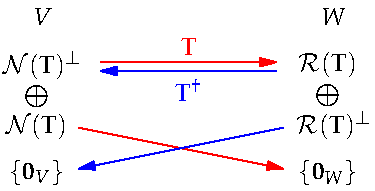
\includegraphics{pseudo-commd}
% 	\end{minipage}

\begin{examples}{}{}
\exstart Again continuing Example \ref{ex:svd1}, $A=\begin{smatrix}
  3&1\\2&-2\\1&3
\end{smatrix}$ has pseudoinverse
  \begin{align*}
  A^\dag&=\frac 1{\sigma_1}\vv_1\vw_1^*+\frac 1{\sigma_2}\vv_2\vw_2^*\\
  &=\frac 1{4\sqrt 2\sqrt 2}\twovec 11(1\ 0\ 1) +\frac 1{2\sqrt 3\sqrt 2\sqrt 6}\twovec{-1}1(-1\ -2\ 1)\\
  &=\frac 18\begin{pmatrix}
  1&0&1\\1&0&1
  \end{pmatrix}+\frac 1{12}\begin{pmatrix}
  1&2&-1\\-1&-2&1
  \end{pmatrix}
  =\frac 1{24}
  \begin{pmatrix}
  5&4&1\\1&-4&5
  \end{pmatrix}
  \end{align*}
  which is exactly what we would have found by computing $A^\dag=Q\Sigma^\dag P^*$. Observe that
  \[A^\dag A=
  \begin{pmatrix}
  1&0\\0&1
  \end{pmatrix}\quad\text{and}\quad
  AA^\dag=\frac 13
  \begin{pmatrix}
  2&1&1\\1&2&1\\1&1&2
  \end{pmatrix}\]
  are the orthogonal projection matrices onto the spaces $\cN(A)^\perp=\Span\{\vv_1,\vv_2\}=\R^2$ and $\cR(A)=\Span\{\vw_1,\vw_2\}\le\R^3$ respectively. Both spaces have dimension 2, since $\Rank A=2$.
%    It also easy to check that
%   \[A(A^TA)^{-1}A^T=AA^\dag\]
% 	in accordance with our discussion of least-squares problems.
	
\begin{enumerate}\setcounter{enumi}{1}	
	\item %Finally we check that the pseudoinverse of the derivative behaves roughly as expected.\smallbreak
The pseudoinverse of $\rT=\diff x:P_2(\R)\to P_1(\R)$, as seen in Example \hyperref[ex:derivpseudo2]{\ref*{ex:derivpseudo}.\ref*{ex:derivpseudo2}}, maps
\begin{gather*}
\rT^\dag(\sqrt 3(2x-1))=\frac 1{2\sqrt{15}}\sqrt 5(6x^2-6x+1) =\frac 1{2\sqrt 3}(6x^2-6x+1)\\
\rT^\dag(1)=\frac 1{2\sqrt 3}\sqrt 3(2x-1)=x-\frac 12\\
\begin{aligned}
\implies \rT^\dag(a+bx)&=\rT^\dag\left(a+\frac b2+\frac b{2\sqrt 3}\sqrt 3(2x-1)\right)\\
&=\left(a+\frac b2\right)\left(x-\frac 12\right)+\frac b{12}(6x^2-6x+1)\\
&=\frac b2x^2+ax-\frac a2-\frac b6
\end{aligned}
\end{gather*}
The pseudoinverse of `differentiation' therefore returns a particular choice of anti-derivative, namely the unique anti-derivative of $a+bx$ lying in $\Span\{\sqrt 5(6x^2-6x+1),\sqrt 3(2x-1)\}$.
\end{enumerate}
	
\end{examples}

% \begin{example}{}{}
% If $T=L_A$ where $A=\begin{smatrix}
%   -1&7\\3&4\\7&1
%   \end{smatrix}$, then we have pseudoinverse
%   \[T^\dag:=\frac 1{\sigma_1}\vv_1\vu_1^*+\frac 1{\sigma_2}\vv_2\vu_2^*\]
%   which has matrix
%   \[A^\dag=\frac 1{5\sqrt 3\cdot 5\cdot\sqrt 3}\twovec 34(1\ 1\ 1) +\frac 1{5\sqrt 2\cdot 5\cdot\sqrt 2}\twovec{-4}3(1\ 0\ -1) =\frac 1{150}
%   \begin{pmatrix}
%   -6&6&18\\17&8&-1
%   \end{pmatrix}\]
%   It is easy to check that
%   \[A^\dag A=\begin{pmatrix}
%   1&0\\0&1
%   \end{pmatrix},
%   \quad\text{and}\quad
%   AA^\dag=\frac 16\begin{pmatrix}
%   5&2&-1\\2&2&2\\-1&2&5
%   \end{pmatrix}\]
%   The first result is unsurprising: since $T$ has rank 2 the restriction $T:\R^2\to\cR(T)$ is a isomorphism!\\
%   Finally, observe that $TT^\dag=\vu_1\vu_1^*+\vu_2\vu_2^*=\pi_{\vu_1}+\pi_{\vu_2}$ is precisely the \emph{orthogonal projection} onto $\cR(T)=\Span\{\vu_1,\vu_2\}$: indeed, given $A$ as above, it is easy to check that
%   \[A(A^TA)^{-1}A^T=AA^\dag\]
%   is the projection matrix onto the column space of $A$, as discussed in Theorem \ref{thm:leastsq}.
%   we see that \[A(A^TA)^{-1}A^T=U\Sigma V(V^T\Sigma^TU^TU\Sigma V)^{-1}V^T\Sigma^TU^T= U\begin{smatrix}
%   1&0&0\\0&1&0\\0&0&0
%   \end{smatrix}U^T=AA^\dag\]
% \end{example}


% \begin{itemize}
%   \item : the closest vector $\vr\in\cR(T)$ to a given $\vu\in U$ is $\vr:=TT^\dag(\vu)$.
%   \item In matrix language, if $A\in M_{m\times n}(\F)$ has rank $n$, then,
%   \[A^\dag=(A^*A)^{-1}A^*\]
%   In particular, if $A\vx=\vb$ is an overdetermined system of linear equations, then $A^\dag A=I_n$ and $AA^\dag=\pi_{R(A)}$, whence $\vx=A^\dag\vb$ is the unique least-squares solution to $A\vx=\vb$: it is the unique vector minimizing the distance $\Nm{A\vx-\vb}$.
% \end{itemize}
% 
% In the above example, for instance, take $\vb=\sthreevec 100$ and consider the overdetermined system
% \[\begin{cases}
% -x+7y=1\\
% 3x+4y=0\\
% 7x+y=0
% \end{cases} \quad\leftrightsquigarrow A\vx=\vb\]
% The unique least-squares solution is
% \[\vx=A^\dag\vb=\frac 1{150}
%   \begin{pmatrix}
%   -6&6&18\\17&8&-1
%   \end{pmatrix}\threevec 100 =\frac 1{150}\twovec{-6}{17} \implies A\vx=\threevec{5/6}{2/6}{-1/6}\]

\vfil\vfil

\begin{exercises}
\exstart\label{exs:pseudo1} Find the ingredients $\beta,\gamma$ and the singular values for each of the following:
\begin{enumerate}\setcounter{enumi}{1}
  \item[]\begin{enumerate}
    \item $\rT\in\cL(\R^2,\R^3)$ where $\rT\stwovec xy=\sthreevec x{x+y}{x-y}$
    \item $\rT:P_2(\R)\to P_1(\R)$ and $\rT(f)=f''$ where $\ip{f,g}:=\int_0^1f(x)g(x)\,\dx$
    \item $V=W=\Span\{1,\sin x,\cos x\}$ and $\ip{f,g}=\int_0^{2\pi}f(x)g(x)\,\dx$, with $\rT(f)=f'+2f$
  \end{enumerate}
  
  \goodbreak
  
  \item\label{exs:pseudo2} Find a singular value decomposition of each of the matrices:
  \begin{enumerate}
    \item $\begin{pmatrix}
    1&1\\1&1\\-1&-1
    \end{pmatrix}$\qquad
    (b)\ \ $\begin{pmatrix}
    1&0&1\\1&0&-1
    \end{pmatrix}$\qquad
    (c)\ \ $\begin{pmatrix}
    1&1&1\\1&-1&0\\1&0&-1
    \end{pmatrix}$
  \end{enumerate}
  
  \item Find an explicit formula for $\rT^\dag$ for each map in Exercise \hyperref[exs:pseudo1]{1}.
  
  \item Find the pseudoinverse of each of the matrix in Exercise \ref{exs:pseudo2}.
  
  \item Suppose $A=P\Sigma Q^*$ is a singular value decomposition.
  \begin{enumerate}
    \item Describe a singular value decomposition of $A^*$.
    \item Explain why $A^\dag=Q\Sigma^\dag P^*$ \emph{isn't} a singular value decomposition of $A^\dag$; what would be the correct decomposition?   	(\emph{Hint: what is wrong with $\Sigma^\dag$?})
  \end{enumerate}
  
  \item Suppose $\rT:V\to W$ is written according to the singular value theorem. Prove that $\gamma$ is a basis of eigenvectors of $\rT\rT^*$ with the \emph{same} non-zero eigenvalues as $\rT^*\rT$, including repetitions.
  
  \item\label{exs:specsingular}\begin{enumerate}
    \item Suppose $\rT=\cL(V)$ is normal. Prove that each $\vv_j$ in the singular value theorem may be chosen to be an eigenvector of $\rT$ and that $\sigma_j$ is the \emph{modulus} of the corresponding eigenvalue.
    \item Let $A=\begin{smatrix}
    0&1\\1&0
    \end{smatrix}$. Show that \emph{any} orthonormal basis $\beta$ of $\R^2$ satisfies the singular value theorem. What is $\gamma$ here? What is it about the \emph{eigenvalues} of $A$ that make this possible?\smallbreak
    (\emph{Even when $\rT$ is self-adjoint, the vectors in $\beta$ need not also be eigenvectors of $\rT$!})
  \end{enumerate}
  
  \item\label{exs:ranktstart} In the proof of the singular value theorem we claimed that $\Rank \rT^*\rT=\Rank\rT$. Verify this by checking explicitly that $\cN(\rT^*\rT)=\cN(\rT)$.\smallbreak
  (\emph{This is circular logic if you use the decomposition, so you must do without!})
  

  
 
  \item Let $V,W$ be finite-dimensional inner product spaces and $\rT\in\cL(V,W)$. Prove:
  \begin{enumerate}
    \item $\rT^*\rT\rT^\dag=\rT^\dag\rT\rT^*=\rT^*$.\\
    (\emph{Hint: evaluate on the basis $\gamma=\{\vect wm\}$ in the singular value theorem})
    \item If $\rT$ is injective, then $\rT^*\rT$ is invertible and $\rT^\dag=(\rT^*\rT)^{-1}\rT^*$.
    \item If $\rT$ is surjective, then $\rT\rT^*$ is invertible and $\rT^\dag=\rT^*(\rT\rT^*)^{-1}$.
  \end{enumerate}
  
  \item Consider the equation $\rT(\vx)=\vb$, where $\rT$ is a linear map between finite-dimensional inner product spaces. A \emph{least-squares solution} is a vector $\vx$ which minimizes $\Nm{\rT(\vx)-\vb}$.
  \begin{enumerate}
    \item Prove that $\vx_0=\rT^\dag(\vb)$ is a least-squares solution and that any other has the form $\vx_0+\vn$ for some $\vn\in\cN(\rT)$.\\
		(\emph{Hint: Theorem \ref{thm:minthm} says that $\vx_0$ is a least-squares solution if and only if $\rT(\vx_0)=\pi_{\cR(\rT)}(\vb)$})
    \item Prove that $\vx_0=\rT^\dag(\vb)$ has smaller norm than any other least-squares solution.
		\item If $\rT$ is injective, prove that $\vx_0=\rT^\dag(\vb)$ is the unique least-squares solution.
	\end{enumerate}

	
% 	\item For the following systems, find the minimal norm solution to the first and the vector which comes closest to solving the second:
% 	\[\begin{cases}
% 		-x+7y=6\\
% 		3x+4y=7\\
% 		7x+y=8
% 		\end{cases}
% 		\qquad\qquad
% 		\begin{cases}
% 		-x+7y=1\\
% 		3x+4y=0\\
% 		7x+y=0
% 		\end{cases}\]
		
	\item Find the minimal norm solution to the first system, and the least-squares solution to the second:
	\[\begin{cases}
		3x+2y+z=9\\
		x-2y+3z=3
		\end{cases}
		\qquad\qquad
		\begin{cases}
		3x+y=1\\
		2x-2y=0\\
		x+3y=0
		\end{cases}\]
\end{enumerate}
\end{exercises}

\clearpage

% \boldsubsubsection{Linear Regression and least-squares problems (non-examinable)}
% 
% Recall Exercise 8. The vector $\vx=A^\dag\vb$ is often known as a \emph{least-squares solution}\footnote{This is something of a misnomer; least-squares solutions are typically most useful when the equation has no solutions and we want to get as close as we can to a solution.} to the linear equation $A\vx=\vb$, since to minimize the (squared-)norm $\Nm{A\vx-\vb}^2$ means minimizing a sum of squares. 
% 
% \begin{defn}{}{}
% Suppose $\rT\in\cL(X,Y)$ and $\vy\in Y$. A \emph{least-squares solution} to the linear equation $\rT(\vx)=\vy$ is any vector $\vx_0\in X$ which minimizes $\Nm{\rT(\vx)-\vy}$.
% \end{defn}
% 
% In a common special situation, there is a unique least-squares solution.
% 
% \begin{thm}{}{}
% Suppose $X,Y$ are finite-dimensional and that $\rT\in\cL(X,Y)$ is injective. Then the unique least squares solution to $\rT(\vx)=\vy$ is given by the pseudoinverse
% \[\vx_0=\rT^\dag(\vy)=(\rT^*\rT)^{-1}\rT(\vy)\]
% \end{thm}
% 
% \begin{proof}
% By Theorem \ref{thm:minthm}, $\vx_0$ is a least-squares solution if and only if
% \[\rT(\vx_0)=\pi_{\cR(\rT)}(\vy)=\rT\rT^\dag(\vy)\]
% Since $\rT$ is injective, it follows that $\vx_0=\rT^\dag(\vy)$. Exercise 7 gives the alternative expression.
% \end{proof}
% 
% Provided $X,Y$ are finite-dimensional, problem 8 shows that $\vx=\rT^\dag(\vy)$ is a least-squares solution.
% 
% If $\vy\in\cR(\rT)$, these are simply solutions: plainly $\rT(\vx_0)=\vy$ minimizes $\Nm{\vy-\rT(\vx_0)}$.\smallbreak
% Otherwise, we want $\vx_0$ to come as close as possible to solving $\rT(\vx)=\vy$. With a little simplification, this can be attacked using a general method.
% 
% \begin{itemize}
%   \item If $Y=\cR(\rT)\oplus \cR(\rT)^\perp$, the Theorem says that $\rT(\vx_0)=\pi_{\cR(\rT)}(\vy)$: equivalently
%   \[\vy-\rT(\vx_0)\in\cR(\rT)^\perp\]
%   \item Additionally, if $\rT$ has an adjoint, the Fundamental Subspaces Theorem says that $\vx_0$ is a least-squares solution if and only if
%   \[
% 	\vy-\rT(\vx_0)\in \cN(\rT^*) \iff \rT^*\rT(\vx_0)=\rT^*(\vy)
% 	\]
% \end{itemize}
% These conditions are certainly met when $X,Y$ are finite-dimensional.
% 
% \begin{thm}{}{}
% Suppose $X,Y$ are finite-dimensional and $\rT\in\cL(X,Y)$. Then:
% \begin{enumerate}
%   \item $\Rank\rT^*\rT=\Rank\rT=\Rank\rT^*$.
%   \item $\rT^*\rT$ and $\rT^*$ have the same range and so $\rT^*\rT(\vx_0)=\rT^*(\vy)$ always has at least one solution.
%   \item If $\Rank\rT=\dim X$ (equivalently $\Null\rT=0$), then $\rT(\vx)=\vy$ has a unique least-squares solution $\vx_0=(\rT^*\rT)^{-1}\rT^*(\vy)$. Moreover, the orthogonal projection onto $\cR(\rT)$ is
%   \[\pi_{\cR(\rT)}=\rT(\rT^*\rT)^{-1}\rT^*\]
% \end{enumerate}
% \end{thm}
% 
% \goodbreak
% 
% \begin{proof}
% \begin{enumerate}
%   \item $\Rank\rT^*=\Rank\rT$ holds for any maps. By the rank--nullity theorem, it therefore suffices to check that $\rT^*\rT$ and $\rT$ have the same nullspace:
% 	\begin{gather*}
% 		\rT(\vx)=\V0\implies \rT^*\rT(\vx)=\V0 \quad\text{and,}\\
% 		\rT^*\rT(\vx)=\V0\implies 0=\ip{\rT^*\rT(\vx),\vx}=\ip{\rT(\vx),\rT(\vx)} =\Nm{\rT(\vx)}^2\implies \rT(\vx)=\V0
% 	\end{gather*}
% 	\item This is immediate from part 1.
% 	\item If $\Rank \rT=\dim V$, then $\rT^*\rT$ is invertible; $\vx_0$ is a least-squares solution if and only if
% 	\[\rT^*\rT(\vx_0)=\rT^*(\vy)\iff\vx_0=(\rT^*\rT)^{-1}\rT^*(\vy)\]
% 	In such a case, $\pi_{\cR(\rT)}(\vy)=\rT(\vx_0)=\rT(\rT^*\rT)^{-1}\rT^*(\vy)$.\hfill\qedhere
% \end{enumerate}
% \end{proof}
% 
% Least-squares problems are often phrased in terms of matrices: when $\rT=\rL_A$ for some $A\in M_{m\times n}(\F)$. Equivalently, we consider a system of linear equations.

% \begin{example}{}{}
% Find the unique least-squares solution to the overdetermined system
% \[\left\{\begin{array}{r@{\hspace{4pt}}c@{\hspace{4pt}}l}
% x_1+3x_2&=&5\\
% x_2&=&1\\
% x_1+2x_2&=&1
% \end{array}\right.\leftrightsquigarrow\  A\vx=\vy\quad\text{where}\quad
% A=\begin{pmatrix}
% 1&3\\
% 0&1\\
% 1&2
% \end{pmatrix},\ \vy=\threevec 511,\ X=\R^2,\ Y=\R^3\]
% The system does not have a explicit solution. Since $\Rank A=2=\dim X$, we may apply the Theorem
% \begin{align*}
% (A^TA)^{-1}A^T&=
% \left[
% \begin{pmatrix}
% 1&0&1\\
% 3&1&2
% \end{pmatrix}\begin{pmatrix}
% 1&3\\
% 0&1\\
% 1&2
% \end{pmatrix}
% \right]^{-1}
% \begin{pmatrix}
% 1&0&1\\
% 3&1&2
% \end{pmatrix}
% =\begin{pmatrix}
% 2&5\\
% 5&14
% \end{pmatrix}^{-1}
% \begin{pmatrix}
% 1&0&1\\
% 3&1&2
% \end{pmatrix}\\
% &
% =\frac 13
% \begin{pmatrix}
% 14&-5\\
% -5&2
% \end{pmatrix}
% \begin{pmatrix}
% 1&0&1\\
% 3&1&2
% \end{pmatrix} 
% =\frac 13\begin{pmatrix}
% -1&-5&4\\
% 1&2&-1
% \end{pmatrix}\\
% \implies \vx_0&=\frac 13\begin{pmatrix}
% -1&-5&4\\
% 1&2&-1
% \end{pmatrix}\threevec 511 =\twovec{-2}{2}
% \end{align*}
% We can check this explicitly using a little multi-variable calculus: let
% \[f(x_1,x_2)=\Nm{\vy-A\vx}^2= (x_1+3x_2-5)^2+(x_2-1)^2+(x_1+2x_2-1)^2\]
% then $f$ is minimized when
% \[\partials[f]{x_1}=4x_1+10x_2-12=0=\partials[f]{x_2} =10x_1+28x_2-36 \iff \twovec{x_1}{x_2}=\twovec{-2}{2}\]
% Moreover, the orthogonal projection onto the range (column space) of $A$ is left-multiplication by the matrix
% \[\pi_{\cR(A)}=A(A^TA)^{-1}A^T =
% \frac 13\begin{pmatrix}
% 1&3\\
% 0&1\\
% 1&2
% \end{pmatrix}
% \begin{pmatrix}
% -1&-5&4\\
% 1&2&-1
% \end{pmatrix} =\frac 13\begin{pmatrix}
% 2&1&1\\
% 1&2&-1\\
% 1&-1&2
% \end{pmatrix}\]
% which may be verified directly by first finding an orthonormal basis $\left\{\frac 1{\sqrt 2}\sthreevec 101,\frac 1{\sqrt 6}\sthreevec 12{-1}\right\}$ of $\cR(A)$.
% \end{example}

\boldsubsubsection{Linear Regression (non-examinable)}

Given a data set $\{(t_j,y_j):1\le j\le m\}$, we may employ the least-squares method to find a \emph{best-fitting line} $y=c_0+c_1t$; often used to predict $y$ given a value of $t$.\smallbreak
The trick is to minimize the sum of the squares of the \textcolor{Green}{vertical deviations} of the line from the data set.
\[\sum_{j=1}^m\nm{y_j-c_0-c_1t_j}^2=\Nm{\vy-A\vx}^2\quad\text{where}\quad A=\begin{pmatrix}
t_1&1\\
\vdots&\vdots\\
t_m&1
\end{pmatrix}\quad \vx=\twovec{c_1}{c_0}\quad \vy=\threevec{y_1}{\vdots}{y_m} \]
With the indicated notation, we recognize this as a least-squares problem. Indeed if there are at least two distinct $t$-values in the data set, then $\Rank A=2$ is maximal and we have a unique best-fitting line with coefficients given by
\[\twovec{c_1}{c_0}=A^\dag\vy =(A^TA)^{-1}A^T\vy\]


\begin{example}{}{lsq}
Given the data set $\{(0,1),(1,1),(2,0),(3,2),(4,2)\}$, we compute
\begin{align*}
A=\begin{pmatrix}
0&1\\
1&1\\
2&1\\
3&1\\
4&1
\end{pmatrix},\quad \vy=\begin{pmatrix}
1\\1\\0\\2\\2
\end{pmatrix} \implies \vx_0&=\twovec{c_1}{c_0} =(A^TA)^{-1}A^T\vy=\begin{pmatrix}
30&10\\
10&5
\end{pmatrix}^{-1}
\twovec{15}{6} =\frac 3{10}\twovec{1}{2}
\end{align*}
The regression line therefore has equation $y=\frac 3{10}(t+2)$.\smallbreak
The process can be applied more generally to approximate using other functions. To find the best-fitting quadratic polynomial $y=c_0+c_1t+c_2t^2$, we'd instead work with
\begin{gather*}
A=\begin{pmatrix}
t_1^2&t_1&1\\
\vdots&\vdots&\vdots\\
t_m^2&t_m&1
\end{pmatrix}\quad \vx=\threevec{c_2}{c_1}{c_0}\quad \vy=\threevec{y_1}{\vdots}{y_m} \implies \sum_{j=1}^m\nm{y_j-c_0-c_1t-c_2t_j^2}^2 =\Nm{\vy-A\vx}^2
\end{gather*}
Provided we have at least three distinct values $t_1,t_2,t_3$, the matrix $A$ is guaranteed to have rank 3 and there will be a best-fitting least-squares quadratic: in this case
\[y=\frac 1{70}(15t^2-39t+72)\]
This curve and the best-fitting straight line are shown below.
\begin{center}
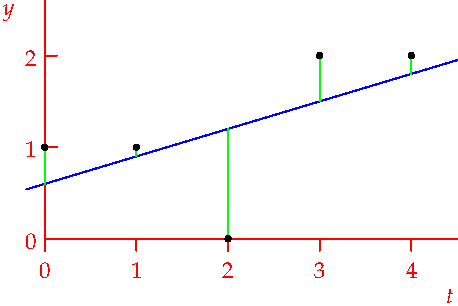
\includegraphics{least-sq-line}
\qquad
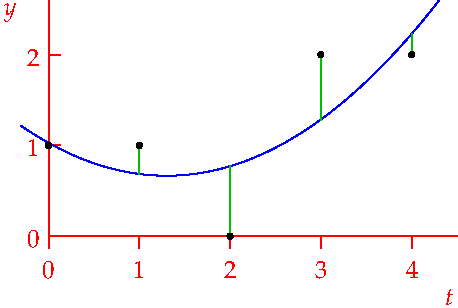
\includegraphics{least-sq-quad}
\end{center}
\end{example}

 %For instance, to find the best-fitting curve of the form $y=ae^t+b$, we would apply the method to
% \[A=\begin{pmatrix}
% e^{t_1}&1\\
% \vdots&\vdots\\
% e^{t_m}&1
% \end{pmatrix}\quad \vx=\twovec{a}{b}\quad \vy=\threevec{y_1}{\vdots}{y_m} \implies \sum_{j=1}^m\nm{y_j-ae^{t_j}-b}^2 =\Nm{\vy-A\vx}^2\]

\begin{tcolorbox}[exercisestyle,title={Optional Problems\quad }]
Use a computer to invert any $3\times 3$ matrices!
\begin{enumerate}
	\item Check the calculation for the best-fitting least-squares quadratic in Example \ref{ex:lsq}.
  
  \item Find the best-fitting least-squares linear and quadratic approximations to the data set
  \[\left\{(1,2),(3,4),(5,7),(7,9),(9,12)\right\}\]
  
  \item Suppose a data set $\{(t_j,y_j):1\le j\le m\}$ has unique regression line $y=ct+d$.
  \begin{enumerate}
    \item Show that the equations $A^TA\vx_0=A^T\vy$ can be written in matrix form
    \[\begin{pmatrix}
    \sum t^2_j&\sum t_j\\
    \sum t_j&m
    \end{pmatrix}\twovec cd =\twovec{\sum t_jy_j}{\sum y_j}\]
    \item Recover the standard expressions from statistics:
    \[c=\frac{\Cov(t,y)}{\sigma^2_t}\ \text{ and }\ d=\cl y-c\cl t\]
    where
    \begin{itemize}
      \item $\displaystyle\cl t=\frac 1m\sum_{j=1}^m t_j$ and $\displaystyle\cl y=\frac 1m\sum_{j=1}^m y_j$ are the \emph{means} (averages),
      \item $\displaystyle\sigma^2_t=\frac 1m\sum_{j=1}^m(t_j-\cl t)^2$ is the \emph{variance},
      \item $\displaystyle\Cov(t,y)=\frac 1m\sum_{j=1}^m(t_j-\cl t)(y_j-\cl y)$ is the \emph{covariance.}
    \end{itemize}
	\end{enumerate}
\end{enumerate}
\end{tcolorbox}

\clearpage

\subsection{Bilinear and Quadratic Forms}

In this section we slightly generalize the idea of an inner product. Throughout, $V$ is a vector space over a field $\F$; it need not be an inner product space and $\F$ can be any field (not just $\R$ or $\C$).

\begin{defn}{}{}
A \emph{bilinear form} $B:V\times V\to\F$ is linear in each entry: $\forall \vv,\vx,\vy\in V,\lambda\in\F$,
  \[B(\lambda\vx+\vy,\vv)=\lambda B(\vx,\vv)+B(\vy,\vv),\qquad B(\vv,\lambda\vx+\vy)=\lambda B(\vv,\vx)+B(\vv,\vy)\]
Additionally, $B$ is \emph{symmetric} if $\forall \vx,\vy\in V$,\ $B(\vx,\vy)=B(\vy,\vx)$.
\end{defn}

\begin{examples}{}{bilinear}
\exstart If $V$ is a \emph{real} inner product space, then the inner product $\ip{\ ,\ }$ is a symmetric bilinear form. Note that a \emph{complex} inner product is \emph{not bilinear!}

\begin{enumerate}\setcounter{enumi}{1}
	\item\label{ex:bilinear1} If $A\in M_n(\F)$, then $B(\vx,\vy):=\vx^TA\vy$ is a bilinear form on $\F^n$. For instance, on $\R^2$,
	\[B(\vx,\vy)=\vx^T\begin{pmatrix}
	1&2\\2&0
	\end{pmatrix}\vy =x_1y_1+2x_1y_2+2x_2y_1\]
	defines a symmetric bilinear form, though not an inner product since it isn't positive definite; for example $B(\vj,\vj)=0$.
% 	
%   \item On the vector space $V=\Z_3^2$ over the finite field $\Z_3=\{0,1,2\}$ of remainders modulo 3, define
%   \[B(\vx,\vy)=\vx^T\begin{pmatrix}
% 	2&0\\1&1
% 	\end{pmatrix}\vy=2x_1y_1+x_2y_1+x_2y_2\]
% 	For instance, $B\left(\stwovec 20,\stwovec 12\right)=1$. This isn't symmetric, since $B\left(\stwovec 12,\stwovec 20\right)=2$.
\end{enumerate}
\end{examples}

As seen above, we often make use of a matrix.

\begin{defn}{}{}
Let $B$ be a bilinear form on a finite-dimensional space with basis $\epsilon=\{\vect{\vv}{n}\}$. The \emph{matrix of $B$ with respect to $\epsilon$} is the matrix $[B]_\epsilon=A\in M_n(\F)$ with $ij^\text{th}$ entry
\[A_{ij}=B(\vv_i,\vv_j)\]
\end{defn}

Given $\vx,\vy\in V$, compute their co-ordinate vectors $[\vx]_\epsilon,[\vy]_\epsilon$ with respect to $\epsilon$, then
\[B(\vx,\vy)=[\vx]_\epsilon^TA[\vy]_\epsilon\]
The set of bilinear forms on $V$ is therefore in bijective correspondence with $M_n(\F)$. Moreover,
\[B(\vy,\vx)=[\vy]_\epsilon^TA[\vx]_\epsilon=\left([\vy]_\epsilon^TA[\vx]_\epsilon\right)^T=[\vx]_\epsilon^TA^T[\vy]_\epsilon\]
Finally, if $\beta$ is another basis of $V$, then an appeal to the change of co-ordinate matrix $Q_\epsilon^\beta$ yields
\[B(\vx,\vy)=[\vx]_\epsilon^TA[\vy]_\epsilon =(Q_\beta^\epsilon[\vx]_\beta)^TA(Q_\beta^\epsilon[\vy]_\epsilon) =[\vx]_\beta^T(Q_\beta^\epsilon)^TAQ_\beta^\epsilon[\vy]_\beta \implies [B]_\beta=(Q_\beta^\epsilon)^T[B]_\epsilon Q_\beta^\epsilon\]
To summarize:

\begin{lemm}{}{}
Let $B$ be a bilinear form on a finite-dimensional vector space.
\begin{enumerate}
  \item If $A$ is the matrix of $B$ with respect to some basis, then every other matrix of $B$ has the form $Q^TAQ$ for some invertible $Q$.
  \item $B$ is symmetric if and only if its matrix with respect to any (and all) bases is symmetric.
\end{enumerate}
\end{lemm}

Naturally, the simplest situation is when the matrix of $B$ is diagonal\ldots
\goodbreak

\begin{examples}{}{}
\exstart Example \hyperref[ex:bilinear1]{\ref*{ex:bilinear}.\ref*{ex:bilinear1}} can be written
\begin{align*}
B(\vx,\vy)&=\vx^T\begin{pmatrix}
1&2\\2&0
\end{pmatrix}\vy =x_1y_1+2x_1y_2+2x_2y_1 =(x_1+2x_2)(y_1+2y_2)-4x_2y_2\\
&=\bigl(x_1+2x_2\quad x_2\bigr)\begin{pmatrix}
1&0\\0&-4
\end{pmatrix}\twovec{y_1+2y_2}{y_2} =\vx^T\begin{pmatrix}
 	1&2\\0&1
\end{pmatrix}^T\begin{pmatrix}
1&0\\0&-4
\end{pmatrix}\begin{pmatrix}
 	1&2\\0&1
\end{pmatrix}\vy %\\
% \implies &[B]_\gamma=\begin{pmatrix}
% 1&0\\0&-4
% \end{pmatrix}\quad\text{where}\quad\gamma=\left\{\twovec 10,\twovec{-2}1\right\}
\end{align*}
If $\epsilon$ is the standard basis, then $[B]_\beta=\begin{smatrix}
1&0\\0&-4
\end{smatrix}$ where $Q_\epsilon^\beta=\begin{smatrix}
 	1&2\\0&1
\end{smatrix}$. It follows that $Q_\beta^\epsilon=\begin{smatrix}
 	1&-2\\0&1
\end{smatrix}$ from which $\beta=\left\{\stwovec 10,\stwovec{-2}1\right\}$ is a diagonalizing basis.
\begin{enumerate}\setcounter{enumi}{1}
  \item In general, we may perform a sequence of \emph{simultaneous} row and column operations to diagonalize \emph{any} symmetric $B$; we require only elementary matrices $E_{ij}^{(\lambda)}$ of type III.\footnotemark For instance:
\begin{align*}
&B(\vx,\vy)=\vx^TA\vy=\vx^T
\begin{pmatrix}
	1&-2&3\\-2&0&4\\3&4&-1
\end{pmatrix}\vy \tag{$A=[B]_\epsilon$ with respect to the standard basis}\\
&E_{21}^{(2)}AE_{12}^{(2)}=\begin{pmatrix}
	1&0&3\\0&-4&10\\3&10&-1
\end{pmatrix} \tag{add twice row 1 to row 2, columns similarly}\\
&E_{31}^{(-3)}E_{21}^{(2)}AE_{12}^{(2)}E_{13}^{(-3)}=\begin{pmatrix}
	1&0&0\\0&-4&10\\0&10&-10
\end{pmatrix} \tag{subtract 3 times row 1 from row 3, etc.}\\
&E_{23}^{(1)}E_{31}^{(-3)}E_{21}^{(2)}AE_{12}^{(2)}E_{13}^{(-3)}E_{32}^{(1)}=\begin{pmatrix}
	1&0&0\\0&6&0\\0&0&-10
\end{pmatrix} \tag{add row 3 to row 2, etc.}
\end{align*}
If $\beta$ is the diagonalizing basis, the the change of co-ordinate matrix is
\[Q_\beta^\epsilon=E_{12}^{(2)}E_{13}^{(-3)}E_{32}^{(1)}
=\begin{pmatrix}
	1&2&0\\0&1&0\\0&0&1
\end{pmatrix}
\begin{pmatrix}
	1&0&-3\\0&1&0\\0&0&1
\end{pmatrix}
\begin{pmatrix}
	1&0&0\\0&1&0\\0&1&1
\end{pmatrix}
=\begin{pmatrix}
	1&-1&-3\\0&1&0\\0&1&1
\end{pmatrix}\]
from which $\beta=\left\{\sthreevec 100,\sthreevec{-1}11,\sthreevec{-3}01\right\}$. If you're having trouble believing this, invert the change of co-ordinate matrix and check that
\[B(\vx,\vy)=(x_1-2x_2+3x_3)(y_1-2y_2+3y_3)+6x_2y_2-10(-x_2+x_3)(-y_2+y_3)\]
\end{enumerate}
\end{examples}

\footnotetext{Recall that $\smash[b]{E_{ij}^{(\lambda)}}$ is the identity matrix with an additional $\lambda$ in the $ij^\text{th}$ entry.
 \begin{itemize}\itemsep0pt\parsep0pt
   \item As a \emph{column} operation (right-multiplication), $A\mapsto A\smash{E_{ij}^{(\lambda)}}$ adds $\lambda$ times the $i^\text{th}$ column to the $j^\text{th}$.
   \item As a \emph{row} operation (left-multiplication), $A\mapsto E_{ji}^{(\lambda)}A=(E_{ij}^{(\lambda)})^TA$ adds $\lambda$ times the $i^\text{th}$ row to the $j^\text{th}$.
 \end{itemize}} 

\textcolor{red}{Warning!} If $\F=\R$ then every symmetric $B$ may be diagonalized by an orthonormal basis (for the usual dot product on $\R^n$). It is \emph{very} unlikely that our algorithm will produce such! The algorithm has two main advantages over the spectral theorem: it is typically faster and it applies to vector spaces over any field. As a disadvantage, it is highly non-unique.

\goodbreak

\begin{example}{}{diagbilinear}
We diagonalize $B(\vx,\vy)=\vx^T\begin{smatrix}1&6\\6&3\end{smatrix}\vy =x_1y_1+6x_1y_2+6x_2y_1+3x_2y_2$ in three ways.
\begin{itemize}
  \item $\begin{smatrix}1&0\\-6&1\end{smatrix}
  \begin{smatrix}1&6\\6&3\end{smatrix}
  \begin{smatrix}1&-6\\0&1\end{smatrix}
  =\begin{smatrix}1&0\\0&-33\end{smatrix}=[B]_\beta$ where $\beta=\left\{\stwovec 10,\stwovec{-6}1\right\}$. This corresponds to 
  \[B(\vx,\vy)=(x_1+6x_2)(y_1+6y_2)-33x_2y_2\]
  \item $\begin{smatrix}1&-2\\0&1\end{smatrix}
  \begin{smatrix}1&6\\6&3\end{smatrix}
  \begin{smatrix}1&0\\-2&1\end{smatrix}
  =\begin{smatrix}-11&0\\0&3\end{smatrix}=[B]_\gamma$ where $\gamma=\left\{\stwovec 1{-2},\stwovec 01\right\}$. This corresponds to 
  \[B(\vx,\vy)=-11x_1y_1+3(2x_1+x_2)(2y_1+y_2)\]
  \item If $\F=\R$, we may apply the spectral theorem to see that $[B]_\eta=\smash[t]{\begin{smatrix}2+\sqrt{37}&0\\0&2-\sqrt{37}\end{smatrix}}$ is diagonal with respect to $\eta=\left\{\stwovec 6{1+\sqrt{37}},\stwovec{-1-\sqrt{37}}6\right\}$. The expression for $B(\vx,\vy)$ in these co-ordinates is disgusting, so we omit it; that $B$ can be diagonalized orthogonally doesn't mean it should be! 
  
%   is an orthogonal eigenbasis, with respect to which $B$ is diagonal
%   \begin{gather*}
%   [B]_\eta=\frac 1{74+2\sqrt{37}}
%   \begin{smatrix}6&1+\sqrt{37}\\-1-\sqrt{37}&6\end{smatrix}
%   \begin{pmatrix}1&6\\6&3\end{pmatrix}
%   \begin{smatrix}6&-1-\sqrt{37}\\1+\sqrt{37}&6\end{smatrix}
%   =\begin{smatrix}2+\sqrt{37}&0\\0&2-\sqrt{37}\end{smatrix}%\\
%   \begin{aligned}
%   B(\vx,\vy)&=(2+\sqrt{37})\frac{(6x_1+(1+\sqrt{37})x_2)(6y_1+(1+\sqrt{37})y_2)}{74+2\sqrt{37}}\\
%   &\qquad\qquad +(2-\sqrt{37})\frac{(6x_2-(1+\sqrt{37})x_1)(6y_2-(1+\sqrt{37})y_1)}{74+2\sqrt{37}}
%   \end{aligned}
  %\end{gather*}

\end{itemize}
\end{example}

\begin{thm}{}{}
Suppose $B$ is a bilinear form of a finite-dimensional space $V$ over $\F$.
\begin{enumerate}
  \item If $B$ is diagonalizable, then it is symmetric.
  \item If $B$ is symmetric and $\F$ does not have characteristic two (see aside), then $B$ is diagonalizable. 
\end{enumerate}
\end{thm}

\begin{proof}
\begin{enumerate}
  \item If $B$ is diagonalizable, $\exists\beta$ such that $[B]_\beta$ is diagonal and thus symmetric.
  \item Suppose $B$ is non-zero (otherwise the result is trivial). We prove by induction on $n=\dim V$.\smallbreak
  If $n=1$, the result is trivial: $B(x,y)=axy$ for some $a\in \F$ is clearly symmetric.\smallbreak
	Fix $n\in\N$ and assume that every non-zero symmetric bilinear form on a dimension $n$ vector space over $\F$ is diagonalizable. Let $\dim V=n+1$. By the discussion below, $\exists \vx\in V$ such that $B(\vx,\vx)\neq 0$. Consider the linear map
\[\rT:V\to\F:\vv\mapsto B(\vx,\vv)\]
Clearly $\Rank\rT=1\implies \dim\cN(\rT)=n$. Moreover, $B$ is symmetric when restricted to $\cN(\rT)$; by the induction hypothesis there exists a basis $\beta$ of $\cN(\rT)$ such that $[\at{B}{\cN(\rT)}]_\beta$ is diagonal. But then $B$ is diagonal with respect to the basis $\beta\cup\{\vx\}$.\qedhere 
\end{enumerate}
\end{proof}



\begin{aside}{}{}
{\bfseries Aside: Characteristic two fields}\quad This means $1+1=0$ in $\F$; this holds, for instance, in the field $\Z_2=\{0,1\}$ of remainders modulo 2. We now see the importance of $\operatorname{char}\F\neq 2$ to the above result.
\begin{itemize}
	\item The proof uses the existence of $\vx\in V$ such that $B(\vx,\vx)\neq 0$. If $B$ is non-zero, $\exists\vu,\vv$ such that $B(\vu,\vv)\neq 0$. If both $B(\vu,\vu)=0=B(\vv,\vv)$, then $\vx=\vu+\vv$ does the job whenever $\operatorname{char}\F\neq 2$:
	\[B(\vx,\vx)=B(\vu,\vv)+B(\vv,\vu)=2B(\vu,\vv)\neq 0\]

	\item To see that the requirement isn't idle, consider $B(\vx,\vy)=\vx^T\begin{smatrix}0&1\\1&0\end{smatrix}\vy$ on the finite vector space $\Z_2^2=\{\stwovec 00,\stwovec 10,\stwovec 01,\stwovec 11\}$ over $\Z_2$. Every element of this space satisfies $B(\vx,\vx)=0$! Perhaps surprisingly, the matrix of $B$ is identical with respect to \emph{any} basis of $\Z_2^2$, whence $B$ is symmetric but non-diagonalizable.
\end{itemize}

% : choose any  and if both $B(\vu,\vu)=0=B(\vv,\vv)$, then $\vx=\vu+\vv$ satisfies
% \[B(\vx,\vx)=2B(\vu,\vv)\neq 0\]
% This is where the characteristic $\neq 2$ condition comes in!
% Why the problem with characteristic 2? Consider $B=\vv^T\begin{smatrix}0&1\\1&0\end{smatrix}\vw$. If we apply our algorithm:
% \begin{align*}
% &E_{12}^{(1)}\begin{pmatrix}
% 	0&1\\1&0
% \end{pmatrix}E_{21}^{(1)}=\begin{pmatrix}
% 	2&1\\1&0
% \end{pmatrix} \tag{add the second row to the first, columns similarly}\\
% &E_{21}^{(-1/2)}E_{12}^{(1)}\begin{pmatrix}
% 	0&1\\1&0
% \end{pmatrix}E_{21}^{(1)}E_{12}^{(-1/2)}=\begin{pmatrix}
% 	2&0\\0&-\frac 12
% \end{pmatrix} \tag{subtract $\frac 12$ row 1 from row 2, etc.}
% \end{align*}
% Since $Q=E_{21}^{(1)}E_{12}^{(-1/2)}= \begin{smatrix}
% 	1&0\\1&1
% \end{smatrix}\begin{smatrix}
% 	1&-\frac 12\\0&1
% \end{smatrix}=\begin{smatrix}
% 	1&-\frac 12\\1&\frac 12
% \end{smatrix}$
% we see that $B$ is diagonal with respect to the basis $\gamma=\left\{\stwovec 11,\stwovec{-1/2}{1/2}\right\}$. If the field has characteristic 2, however, then $\frac 12$ is meaningless! Perhaps surprisingly, the matrix of $B$ is the same with respect to \emph{any} basis of $\Z_2^2$: $B$ is therefore non-diagonalizable!
\end{aside}

\goodbreak


In Example \ref{ex:diagbilinear} notice how the three diagonal matrix representations have something in common: one each of the diagonal entries are positive and negative. This is a general phenomenon:

\begin{thm}{Sylvester's Law of Inertia}{}
Suppose $B$ is a symmetric bilinear form on a real vector space $V$ with diagonal matrix representation $\diag(\lambda_1,\ldots,\lambda_n)$. Then the number of entries $\lambda_j$ which are positive/negative/zero is independent of the diagonal representation.
\end{thm}

\begin{defn}{}{}
The \emph{signature} of a symmetric bilinear form $B$ is the triple $(n_+,n_-,n_0)$ representing how many positive, negative and zero terms are in any diagonal representation. Sylvester's Law says that the signature is an \emph{invariant} of a symmetric bilinear form.
\end{defn}

Positive-definiteness says that a real inner product on an $n$-dimensional space has signature $(n,0,0)$. Practitioners of relativity often work in \emph{Minkowski spacetime}: $\R^4$ equipped with a signature $(1,3,0)$ bilinear form, typically
\[B(\vx,\vy)=\vx^T\begin{pmatrix}
c^2&0&0&0\\
0&-1&0&0\\
0&0&-1&0\\
0&0&0&-1
\end{pmatrix}\vy =c^2x_1y_1-x_2y_2-x_3y_3-x_4y_4\]
where $c$ is the speed of light. Vectors are \emph{time-, space-,} or \emph{light-like} depending on whether $B(\vx,\vx)$ is positive, negative or zero. For instance $\vx=3c^{-1}\ve_1+2\ve_2+2\ve_3+\ve_4$ is light-like.

\begin{proof}
For simplicity, let $V=\R^n$ and write $B(\vx,\vy)=\vx^TA\vy$ where $A$ is symmetric.
\begin{enumerate}
  \item Define $\Rank B:=\Rank A$ and observe this is independent of basis (exercises).
  \item Let $\beta,\gamma$ be diagonalizing bases, ordered according to whether $B$ is \textcolor{red}{positive}, \textcolor{blue}{negative} or \textcolor{Green}{zero}.
  \begin{gather*}
  \beta=\{\textcolor{red}{\vv_1},\ldots,\textcolor{red}{\vv_p}, \textcolor{blue}{\vv_{p+1}},\ldots,\textcolor{blue}{\vv_r}, \textcolor{Green}{\vv_{r+1}},\ldots,\textcolor{Green}{\vv_n}  \}\\
  \gamma=\{\textcolor{red}{\vw_1},\ldots,\textcolor{red}{\vw_q}, \textcolor{blue}{\vw_{q+1}},\ldots,\textcolor{blue}{\vw_r}, \textcolor{Green}{\vw_{r+1}},\ldots,\textcolor{Green}{\vw_n}  \}
  \end{gather*}
  Here $r=\Rank B$ in accordance with part 1: our goal is to prove that $p=q$.
  \item Assume $p<q$, define the matrix $C$ and check what follows:
  \[C=\begin{smatrix}
    \textcolor{red}{\vv_1^T}A\\\vdots\\\textcolor{red}{\vv_p^T}A\\\textcolor{blue}{\vw_{q+1}^T}A\\\vdots\\\textcolor{blue}{\vw_{r}^T}A
    \end{smatrix}\in M_{(r-q+p)\times n}(\R)\]
    \begin{enumerate}
      \item $\Rank C\le r-q+p<r\implies \Null C> n-r$, thus
      \[\exists\vx\in\R^n\text{ such that }C\vx=\V0 \text{ and }\vx\not\in\Span\{\textcolor{Green}{\vv_{r+1}},\ldots,\textcolor{Green}{\vv_n}\}\]
      \item The first $p$ entries of $C\vx=\V0$ mean that $\vx\in\Span\{\textcolor{blue}{\vv_{p+1}},\ldots,\textcolor{blue}{\vv_r}, \textcolor{Green}{\vv_{r+1}},\ldots,\textcolor{Green}{\vv_n}\}$ and so $B(\vx,\vx)<0$. Note how we use part (a) to get a strict inequality here.
      \item Now write $\vx$ with respect to $\gamma$: this time we see that $\vx\in\Span\{\textcolor{red}{\vw_1},\ldots,\textcolor{red}{\vw_q}, \textcolor{Green}{\vw_{r+1}},\ldots,\textcolor{Green}{\vw_n}\}$, whence $B(\vx,\vx)\ge 0$: a contradiction.\qedhere
 		\end{enumerate}
\end{enumerate}
\end{proof}

\goodbreak

\boldsubsubsection{Quadratic Forms \& Diagonalizing Conics}


\begin{defn}{}{}
To every symmetric bilinear form $B:V\times V\to\F$ is associated a \emph{quadratic form}
\[K:V\to\F:\vx\mapsto B(\vx,\vx)\]
A function $K:V\to\F$ is termed a quadratic form when such a symmetric bilinear form exists.
\end{defn}


\begin{examples}{}{}
\exstart If $B$ is a real inner product, then $K(\vv)=\ip{\vv,\vv}=\Nm{\vv}^2$ is the square of the norm.
\begin{enumerate}\setcounter{enumi}{1}  
  \item Let $\dim V=n$ and $A$ be the matrix of $B$ with respect to a basis $\beta$. By the symmetry of $A$,
  \[K(\vx)=\vx^TA\vx=\sum_{i,j=1}^nx_iA_{ij}x_j =\sum_{1\le i\le j\le n}\tilde a_{ij}x_ix_j
  \quad\text{where}\ \tilde a_{ij}=\begin{cases}
  A_{ij}&\text{if $i=j$}\\
  2A_{ij}&\text{if }i\neq j
  \end{cases}\]
  E.g., $K(\vx)=3x_1^2+4x_2^2-2x_1x_2$ corresponds to the bilinear form $B(\vx,\vy)=\vx^T\begin{smatrix}
  3&-1\\-1&4
  \end{smatrix}\vy$
%   where $\tilde a_{ij}=\begin{cases}
%   A_{ij}&\text{if $i=j$}\\
%   2A_{ij}&\text{if }i\neq j
%   \end{cases}$
\end{enumerate}
\end{examples}


As a fun application, we consider the diagonalization of conics in $\R^2$. The general non-zero conic has equation
\[ax^2+2bxy+cy^2+dx+ey+f=0\]
where the first three terms comprise a quadratic form
\[K(\vx)=ax^2+2bxy+cy^2\leftrightsquigarrow B(\vv,\vw)=\vv^T\begin{pmatrix}
a&b\\b&c
\end{pmatrix}\vw\]
If $\{\vv_1,\vv_2\}$ is a diagonalizing basis, then there exist scalars $\lambda_1,\lambda_2$ for which
\[K(t_1\vv_1+t_2\vv_2)=\lambda_1t_1^2+\lambda_2t_2^2\]
whence the general conic becomes
\[\lambda_1t_1^2+\lambda_2t_2^2+\mu_1t_1+\mu_2t_2=\eta,\quad \lambda_1,\lambda_2,\mu_1,\mu_2,\eta\in\R\]
If $\lambda_i\neq 0$, we may complete the square via the linear transformation $s_j=t_j+\frac{\mu_j}{2\lambda_j}$. The canonical forms are then recovered:
\begin{itemize}
	\item[]\normalfont\emph{Parabola}: $\lambda_1$ or $\lambda_2=0$ (but not both).
	\item[]\normalfont\emph{Ellipse}: $\lambda_1s_1^2+\lambda_2s_2^2=k\neq 0$ where $\lambda_1,\lambda_2,k$ have the same sign.
	\item[]\normalfont\emph{Hyperbola}: $\lambda_1s_1^2+\lambda_2s_2^2=k\neq 0$ where $\lambda_1,\lambda_2$ have opposite signs.
\end{itemize}
Since $B$ is symmetric, we may take $\{\vv_1,\vv_2\}$ to be an \emph{orthonormal} basis of $\R^2$, whence any conic may be put in canonical form by applying only a rotation/reflection and translation (completing the square).\smallbreak
Alternatively, we could diagonalize $K$ using our earlier algorithm; this additionally permits shear transforms. By Sylvester's Law, the diagonal entries will have the same number of $(+,-,0)$ terms regardless of the method, so the canonical form will be unchanged.


\begin{examples}{}{}
\exstart We describe and plot the conic with equation $7x^2+24xy=144$.
\begin{enumerate}\setcounter{enumi}{1} 
\begin{minipage}[t]{0.6\linewidth}\vspace{-10pt}
  \item[] The matrix of the associated bilinear form is $\begin{smatrix}
7&12\\12&0
  \end{smatrix}$ which has orthonormal eigenbasis
	\[\beta=\{\vv_1,\vv_2\}=\left\{\frac 15\twovec 43,\frac 15\twovec{-3}4\right\}\]
	with eigenvalues $(\lambda_1,\lambda_2)=(16,-9)$. In the rotated basis, this is the canonical hyperbola
	\[16t_1^2-9t_2^2=144\iff \frac{t_1^2}{3^2}-\frac{t_2^2}{4^2}=1\]
	which is easily plotted. In case this is too fast, use the change of co-ordinate matrix to compute directly:
\end{minipage}\begin{minipage}[t]{0.4\linewidth}\vspace{-5pt}
\flushright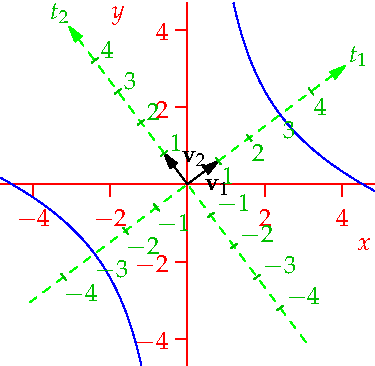
\includegraphics[scale=0.9]{quad-hyperbola}
\end{minipage}\smallbreak
\vspace{-10pt}
	\[Q_\beta^\epsilon =\frac 15\begin{pmatrix}
	4&-3\\3&4
	\end{pmatrix}\implies \twovec{t_1}{t_2}=[\vx]_\beta=Q_\epsilon^\beta\twovec xy=
	\frac 15\twovec{4x+3y}{-3x+4y}\]
	which quickly recovers the original conic by substitution.


\begin{minipage}[t]{0.64\linewidth}\vspace{0pt}
\item The conic defined by $K(\vx)=x^2+12xy+3y^2=-33$ defines a hyperbola in accordance with Example \ref{ex:diagbilinear}. With respect to the basis $\gamma=\{\stwovec 1{-2},\stwovec 01\}$, we see that
\begin{gather*}
K(\vx)=-11x^2+3(2x+y)^2=-11t_1^2+3t_2^2=-33\\
\iff \frac{t_1^2}{3}-\frac{t_2^2}{11}=1
\end{gather*}
Even though $\gamma$ is non-orthogonal, we can still plot the conic! If we instead used the orthonormal basis $\eta$, we'd obtain
\[K(\vx)=(\sqrt{37}+2)s_1^2-(\sqrt{37}-2)s_2^2=-33\]
however the calculation to find $\eta$ is time-consuming and the expressions for $s_1,s_2$ are extremely ugly.
\end{minipage}\begin{minipage}[t]{0.36\linewidth}\vspace{0pt}
\flushright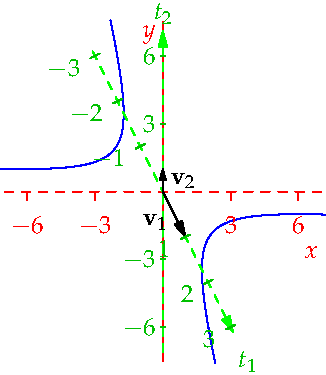
\includegraphics[scale=0.97]{quad-hyperbola2}
\end{minipage}
\end{enumerate}
\end{examples}

A similar approach can be applied to higher degree quadratic equations/manifolds: e.g.\ ellipsoids, paraboloids and hyperboloids in $\R^3$.

\vfil
 
\begin{exercises}
\exstart Prove that the sum of any two bilinear forms is bilinear, and that any scalar multiple of a bilinear form is bilinear: thus the set of bilinear forms on $V$ is a vector space.\vspace{-5pt}
  
\begin{enumerate}\setcounter{enumi}{1}
  \item[](\emph{You can't use matrices here, since $V$ could be infinite-dimensional!}) 
  \item Compute the matrix of the bilinear form
  \[B(\vx,\vy)=x_1y_1-2x_1y_2+x_2y_1-x_3y_3\]
  on $\R^3$ with respect to the basis $\beta=\left\{\sthreevec 101,\sthreevec 10{-1},\sthreevec 010\right\}$.
  
  \goodbreak
  
  \item Check that the function $B(f,g)=f'(0)g''(0)$ is a bilinear form on the vector space of twice-differentiable functions. Find the matrix of $B$ with respect to $\beta=\{\cos t,\sin t,\cos 2t,\sin 2t\}$ when restricted to the subspace $\Span\beta$.
  
  \item For each matrix $A$, find a diagonal matrix $D$ and an invertible matrix $Q$ such that $Q^TAQ=D$.
  \begin{enumerate}
    \item $\begin{pmatrix}
    1&3\\3&2
    \end{pmatrix}$\qquad
    (b)\ \ $\begin{pmatrix}
    3&1&2\\1&4&0\\2&0&-1
    \end{pmatrix}$
  \end{enumerate}
  
  \item If $K$ is a quadratic form and $K(\vx)=2$, what is the value of $K(3\vx)$?
  
  \item If $\F$ does not have characteristic 2, and $K(\vx)=B(\vx,\vx)$ is a quadratic form, prove that we can recover the bilinear form $B$ via
		\[B(\vx,\vy)=\frac 12\left(K(\vx+\vy)-K(\vx)-K(\vy)\right)\]
  
  \item If $B(\vx,\vy)=\vx^T\begin{smatrix}0&1\\1&0\end{smatrix}\vy$ is a bilinear form on $\F^2$, compute the quadratic form $K(\vx)$.
  
  \item Suppose $B$ is a symmetric bilinear form on a real finite-dimensional space. With reference to the proof of Sylvester's Law, explain why $\Rank B$ is independent of the choice of diagonalizing basis.
  
  \item If $\operatorname{char}\F\neq 2$, apply the diagonalizing algorithm to the symmetric bilinear form $B=\vx^T\begin{smatrix}0&1\\1&0\end{smatrix}\vy$ on $\F^2$. What goes wrong if $\operatorname{char}\F=2$? 
  
  \item Describe and plot the following conics:
  \begin{enumerate}
    \item $x^2+y^2+xy=6$
    
    \item $35x^2+120xy=4x+3y$
  \end{enumerate}
  
  \item Suppose that a non-empty, non-degenerate\footnotemark conic $C$ in $\R^2$ has the form $ax^2+2bxy+cy^2+dx+ey+f=0$, where at least one of $a,b,c\neq 0$, and define $\Delta=b^2-ac$. Prove that:
  \begin{itemize}
    \item $C$ is a parabola if and only if $\Delta=0$;
    \item $C$ is an ellipse if and only if $\Delta<0$;
    \item $C$ is a hyperbola if and only if $\Delta>0$.
  \end{itemize}
  (\emph{Hint: $\lambda_1,\lambda_2$ are the eigenvalues of a symmetric matrix, so\ldots})
  
  %\item Consider the quadratic form $K(x,y,z)=x^2+y^2-z^2$ which describes a cone in three dimensions. Let $ax+by+cz=1$ be the equation of a plane in $\R^3$ which does not pass through the origin. Prove that 
\end{enumerate}
\end{exercises}

\footnotetext{The conic contains at least two points and cannot be factorized as a product of two straight lines: for example, the following are disallowed;
  \begin{itemize}
    \item $x^2+y^2+1=0$ is empty (unless one allows conics over $\C\ldots$)
    \item $x^2+y^2=0$ contains only one point;
    \item $x^2-xy-x+y=(x-1)(x-y)=0$ is the product of two lines.
  \end{itemize}}
\clearpage

\iffalse

\setcounter{subsection}{10}
\subsection{The Geometry of Orthogonal Operators}

The purpose of this section is to classify the orthogonal operators $T\in\cL(V)$ on any finite-dimensional \emph{real} inner product space $V$. This is very easy to do when $\dim V=1$ or 2.

\begin{description}
	\item[\normalfont\emph{Dimension 1}:] Clearly $T(\vx)=a\vx$ for some $a\in\R$. $T$ is clearly self-adjoint and therefore orthogonal if and only if $a^2=1$, yielding $T=\pm I$.
	\item[\normalfont\emph{Dimension 2}:] Any choice of orthonormal basis $\beta$ generates an isomorphism of inner product spaces $\phi:V\to\R^2$ and the problem becomes that of identifying every orthogonal matrix in $M_2(\F)$. We already did this in Exercise \ref{ex:rotrefmatrix}: all orthogonal $2\times 2$ real matrices have the form
\[A_\theta=\begin{pmatrix}
	\cos\theta&-\sin\theta\\
	\sin\theta&\cos\theta
  \end{pmatrix},\qquad B_\theta=\begin{pmatrix}
	\cos\theta&\sin\theta\\
	\sin\theta&-\cos\theta
	\end{pmatrix}\]
for some $\theta\in\R$. Moreover, their effects are as follows:
	\begin{itemize}
	  \item $L_{A_\theta}\in\cL(\R^2)$ rotates vectors counter-clockwise about the origin by $\theta$ radians;
	  \item $L_{B_\theta}\in\cL(\R^2)$ reflects vectors across the line making angle $\frac 12\theta$ with the positive $x$-axis.
	\end{itemize}
\end{description}
	
These maps provides the motivation for a general definition of rotation and reflection.
	
\begin{defn}{}{}
Suppose $T\in\cL(V)$ where $V$ is a finite-dimensional real inner product space. We say that $T$ is a:
\begin{description}
  \item[\normalfont\emph{Rotation}] if either $T$ is the identity map, or if there exists a two-dimensional subspace $W\le V$ with orthonormal basis $\beta=\{\vx,\vy\}$ and some $\theta\in(0,2\pi)$ such that\footnote{We could include the identity here with $\theta=0$, but then \emph{any} 2-dimensional subspace $W$ is suitable and the axis of rotation is not well-defined.}
  \[T(\vx)=\cos\theta\,\vx+\sin\theta\,\vy,\qquad T(\vy)=-\sin\theta\,\vx+\cos\theta\,\vy,\qquad T(\vw^\perp)=\vw^\perp,\]
  for all $\vw^\perp\in W^\perp$, termed the \emph{axis of rotation.} Otherwise said, $[\at T{W}]_\beta=A_\theta$ and $\at T{W^\perp}=I$. 
  
  \item[\normalfont\emph{Reflection}] if there exists a one-dimensional subspace $W\le V$ such that $\forall \vw\in W,\vw^\perp\in W^\perp$,
  \[T(\vw+\vw^\perp)=-\vw+\vw^\perp\]
  Otherwise said, $\at T{W}=-I$ and $\at T{W^\perp}=I$. We could call this \emph{reflection across $W^\perp$.}
\end{description}
\end{defn}

\begin{example}{}{}
We compute the matrix of the reflection across $W^\perp=\Span\{\vi+2\vj\}\le\R^2$.\\[5pt]
First observe that $W=\Span\{2\vi-\vj\}$, whence $\beta=\{\stwovec 2{-1},\stwovec 12\}$ is an orthogonal basis (it doesn't need to be orthonormal!). The change of co-ordinate matrix from $\beta$ to the standard basis $\epsilon=\{\vi,\vj\}$ is $Q=Q_\beta^\epsilon=\begin{smatrix}
2&1\\-1&2
\end{smatrix}$, whence the required matrix is
\[A=Q_\beta^\epsilon\begin{pmatrix}
-1&0\\0&1
\end{pmatrix}Q_\epsilon^\beta =\frac 15\begin{pmatrix}
-3&4\\4&3
\end{pmatrix}\]
which is easily checked to satisfy $A\stwovec 2{-1}=-\stwovec 2{-1}$ and $A\stwovec 12=\stwovec 12$.
\end{example}

It should be clear that every rotation and reflection is an orthogonal operator and that they may be easily distinguished by determinant:
\[\det(\text{rotation})=1,\qquad \det(\text{reflection})=-1\]
It is also easy to see that $L_{A_\theta}\in\cL(\R^2)$ is a rotation as per the definition: simply take $\beta=\{\vi,\vj\}$ and $W=\R^2$! We leave the verification that $L_{B_\theta}\in\cL(\R^2)$ is a reflection as an exercise. The case for $\dim V=1$ is even easier. To summarize:

\begin{lemm}{}{22orth}
Suppose $V$ is a real inner product space with $\dim V=1$ or $2$. Then every orthogonal operator $T\in\cL(V)$ is either a rotation or a reflection.
\end{lemm}


Our goal is to describe any orthogonal operator $T$ in terms of rotations and reflections. The upshot is that there exists an orthonormal basis $\beta$ with respect to which the matrix of $T$ has block form
\[[T]_\beta=\diag(R_1,R_2,\ldots,R_k)\]
and each $R_j$ is either a $2\times 2$ rotation matrix, or is $\pm 1$.

\begin{example}{}{}
The matrix $A=\begin{smatrix}
\frac 35&-\frac 45&0&0\\
\frac 45&\frac 35&0&0\\
0&0&1&0\\
0&0&0&-1
\end{smatrix}$ describes an orthogonal operator $L_A\in\cL(\R^4)$. We have three commuting orthogonal operations $L_A=T_1T_2T_3$:
\begin{itemize}
  \item $T_1$ rotates by $\theta=\tan^{-1}\frac 43$ about the axis $W_1^\perp=\Span\{\ve_3,\ve_4\}$;
  \item $T_2$ is the identity rotation with `axis' $W_2^\perp=\Span\{\ve_1,\ve_2,\ve_4\}$;
  \item $T_3$ is reflection across $W_3^\perp=\Span\{\ve_1,\ve_2,\ve_3\}$
\end{itemize}
\end{example}

To see that this always happens, we first need a little theory regarding a real $n\times n$ matrix $A$. Our primary strategy relies on eigendecompositions; unfortunately $A$ need not have any \emph{real} eigenvectors. As a linear operator on $\C^n$ however, it must have at least one eigenpair $(\lambda,\vv)$: consider the real and imaginary parts: $\vv=\vx+i\vy$ and $\lambda=p+iq$ and observe that
\[A\vx+iA\vy=A(\vx+i\vy)=(p+iq)(\vx+i\vy)=(p\vx-q\vy)+i(p\vy+q\vx) \tag{$\ast$}\]
Since $A$ is real, we can equate real and imaginary parts to see that $\Span\{\vx,\vy\}$ \emph{is an $L_A$-invariant subspace of $\R^n$.} This is the generic situation, since, upon choosing a basis, any linear operator on a finite-dimensional real vector space is multiplication by some real matrix $A$. We therefore conclude:

\begin{lemm}{}{}
If $T\in\cL(V)$ is a linear operator on a finite-dimensional real vector space, then there exists a $T$-invariant subspace $W\le V$ such that $\dim W=1$ or 2.
\end{lemm}

The reason our construction might product a 1-dimensional space? The real and imaginary parts $\vx,\vy$ might be parallel! In this case, of course, $W$ is an eigenspace of $T$.\\

Of particular interest to our current goal is that the real and imaginary parts of ($\ast$) look very like a \emph{rotation.} Indeed if we specialize the Lemma to an orthogonal operator $T$, it is an easy exercise to check that $W^\perp$ is also $T$-invariant. We conclude that $\at T{W^\perp}$ is an orthogonal operator on a lower-dimensional vector space. We may now repeat the process until we have exhausted $V$. This leads to the following:

\begin{thm}{}{}
Let $T\in\cL(V)$ be an orthogonal operator on a finite-dimensional real inner product space. Then:
\begin{enumerate}
  \item There exists an orthogonal decomposition
	\[V= W_1\oplus\cdots \oplus W_m\]
	where each $W_k$ is a 1 or 2-dimensional $T$-invariant subspace.\footnote{It should be clear that $\frac n2\le m\le n$.}
	\item For each $j$, define $T_j:=\at T{W_j}+\at I{W_j^\perp}$. Then $T_j$ is a rotation or a reflection and $T=T_1\cdots T_m$.
	\item $\det T=(-1)^k$ where exactly $k$ of the $T_j$ are reflections.
	\item The subspaces may be chosen so that there is at most one reflection $T_j$, and where $\dim W_j=1$.
\end{enumerate}
\end{thm}

\begin{proof}
\begin{enumerate}
  \item We've already done this, though it could be made more formal by induction.
  \item Since $\at T{W_j}$ is orthogonal on a 1 or 2-dimensional space, Lemma \ref{lemm:22orth} says it is either a rotation or a reflection. Extending to $T_j$ by forcing the identity on $W_j^\perp$ produces a rotation or reflection on $\R^n$. Moreover, since the $W_j$ are orthogonal subspaces, we see that
  \[\vv_j\in W_j\implies T_k(\vv_j)=\begin{cases}
  T(\vv_j)&\text{if $j=k$}\\
  \vv_j&\text{if $j\neq k$}
  \end{cases}\]
  By applying to a basis where each $\vv_j$ lies in some $W_j$, the relationship $T=T_1\cdots T_m$ is now clear.
  \item This is immediate since every rotation has determinant 1 and every reflection determinant $-1$.
  \item Suppose that $T_j$ is a reflection and $\dim W_j=2$. Then there exists a one-dimensional subspace $\hat W_j$ such that
  \[\at{{T_j}}{{\hat W_j}}=-I,\qquad \at{{T_j}}{{\hat W_j^\perp}}=I\]
  By replacing $W_j$ by $\hat W_j\oplus \hat W_j^\perp$, we see that every reflection may be assumed to be one-dimensional.\\
  Now suppose $W_j,W_k$ are 1-dimensional subspaces corresponding to reflections $T_j,T_k$. Then
  \[(T_j+T_k)(\vv)=\begin{cases}
  -\vv&\text{if $\vv\in W_j\oplus W_k$}\\
  \vv&\text{if $\vv\in (W_j\oplus W_k)^\perp$}
  \end{cases}\]
  Otherwise said, $T_j+T_k$ is the \emph{rotation} with $W=W_j\oplus W_k$ and $\theta=\pi$. We can therefore replace an even number of reflections with rotations.\qedhere
\end{enumerate}
\end{proof}



% 
% \begin{lemm}{}{orthrotref}
% Every rotation is an orthogonal operator with determinant 1.\\
% Every reflection is an orthogonal operator with determinant $-1$.
% \end{lemm}\pagebreak[3]
% 
% \begin{proof}
% Given a rotation $T\in\cL(V)$ with axis $W^\perp$, extend the basis $\beta=\{\vx,\vy\}$ of $W$ to an orthonormal basis $\gamma$ of $V$. With respect to this basis, the matrix of $T$ has block form
% \[[T]_\gamma=\left(\begin{array}{c|c}
% A_\theta&0\\\hline
% 0&I
% \end{array}\right) \implies [T^*]_\gamma=\left(\begin{array}{c|c}
% A_\theta^T&0\\\hline
% 0&I
% \end{array}\right)
% =\left(\begin{array}{c|c}
% A_\theta^{-1}&0\\\hline
% 0&I
% \end{array}\right) =[T]_\gamma^{-1}\]
% since $A_\theta$ is orthogonal. We conclude that $T$ is invertible with inverse $T^{-1}=T^*$: that is, $T$ is an orthogonal operator. Moreover its determinant is clearly $\det A_\theta=1$.\\[5pt]
% We leave the reflection argument as an exercise.
% \end{proof}



\begin{example}{}{orthorotatenasty}
Consider the matrix $A=\frac 1{25}\begin{smatrix}
  15&-12&-16\\
  20&9&12\\
  0&-20&15
  \end{smatrix}$. We show that $L_A\in\cL(\R^3)$ is a rotation and find its axis and angle of rotation.\\[5pt]
  It is easy (with a calculator!) to check that $A^TA=I$ so that $A$ is orthogonal, and moreover that $\det A=1$.
  %\[\det A=\frac 1{25^3}\left(15^2\cdot 9+16\cdot 20^2+2\cdot 12\cdot 15\cdot 20\right)=1\]
  According to the Theorem, there are no reflections in $A$ and so there must exist a decomposition $\R^3=W\oplus W^\perp$ where $\dim W=2$ and such that $W^\perp$ is an eigenspace with eigenvalue 1. We can hunt for the eigenvalues via the usual approach, or we can do it by brute force: $\vw^\perp=\sthreevec abc$ has eigenvalue 1 if and only if
   \[\begin{cases}
   15a-12b-16c=25a\\
   20a+9b+12c=25b\\
   -20b+15c=25c
   \end{cases} \iff c=-2b, \ a=2b \iff \vw^\perp\propto\threevec 21{-2}\]
   The axis of rotation is therefore $W^\perp=\Span\left\{\sthreevec 21{-2}\right\}$. To find the angle, we simply need to choose anything orthogonal to this (and therefore in $W$), and see how $A$ changes the angle. Thus let $\vw=\sthreevec 101$ and compute
   \[A\vw=\frac 1{25}\threevec{-1}{32}{15}\implies \cos\theta=\frac{\sthreevec 101\cdot\sthreevec{-1}{32}{15}}{ \sqrt{1+1}\sqrt{1+32^2+15^2}}
   =\frac{14}{50}=\frac 7{25} \implies \theta\approx \ang{74}\]
   In fact $(\vw,A\vw,\vw^\perp)$ is negatively oriented if we `look down' on $W=\Span\{\vw,A\vw\}$ from above $\vw^\perp$, the rotation would be through  \ang{74} \emph{clockwise.}
\end{example}

Because of the theorem, some authors prefer to simply define a rotation to be any orthogonal operator with determinant 1 and a reflection to be any with determinant $-1$. The multiplicative property of determinant then shows that the composition of any two rotations is a rotation,\footnote{In particular, this shows that the set of `rotations' forms a normal subgroup $\rSO(V)$ of the group of orthogonal operators on $V$, known as the \emph{special orthogonal group.}} of two reflections is a rotation, etc. The problem with this definition is that one loses the notion of an axis of rotation, since a general determinant 1 orthogonal operator will typically require multiple rotations around several axes.

\begin{example}{}{}
For given $\theta,\phi$, the matrix
\[A=\begin{smatrix}
  \cos\theta&-\sin\theta&0&0\\
  \sin\theta&\cos\theta&0&0\\
  0&0&\cos\phi&-\sin\phi\\
  0&0&\sin\phi&\cos\phi
\end{smatrix}\]
performs two rotations. It has no `axis' of rotation, since it has no eigenspace with eigenvalue 1: indeed it has no \emph{real} eigenvalues at all. Regardless, it is orthogonal and has determinant 1, so many authors consider this to be a rotation.
\end{example}

\begin{exercises}
\exstart Find the matrices with respect to the standard basis of the reflections in $W^\perp$:

\begin{enumerate}
	\item[]\begin{enumerate}
	  \item $W=\Span\{-2\vi+5\vj\}$
	  \item $W=\Span\{\vi+2\vj+2\vk\}$\quad  \emph{Hint: consider the basis $\beta=\left\{\frac 13\sthreevec 122,\frac 13\sthreevec 2{-2}1,\frac 13\sthreevec 21{-2}\right\}$}
	\end{enumerate}
	
  \item\begin{enumerate}
  	\item Given $\phi$, let $\beta=\{\vx,\vy\}=\left\{\stwovec{\cos\phi}{\sin\phi},\stwovec{-\sin\phi}{\cos\phi}\right\}$ and $\gamma=\{\vx,-\vy\}$. Clearly every orthonormal basis of $\R^2$ has the form $\beta$ or $\gamma$. Compute the matrices
  	\[[L_{A_\theta}]_\beta\quad\text{and}\quad[L_{A_\theta}]_\gamma\quad\text{where}\quad A_\theta=\begin{pmatrix}
		\cos\theta&-\sin\theta\\
		\sin\theta&\cos\theta
  	\end{pmatrix}\]
  	What do you observe?
  	\item Now consider the reflection matrix $B_\theta=\begin{smatrix}
		\cos\theta&\sin\theta\\
		\sin\theta&-\cos\theta
  	\end{smatrix}$. Show that there is a privileged orthonormal basis (indeed four up to scaling and reordering) $\beta$ such that $[L_{B_\theta}]_\beta=\begin{smatrix}
		1&0\\
		0&-1
  	\end{smatrix}$.
 	\end{enumerate}
 	
 	\item Compute $A_\phi B_\theta A_\phi^{-1}$. Across what line in $\R^2$ does this matrix reflect? Can you do this \emph{without} multiplying out the matrices?
  
  \item Prove explicitly:
  \begin{enumerate}
    \item If $T$ is a rotation then it is orthogonal and $\det T=1$;
    \item If $T$ is a reflection then it is orthogonal and $\det T=-1$.
  \end{enumerate}
  
  \item If $W$ is a $T$-invariant subspace where $T$ is an orthogonal operator on a finite-dimensional real inner product space $V$, prove that $W^\perp$ is also $T$-invariant.

	\item Find the result when the vector $\vx=\sthreevec 342$ is rotated \ang{90} counter-clockwise around the $z$-axis (when viewed from above) and then reflected in the $xz$-plane. What is the effect of this transformation on a general vector?
  
  \item For any non-zero $\theta,\phi\in(-\pi,\pi)$, define the matrices
  \[A=\begin{pmatrix}
  \cos\theta&-\sin\theta&0\\
  \sin\theta&\cos\theta&0\\
  0&0&1
  \end{pmatrix}\qquad B=\begin{pmatrix}
  1&0&0\\
  0&\cos\phi&-\sin\phi\\
  0&\sin\phi&\cos\phi
  \end{pmatrix}\]
  Prove that $L_{AB}$ is a rotation of $\R^3$ and find its axis of rotation.

 	
%  	 since it has eigenspaces
% \[W=E_{-1}=\Span\left\{\twovec{-\sin\frac\theta 2}{\cos\frac\theta 2}\right\},\qquad W^\perp=E_1=\Span\left\{\twovec{\cos\frac\theta 2}{\sin\frac\theta 2}\right\}\]
  
%  
%   
%   \item Recall (Exercise \ref{ex:unitarymatrix}) that a unitary matrix $A\in M_n(\C)$ has an orthonormal eigenbasis $\gamma=\{\vect{\vv}{n}\}$ and eigenvalues $e^{i\theta_1},\ldots,e^{i\theta_n}$.
%   \begin{enumerate}
%     \item Suppose $A$ is real (it is an \emph{orthogonal} matrix). Prove that each $\cl{\vv_j}$ is also an eigenvector with eigenvalue $e^{-i\theta_j}$.
%     \item If $e^{i\theta_j}$ is not real, show that $\dim\Span\{\vv_j,\cl{\vv_j}\}=2$. Moreover, find a 2-dimensional subspace $W$ of $\R^n$ so that $L_A$ restricted to $W$ is a rotation by angle $\theta_j$.
%     \item If $e^{i\theta_j}$ is real, show that there exists a 1 or 2-dimensional subspace $W$ of $\R^n$ such that $L_A$ restricted to $W$ is $\pm I$.
% 	\end{enumerate}
	
	\item Let $V$ be a real inner product space of dimension 2. Given any $\vx\neq \vy$ with $\Nm\vx=\Nm\vy=1$, show that there exists a unique rotation $T\in\cL(V)$ such that $T(\vx)=\vy$.
% 	  \item (If you've done group actions in group theory) Write $\rSO(n+1)$ for the special orthogonal group $\rSO(\R^{n+1})$. Part (a) shows that the action of the group $\rSO(n+1)$ is transitive on $S^n$. Given $\vx\in S^n$ consider the \emph{stabilizer} subgroup
% 	  \[\Stab(\vx)=\{U\in\rSO(n+1):U(\vx)=\vx\}\]
% 	  Prove that $\Stab(\vx)\cong\rSO(n)$ and moreover that there exists a bijection of the unit sphere with the set of left cosets
% 	  \[\mu:S^n\to\quotient{\rSO(n+1)}{\rSO(n)}=\{TU:T\in\rSO(n+1),U\in\Stab(\vx)\}\]
% 	  (\emph{This `transitive action modulo stabilizer' construction is known as a homogeneous space})
% 	\end{enumerate}
\end{enumerate}
\end{exercises}

\fi


\fi